\documentclass[10pt,twoside,a4paper,fleqn]{report}
\usepackage{etex} % required for tikz figures
\usepackage[english,st]{rpg} % select type {semester}/bachelor/master thesis: {st}/bt/mt
\usepackage{amsmath}
\usepackage{amssymb}
\usepackage{cancel}
\usepackage{IEEEtrantools}
\usepackage[font=small,labelfont=bf]{caption}
\usepackage{amsfonts}
\usepackage{multirow}

% Page header (don't change)____________________________________________________
\setlength{\parindent}{0em}                 % Disable parindent
\rhead[\nouppercase{\rightmark}]{\thepage}  % Special headings
\lhead[\thepage]{\nouppercase{\leftmark}}   % Special headings
\cfoot{}                                    % Special headings

%%%%%%%% Hint %%%%%%%%%%%
% Define your custom stuff here, e.g. Symbols that you are using. If you define them here it is easy to change them later on if you run into a nomenclature conflict.
\newcommand{\mysymbol}[0]{\mathbf{S}_{my}}   % custom symbol which can easily be changed if necessary
\newcommand{\bomega}[0]{\boldsymbol{\omega}} % bold greek letter
\newcommand{\bSymb}[1]{\mathbf{#1}}			% toy example with one argument

% tikz plots
\pgfplotsset{compat=newest}
\pgfplotsset{plot coordinates/math parser=false}
\pgfplotsset{yticklabel style={text width=2em,align=right}}
\newlength\fheight
\newlength\fwidth

% Figures from Inkscape
\graphicspath{{img//}}

% Title page (please fill in)___________________________________________________
\title{Improving Inertial Odometry using Machine Learning}

\studentA{Guillem Torrente-Marti}
\ethidA{46-947-606}
\emailA{tguillem@student.ethz.ch}

% \studentB{Second Student}
% \ethidB{12-345-678}
% \semesterB{9}
% \emailB{second@student.ethz.ch}

\supervision{Zichao Zhang\\ Elia Kaufmann\\ Prof. Dr. Davide Scaramuzza}
\date{May 2019}

\infopage
\declaration

% Begin document________________________________________________________________
\begin{document}
\maketitle 							      % Create title page

% Preamble______________________________________________________________________
\pagenumbering{roman} 				% Begin roman page numbering (i,ii,...)
%---------------------------------------------------------------------------
% Table of contents

 \setcounter{tocdepth}{2}
 \tableofcontents
 \cleardoublepage

%---------------------------------------------------------------------------
% List of Figures

 \addcontentsline{toc}{chapter}{List of Figures}
 \listoffigures
 \clearpage

%---------------------------------------------------------------------------
% List of Tables

 % \addcontentsline{toc}{chapter}{List of Algorithms}
 % \listofalgorithms
 % \clearpage

%---------------------------------------------------------------------------
% Abstract

\chapter*{Abstract}
\addcontentsline{toc}{chapter}{Abstract}

Almost any mobile robot nowadays is equipped with an Inertial Measurement Unit, an electronic sensor which provides high-rate observations of its acceleration and angular velocity states. 
Unfortunately, these sensors are usually very noisy, and unless paired with some other complementary source of state estimation, have shown to be unreliable for 3D Inertial Odometry (IO).
In this report, we investigate how supervised deep learning can help to make the problem more feasible.
We review the existing ideas in the state-of-the-art, and implement several artificial neural architectures for increasingly demanding tasks. 
By iteratively building on the results, we finally address the task of 3-fold state integration for position, velocity and orientation states.
We propose three different formulations of the learning problem that all demonstrate to be effective at reducing the effect of IMU drift, which shows the first progresses towards a more reliable deep IO pipeline. 
Although still not fully developed, the last of these three studied approaches is an original formulation derived from the mapping of the rotation state to its Lie Algebra space, and the usage of an IMU pre-integration theory recently proposed.
We finally propose several interesting ways to continue fine-tuning our current state estimator towards a more context-aware probabilistic model.
    
\cleardoublepage

%---------------------------------------------------------------------------
% Symbols

\chapter*{Nomenclature}\label{chap:symbole}
\addcontentsline{toc}{chapter}{Nomenclature}

\section*{Notation}
  \begin{tabbing}
    \hspace*{1.6cm}   \= \kill
    $\mathbf{J}$       \> Jacobian \\[0.5ex]
    $\mathbf{T}_{WB}$  \> coordinate transformation from frame $B$ to frame $W$ \\[0.5ex]
    $\mathbf{R}_{WB}$  \> orientation of $B$ with respect to $W$ \\[0.5ex]
    $_W\mathbf{t}_{WB}$\> translation of $B$ with respect to $W$, expressed in coordinate system $W$ \\[0.5ex]
  \end{tabbing}
  
Scalars are written in lower case letters ($a$), vectors in lower case bold letters ($\mathbf{a}$) and matrices in upper case bold letters ($\mathbf{A}$).

\section*{Acronyms and Abbreviations}
  \begin{tabbing}
    \hspace*{1.8cm}  \= \kill
    DoF     \> Degree of Freedom \\[0.5ex]
    IMU     \> Inertial Measurement Unit \\[0.5ex]
    MAV     \> Micro Aerial Vehicle \\[0.5ex]
    ROS     \> Robot Operating System \\[0.5ex]
    MEMS    \> Micro-Electro-Mechanical systems \\[0.5ex]
    (V)IO   \> (Visual-)Inertial Odometry  \\[0.5ex]
    ML      \> Machine Learning  \\[0.5ex]
    DL      \> Deep learning  \\[0.5ex]
    NN      \> Neural Network  \\[0.5ex]
    CNN     \> Convolutional Neural Network  \\[0.5ex]
    RNN     \> Recurrent Neural Network  \\[0.5ex]
    LSTM    \> Long Short-Term Memory \\[0.5ex]
    GRU     \> Gated Recurrent Unit \\[0.5ex]
    (E)KF   \> (Extended) Kalman Filter \\[0.5ex]
    (R)MSE  \> (Root) Mean Squared Error  \\[0.5ex]
    BB      \> BlackBird (dataset)  \\[0.5ex]
    STFT    \> Short-Time Fourier Transform  \\[0.5ex]
    SO(3)   \> Special Orthonormal group \\[0.5ex]
    SE(3)   \> Special Euclidean group \\[0.5ex]
    
  \end{tabbing}

\clearpage

%---------------------------------------------------------------------------


% Chapters______________________________________________________________________
\pagestyle{fancy}             % Fancy headings
\pagenumbering{arabic}				% Begin arabic page numbering (1,2,...)

\chapter{Introduction}\label{chap:introduction}

Inertial Sensor Units (IMU's) have become an everyday sensor in all kinds of devices, ranging from smart phones, drones, ships, autonomous cars or virtual reality headsets among others. 
One of the main reasons for that, is that they are conveniently complementary to the information that cameras capture, which are commonly found too in these devices. 
While the latter provide exteroceptive information about appearance and geometry up to scale, IMU's are proprioceptive sensors that make the previously unknown metric scale observable \cite{DBLP:journals/corr/ForsterCDS15}. 
Other reasons for their extended use are also their low power consumption, or the fact that they work even in darkness, or in GPS-denied environments \cite{DBLP:journals/corr/abs-1712-09004}.

However, either because of weight, space or economic constraints, most times the IMU's employed in these applications must be reduced in scale. 
Nowadays, \emph{Micro-electro-mechanical systems} (MEMS) have enabled to manufacture small and cheap enough IMU's, but these attributes come at the expense of higher sensor noise \cite{DBLP:journals/corr/abs-1802-02209}. 
Even if such noise is small, this renders traditional IMU integration unreliable as an Odometry method, as small errors in orientation lead to the so-called \emph{gravity leak} problem.
This phenomenon acts as a positive-feedback source of noise in position estimation, which in its turn results in a rapidly increasing drift of the estimation from the correct value \cite{Woodman07anintroduction}. 

Currently, there's a large variety of techniques that aim at leveraging other data input sources like cameras, or constraints/priors as for instance planar 2D motion, to cope with the IMU drift. 
Even so, the problem of Odometry in agile aerial robots (a 3D problem setup) remains a largely unsolved problem, and especially in the case of standalone Inertial Odometry (IO) \cite{DuoVIO}. 

On the other hand, Machine Learning (ML) and in particular Deep Learning (DL), have undergone a significant expansion in the last 10 years since the publication of AlexNet in 2012. 
In fact, recent approaches at odometry pipelines already include DL models to help solve this problem \cite{DBLP:journals/corr/abs-1802-02209, DBLP:journals/corr/ClarkWWMT17, DBLP:journals/corr/abs-1803-05850}.

In this thesis, we aim at progressing the research of Inertial navigation using a DL strategy. 
We will be combining ideas from several state-of-the-art publications into three IO-related state estimation pipelines, and analyzing their results. 
Because of that, in this work we will step away from any leveraging technique that uses inertial measurements combined with any other source of state observations, and tackle the problem of IO right at its core.
Furthermore, we will be using 3D datasets recorded by aerial units, as this is the most challenging form of the problem we can encounter with aboundant training data, where for instance assumptions on planar motion are not valid.


\section{Related Work}\label{sec:related_work}

In this section we will be reviewing several recent publications that have proposed novel methods of working with inertial data with a deep learning setup. 
We will be paying special attention to the studies that tackle the specific problem of IO, but we will also be exploring other approaches of IMU processing using DL in a broader VIO pipeline.

\subsection{Convolutional Neural Networks for speed regression}\label{sec:speed_reg}
The first work that we want to discuss is a very recent effort by Cort\'es et.al.  \cite{DBLP:journals/corr/abs-1808-03485}, which in fact inspired this project. 
In their work, a Convolutional Neural Network (CNN) regressor is used to predict the speed (i.e. the average modulus of the velocity vector $\hat{s} = \left \| \mathbf{\hat{v}}\right \|$) over a window of time (see Figure \ref{fig:original_speed_net}) just from its IMU measurements. 
The datasets used in this study are recorded by several people with a smartphone, making different walking patterns.
Their objective is to use the calculated speed values provided by the CNN model in a nonlinear state estimation pipeline, to track the position of the user over time. 

\begin{figure}[h]
   \centering
   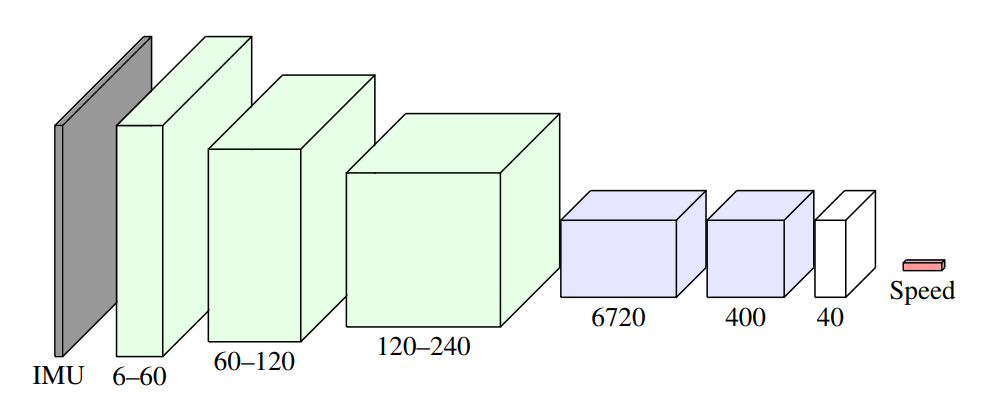
\includegraphics[width=0.75\textwidth]{thesis_template/img/cortes_cnn_architecture.png}
   \caption{CNN architecture from \cite{DBLP:journals/corr/abs-1808-03485}. This model is trained to estimate the speed norm of a moving object from a windowed sequence of IMU data. 
   Green layers are convolutional and the rest are fully connected (white does not have activation).}
   \label{fig:original_speed_net}
\end{figure}


In particular, the CNN model $f_\theta(\cdot)$ parametrized by $\theta$ estimates $\hat{s}$ using a $w\times6$ array of IMU data. 
Here \emph{w} is am hyper-parameter describing the number of IMU samples used as input, and 6 refers to the 6 Degree-of-Freedoms (DoF) of data captured by the IMU. 
In this case and during the rest of this report, IMU data will be assumed of 6 DoF (3 for gyroscope and 3 for accelerometer).
In other words, the model performs the computation described by \ref{eq:cnn_speed_regression}: 
\begin{equation}\label{eq:cnn_speed_regression}
    f_\theta\left(\mathbf{\hat{M}}_{k}\right) \rightarrow \hat{s}(k), \;\;\; \mathbf{\hat{M}}_{k}\in\mathbb{R}^{w\times6}, \;\hat{s}(k)=\left \| \mathbf{\hat{v}}(k)\right \|\in\mathbb{R}, \; \mathbf{\hat{v}}(k)\in\mathbb{R}^3.
\end{equation}
Where the variable \emph{k} refers to an arbitrary discrete time sample, such that $\mathbf{\hat{M}}_k$ comprises \emph{w} time samples between $\mathbf{\hat{M}}\!\left(k-w\right)$ and  $\mathbf{\hat{M}}\!\left(k\right)$. 
Indeed, $\mathbf{\hat{M}}$ includes both the information of the gyroscope and accelerometer, and has the structure given in \ref{eq:imu_img}.
\begin{equation}\label{eq:imu_img}
    \mathbf{\hat{M}}_k = \begin{bmatrix}
        _{B}\mathbf{\hat{a}}(k-w) & _{B}\mathbf{\hat{\boldsymbol{\omega}}}(k-w)\\ 
        _{B}\mathbf{\hat{a}}(k-w+1) & _{B}\mathbf{\hat{\boldsymbol{\omega}}}(k-w+1)\\ 
        \vdots & \vdots \\ 
        _{B}\mathbf{\hat{a}}(k) & _{B}\mathbf{\hat{\boldsymbol{\omega}}}(k)\\  
        \end{bmatrix} \in\mathbb{R}^{w\times6}.
\end{equation}
$\mathbf{\hat{M}}_k$ is composed by $_{B}\mathbf{\hat{a}}$ and $_{B}\mathbf{\hat{\boldsymbol{\omega}}}$, which are the observed acceleration and angular rates with the IMU respectively.
We will use the \emph{hat} ($\;\hat{}\;$) operator to indicate an estimated (or noisily observed) value, and \emph{k} and \emph{t} to refer to discrete and continuous time indices respectively from now on.
As a consequence, $\hat{s}(k)$ is the estimated \emph{average} speed during the time window between $(k-w, k)$. 
Such value predicted by the model is then fed as a low-confidence measurement update in an Extended Kalman Filter (EKF) pipeline \cite{DBLP:journals/corr/SolinCRK17}. 
For this particular study, the authors were using a 100Hz inertial sensor, and a two second window of data, i.e. $w = 200$.

The performance of their deep speed regressor is tested against a pedestrian dataset containing walking, static, stair climbing sequences, and achieves a RMSE error of $0.2\; m/s$.
Despite this, the performance of the model is worse than that for the stair sequences, which the authors justify as a lack of training samples of that particular type. 

\subsection{Recurrent Neural Networks for 2D IO}\label{sec:ionet}

This next work by Chen et.al. \cite{DBLP:journals/corr/abs-1802-02209} is somewhat more ambitious than the previous one, in the sense that it aims at performing end-to-end in-plane inertial odometry with, once again, walking datasets. 
In this planar setup, the agent state $\mathbf{x}$ can be defined by three degrees of freedom: two for position ($x$, $y$) and one for orientation/yaw ($\psi$). 
Similarly than before, the aim is to predict the state $\mathbf{x}(t+\Delta t)$ using only the IMU measurements belonging to the time window between $t$ and $t + \Delta t$.

However, as indicated by the authors of this paper, and interestingly unnoticed by the authors of \cite{DBLP:journals/corr/abs-1808-03485}, this problem setup is an ill-posed one.
This is because to predict the state $\mathbf{x}(t+\Delta t)$ the initial state $\mathbf{x}(t)$ is necessary, and therefore the IMU data alone is not enough for this task. 
Fortunately, the authors are able to demonstrate that by reformulating the problem into predicting the state increment $\Delta\mathbf{x} = (\Delta x, \Delta y, \Delta \psi)^{T}$, then the solution becomes independent of the initial state. 
In fact, it is possible to reduce the DoF of $\Delta\mathbf{x}$ further to only 2 by means of polar coordinates: $(\Delta l, \Delta \psi)^{T}$

In particular, as shown in \ref{eq:state_change_formulation}, the authors derive a formulation where the state increment $\Delta\mathbf{x}$ is a function of the initial velocity, gravity vector and IMU readings (all in body frame).
In theory, it is therefore possible to build a parametrized model $f_\theta$ such that it calculates the state shift from these inputs:
\begin{equation}\label{eq:state_change_formulation}
    f_\theta\left(_B\mathbf{g}(t), _{B}\mathbf{v}(t),_{B}\!\mathbf{\hat{a}}(t\!:\!t+\Delta t),_{B}\!\mathbf{\hat{\boldsymbol{\omega}}}(t\!:\!t+\Delta t)\right)\rightarrow\Delta\mathbf{x}, \;\;\;_{B}\mathbf{\hat{a}}, _{B}\!\mathbf{\hat{\boldsymbol{\omega}}}\in\mathbb{R}^3.
\end{equation}
Notice that the entire formulation works with 3D vectors, although the z position is assumed to be constant.
Furthermore, the authors argue that it is possible that the variables $\mathbf{g}(t)$ and $\mathbf{v}(t)$ are in fact latent variables of the sequence $\left(\mathbf{\hat{a}}(t\!:\!t+\Delta t),\mathbf{\hat{\boldsymbol{\omega}}}(t\!:\!t+\Delta t)\right)$, where the $B$ subindex has been dropped for readability. 

With this idea, the discrete time deep regressor would compute the estimated state increment as shown in \ref{eq:ionet_state_increment}.
\begin{equation}\label{eq:ionet_state_increment}
    f_\theta(\mathbf{\hat{M}}_{k}) \rightarrow \Delta\mathbf{\hat{x}}(k), \;\;\; \mathbf{\hat{M}}_{k}\in\mathbb{R}^{w\times6}, \;\Delta\mathbf{\hat{x}}(k)\in\mathbb{R}^{2}.
\end{equation}
Where again $\mathbf{\hat{M}}_{k}$ are the IMU measurements over a window of time equivalent to $\Delta t$. Finally, the estimated state increment $\Delta\mathbf{\hat{x}}=(\Delta \hat{l}, \Delta \hat{\psi})^{T}$, is used to compute $\mathbf{\hat{x}}(k+w)$ from $\mathbf{x}(k)$ as specified in \ref{eq:state_increment_2d}.
 \begin{equation}\label{eq:state_increment_2d}
     \mathbf{\hat{x}}(k+w)=\mathbf{x}(k) +
    \begin{bmatrix} 
    \Delta \hat{l}\cdot\cos\left(\psi(k)+\Delta\hat{\psi}\right) \\
    \Delta \hat{l}\cdot\sin\left(\psi(k)+\Delta\hat{\psi}\right) \\ 
    \Delta\hat{\psi} 
    \end{bmatrix}.
 \end{equation}

Another interesting point of this article is that, with the reasoning that IMU data has a strong temporal dependence over a window of time, Recurrent Neural Networks (RNN's) may be an interesting architecture to extract temporally correlated features out of it.
In particular, their expectation is that this kind of layer will be able to extract the missing latent variables $\mathbf{g}(t)$ and $\mathbf{v}(t)$ from the IMU measurements sequences, therefore rendering the problem completely independent of any variable except from $\mathbf{\hat{M}}_{k}$.
In particular, they use the Long Short-Term Memory (LSTM) architecture \cite{hochreiter1997long}, which has been shown to preserve better the gradients over time than its vanilla Recurrent layer counterpart \cite{DBLP:journals/corr/GreffSKSS15}. 

Their proposed deep model is actually quite simple, as it consists of simply two stacked LSTM layers (see Figure \ref{fig:original_ionet}). 
The first one creates a 96-dimensional hidden state (with ideally the latent variables), which serves as input to the second layer. 
The latter finally spits out a 2-dimensional value, corresponding to the polar state increment $\Delta\mathbf{\hat{x}}$. 
In fact, they empirically show that by using a \emph{bidirectional} LSTM layer (i.e. a layer that uses both past and future data to predict the displacement), the model gains slight benefits in training time compared to the non-bidirectional approach. 
Furthermore, they also train a CNN model for comparison purposes, which is shown to train considerably slower than the LSTM. 
Unfortunately, no further details about this CNN model architecture are provided.

\begin{figure}[h]
   \centering
   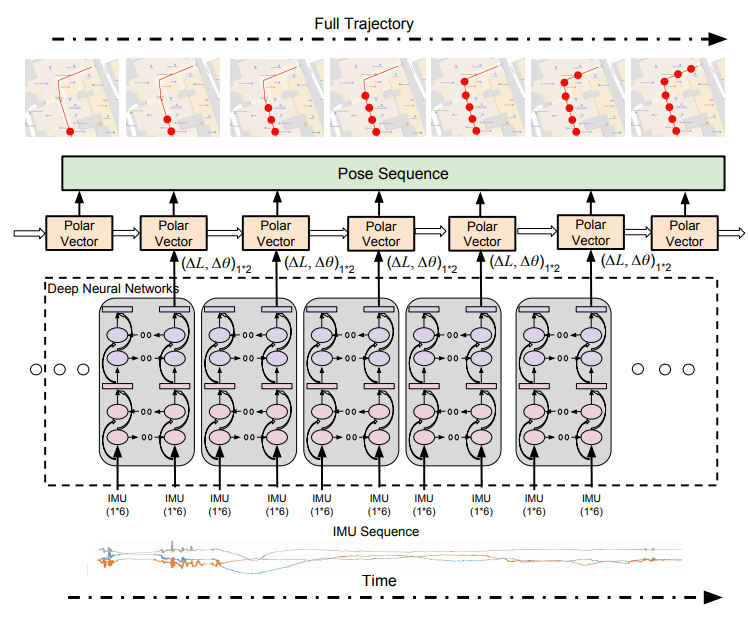
\includegraphics[width=0.75\textwidth]{thesis_template/img/ionet_original_architecture.png}
   \caption{RNN architecture from \cite{DBLP:journals/corr/abs-1802-02209} that predicts polar state increments in 2D (position + rotation) from IMU data. Two concatenated LSTM layers process the inertial input, and output a two component vector corresponding to the predicted the state increment $\Delta\mathbf{\hat{x}}$. This is later applied to the previous poses to generate a new pose in the sequence.}
   \label{fig:original_ionet}
\end{figure}
\subsection{Other usages of DL in Visual-Inertial Odometry}

The two previously introduced studies were thoroughly discussed as they both strictly fit in the use case of DL for IO (or closely related) purposes.  
However, there are other works that are worth mentioning in which DL is employed in the Visual-Inertial Odometry (VIO) problem. 

\subsubsection{Multirate CNN-RNN based VIO}\label{sec:VIOnet}
For instance, Clark and his team proposed in 2017 the idea of embedding a CNN network with an LSTM-based architecture in a VIO pipeline \cite{DBLP:journals/corr/ClarkWWMT17}. 
In particular, the convolutional layers are used to extract a low-rate feature vector from the optical flow between two image frames, and the recurrent ones to do the same at a higher rate with an IMU. 
Both outputs are then combined into a second (core) LSTM model that generates, similarly to \cite{DBLP:journals/corr/abs-1802-02209}, a state increment $\Delta\mathbf{\hat{x}}$.
Such increment prediction is then concatenated with the previous state estimate, and fed back to the core LSTM. The architecture schematic from the original publication is provided in Figure \ref{fig:original_vionet}. 

\begin{figure}[h]
   \centering
   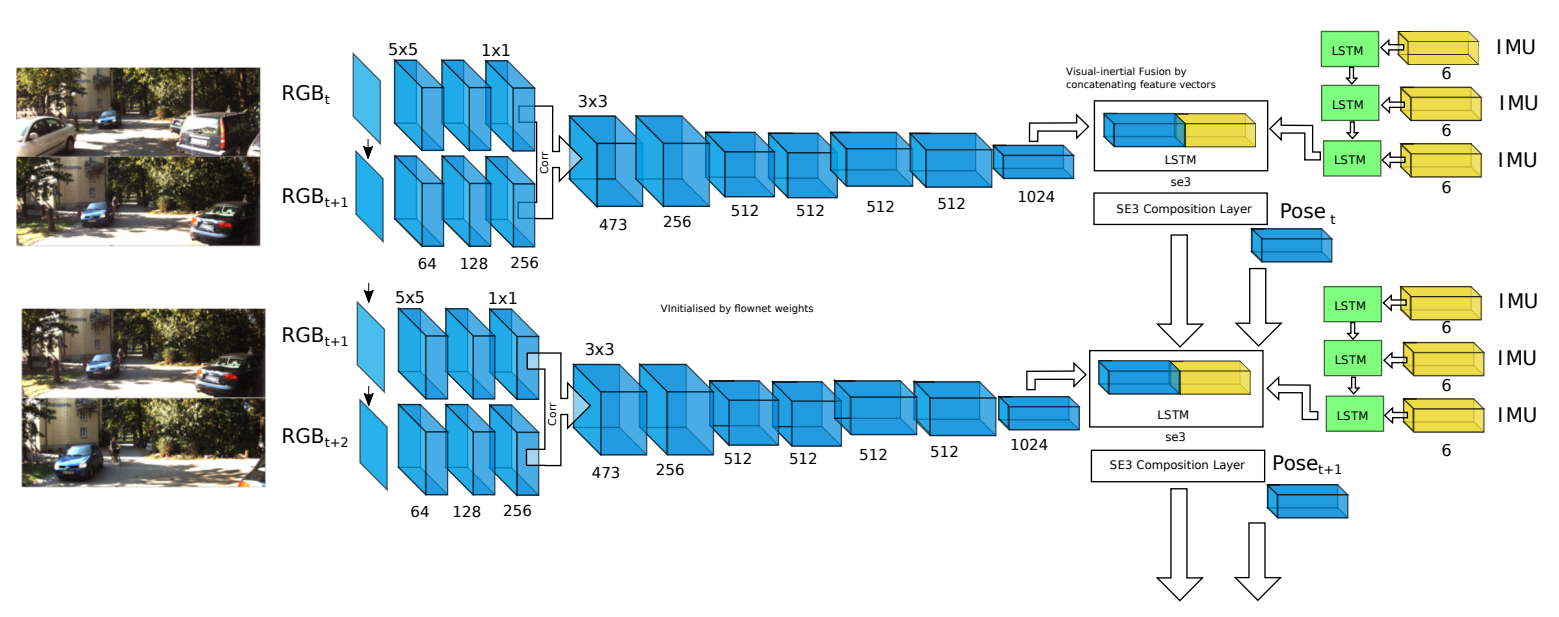
\includegraphics[width=0.90\textwidth]{thesis_template/img/vionet_original_architecture.png}
   \caption{CNN-RNN architecture from \cite{DBLP:journals/corr/ClarkWWMT17} for VIO. A CNN sequentially processes the image frames, while an LSTM processes the IMU data. Both feature vectors are concatenated and fed to a second LSTM, which predicts the state increment. Since the IMU rate is higher than the image rate, the core LSTM is adjusted to handle this rate difference.}
   \label{fig:original_vionet}
\end{figure}

Although it is unclear how reliant this model is to its Inertial part compared to the visual part, their proposed method achieves a performance close to the OK-VIS algorithm \cite{okvis} in the EuRoC \cite{Burri25012016} Micro-Aerial Vehicle (MAV) 3D dataset and in the outdoors autonomous driving KITTI dataset \cite{Geiger2012CVPR, Geiger2013IJRR}. 
Furthermore, it proves to be arguably more robust than OK-VIS in the situations where the extrinsic calibration between the IMU and the camera is not ideal. 

Last but not least, this paper is the first to our knowledge that introduces the idea of using the Lie algebra representation of the rotation group $SO(3)$ to help during the training of the deep model.
More insights about this will be discussed in Section \ref{sec:lie_algebra}.

\subsubsection{Unsupervised VIO with online error correction}
Another interesting although a bit more divergent approach is described by Shamwell et. al. in \cite{DBLP:journals/corr/abs-1803-05850}. 
This time, the VIO problem is faced from the unsupervised point of view, as they build a model that iteratively estimates and improves an affine transformation matrix that maps an input image at time $t$ to a target image at time $t+\Delta t$.
Indeed, it is assumed that some transformation has occurred during $\Delta t$, such that the images are slightly unaligned.
Note that with this strategy, no need for ground truth is needed.

Using the same notation as with the previous equations, the optimization starts by a CNN model $f_\theta(\cdot)$ extracting features from a window of IMU samples $\mathbf{\hat{M}}_k$ ranging from time $k-w$ until $k$. 
The same convolutional network also outputs the six degrees of freedom $\hat{\boldsymbol{\theta}}_0(k)\!\in\mathbb{R}^6$ of an affine transformation matrix, where the subindex $0$ indicates that this is the first iteration of the refinement).
\begin{equation}
    f_\theta\left(\mathbf{\hat{M}}_{k}\right) \rightarrow \hat{\boldsymbol{\theta}}_0(k), \;\;\; \mathbf{\hat{M}}_{k}\in\mathbb{R}^{w\times6}, \;\hat{\boldsymbol{\theta}}_0(k)\in\mathbb{R}^6
\end{equation}
Then, $\hat{\boldsymbol{\theta}}_0(k)$ is used to warp the input image $\mathbf{I}(k-w)$, producing an estimate image $\mathbf{\hat{I}}_0(k)$, which differs pixel-wise from the target image at the end of the window $\mathbf{I}(k)$ by $\mathbf{E}_0(k)$.
The jacobian matrix $\mathbf{J}_0$ of the error with respect to the initial state $\mathbf{x}(k-w)$ given by \ref{eq:reprojection_jacobian} is computed, and fed back as input for a second CNN, which modifies the original $\hat{\boldsymbol{\theta}}_0(k)$ into $\hat{\boldsymbol{\theta}}_1(k)$.
\begin{equation}\label{eq:reprojection_jacobian}
    \mathbf{J}_0 = \frac{\partial \mathbf{E}_0(k)}{\partial \mathbf{x}(k-w)}=\frac{\partial\!\left( \mathbf{I}(k)-\mathbf{\hat{I}}_0(k)\right)}{\partial \mathbf{x}(k-w)}
\end{equation}
This cycle is iterated $m$ times, until the error for all iterations is minimized $\mathbf{E}_i(k), \;\forall i\in\{0,...,m-1\}$.
The architecture for the first unit of this network, which is the one relevant for our task (i.e. the one that processes the IMU data), is provided in Figure \ref{fig:first_unit_unsupervised_vio}.
For further information, the reader is referred to the original paper. 

\begin{figure}[h]
   \centering
   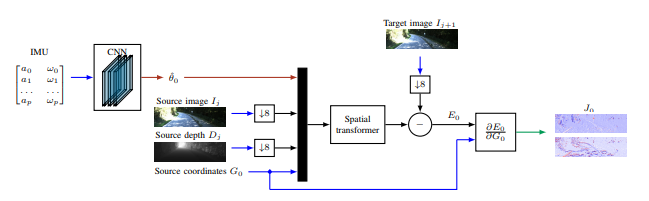
\includegraphics[width=0.90\textwidth]{thesis_template/img/unsupervised_VIO.png}
   \caption{Architecture for the first processing unit from \cite{DBLP:journals/corr/abs-1803-05850}. This unit receives the windowed IMU data as input and using a CNN outputs an affine transformation matrix estimate. 
   This transformation is applied to the initial image frame and subtracted pixel-wise from the next image frame.
   Finally, the jacobian matrix of the pixel difference derivative with respect to the initial state is computed, and fed to the next unit of this prediction system (not included in this figure).}
   \label{fig:first_unit_unsupervised_vio}
\end{figure}
\chapter{Methods}\label{chap:methods}

As we reviewed in Chapter \ref{chap:introduction}, so far the problem of IO and especially on 3D datasets is largely unexplored.
In this project we study several approaches at DL using inertial datasets for the task of IO.
Some of these approaches are inspired from the existing literature, and some of them are original of this work.
In this second chapter, we will discuss the different DL training pipelines that we studied and trained, and what knowledge we got from their results.
The aim of this section is to provide logically structured information about our findings during our  iterative succession of experiments and discoveries.
We will therefore be making special focus on the mathematical reasoning behind our decisions, and how each one is followed by the next generation of deep models.
As such, some results of these experiments will be provided in this chapter whenever they are useful to justify a decision, but Chapter \ref{chap:experiments} will be the one focused on this purpose.

As we showed during the state-of-the-art review in Section \ref{sec:related_work}, there is still no standardized pipeline on how to work with windows of inertial data. 
By far, the two most used approaches were CNN's and LSTM's but, to the best of our knowledge, none of the studies managed to proof that one was rigorously better than the other. 
Only \cite{DBLP:journals/corr/abs-1802-02209} did an empirical comparison between both, and in their results it was only shown that LSTM-based architectures were training faster (in terms of loss function reduction per epoch), but really no specifications about the CNN architectures were provided.

Because of this, and since it was is also the simplest of all the studied approaches, we begin by reproducing and adapting the work of \cite{DBLP:journals/corr/abs-1808-03485}, described in Section \ref{sec:speed_reg}. 

\section{First model: CNN speed regressor}

Another reason why we decide to start working with CNN's, is that they train much faster than RNN's, since for the latter the hidden state sequences cannot be computed in parallel. 
We transcribe the CNN model from the open source Torch code in \cite{DBLP:journals/corr/abs-1808-03485} to Tensorflow 2.0a, and train it using windows of 200 samples of IMU data, as described in the original article. 
To increase the amount of training data and to enforce shift-invariant feature extractions, we use an overlap of $w-1$ in between two windows of data (i.e., we generate one new training sample for each IMU recording, so that all the previous samples are shifted by one position in time).

We also modify the original structure shown in Figure \ref{fig:speed_net} of the model by adding a MaxPooling layer between the convolution block and the dense block (even though in the paper they explicitly specify that they didn't use them).
\begin{figure}[h]
   \centering
   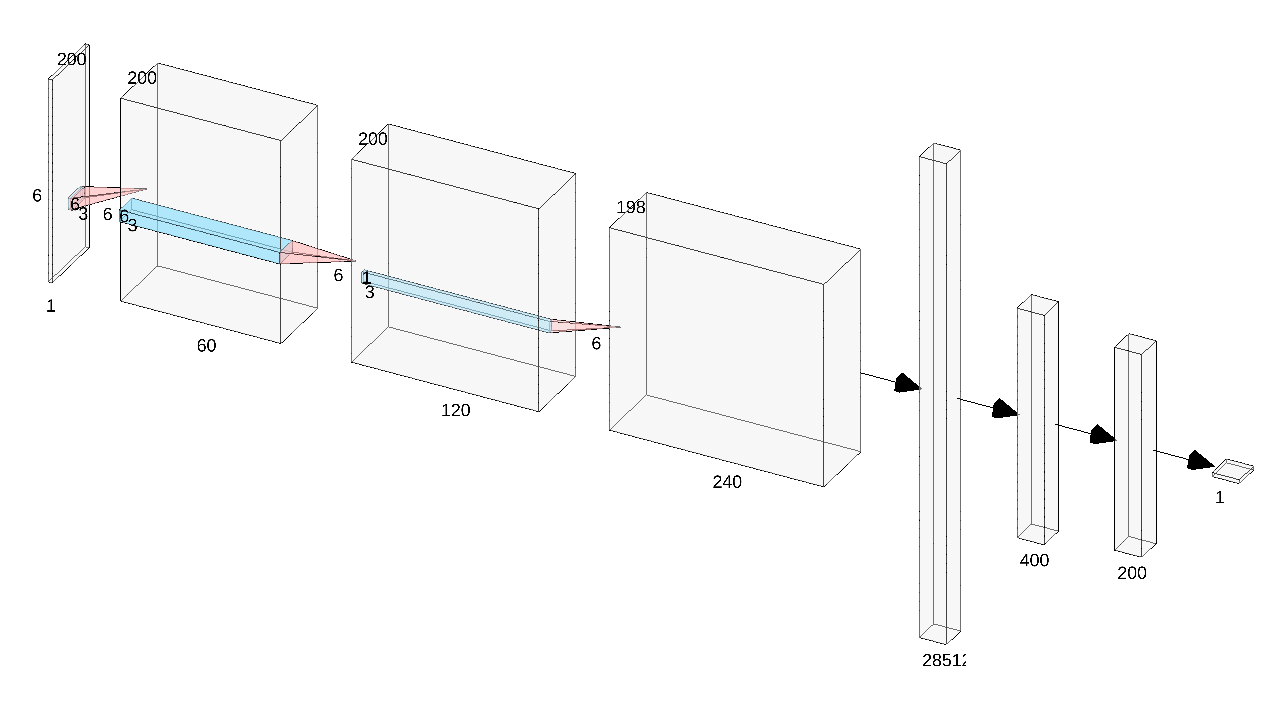
\includegraphics[width=0.75\textwidth]{img/speed_net.png}
   \caption{CNN architecture used for the speed regression task, adapted from \cite{DBLP:journals/corr/abs-1802-02209} (the dimensions of the blocks are not in scale).
   The input of this network is a window of IMU measurements, and the output corresponds to the speed (velocity norm) estimate for the time sample corresponding to the last time sample of this window.}
   \label{fig:speed_net}
\end{figure}

We make this design choice in order to reduce the number of parameters used by the architecture, as this number heavily depends on the size of the input IMU matrix $\mathbf{\hat{M}}$.
In fact, even after applying the pooling, the total number of trainable weights of the model is more than 18 million, where most of them come from the connection between the flattened convolutional feature vector and the first dense layer.

After some necessary pre-processing of the dataset which will be discussed next, the model is able to fit the training data accurately.
Unfortunately however, it is not able to successfully regress the drone speed on data from different validation sets (see Figure \ref{fig:speed_prediction_train_and_val}).
In fact, the training of this model took 150 epochs, at which point it was interrupted because the validation accuracy stopped improving.
We also left the model continue training, and eventually it could fit almost perfectly the training data around epoch 180, but no significant improvement would occur on the validation set.

\begin{figure}[h]
   \centering
   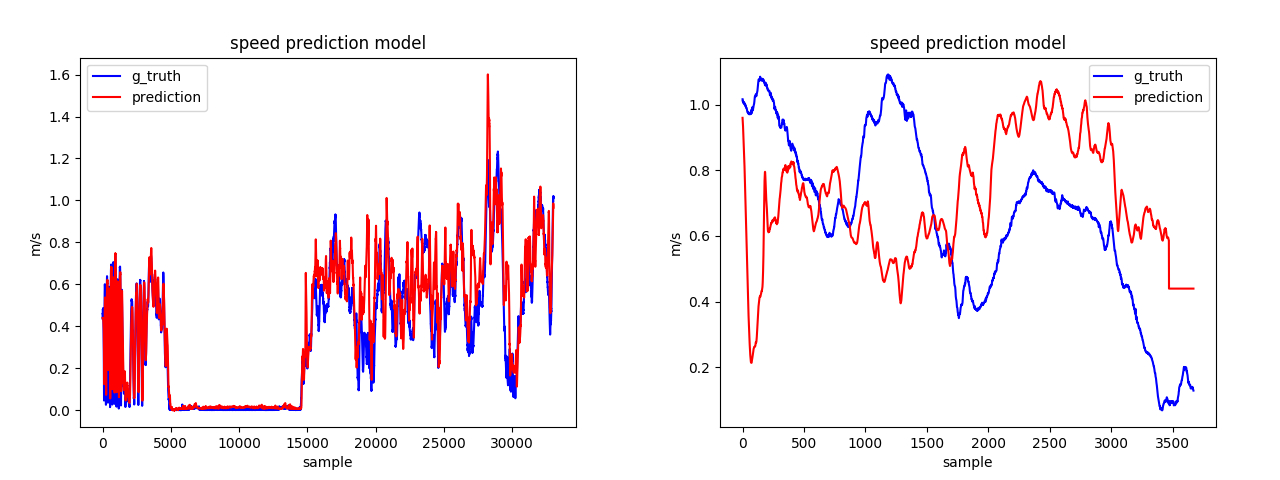
\includegraphics[width=0.90\textwidth]{thesis_template/img/speed_prediction_training_and_validation.jpg}
   \caption{Prediction of the speed regression model on the training (left) and testing (right) EuRoC dataset. Although the former prediction is accurate, it is clear that the model is failing for the validation set.}
   \label{fig:speed_prediction_train_and_val}
\end{figure}

Such fact leads us to the hypothesis that the model is heavily over-parametrized for the simplicity of its output, and it has in fact overfit a mapping between IMU readings and output speed in the training set. 
Moreover, as pointed out by \cite{DBLP:journals/corr/abs-1802-02209}, it should not be possible to fully predict the state $\mathbf{x}(k+w)$ or any of its sub-components, without having the initial state $\mathbf{x}(k)$. 
In other words, it should not be possible for the model to learn a reliable mapping $f_\theta\left(\mathbf{\hat{M}}_k\right)\mapsto\hat{s}(k)$ for any $\theta$, unless there was some encoding of the initial state somehow in the IMU readings that we are not aware of.
Therefore, whatever this CNN model was learning to regress the speed of the drone, it is most likely just an overfit of the training data.

To test this hypothesis, we use a synthesized version of the EuRoC dataset, where noise has been completely removed from the IMU.
In particular, we take a second flight sequence (not used in training), and generate \emph{ideal} IMU data with the package\href{https://github.com/zurich-eye/ze\_oss}{Zurich Eye VI simulator}.
Then, we make predictions with the model using this dataset, surprisingly obtaining not terrible results, as shown in Figure \ref{fig:speed_prediction_ideal_filtered}.
Even though the IMU has been completely removed of its noise, and this dataset is synthetic, this result points out that maybe there is something more to learn from the state in the IMU measurements.

\begin{figure}[h]
   \centering
   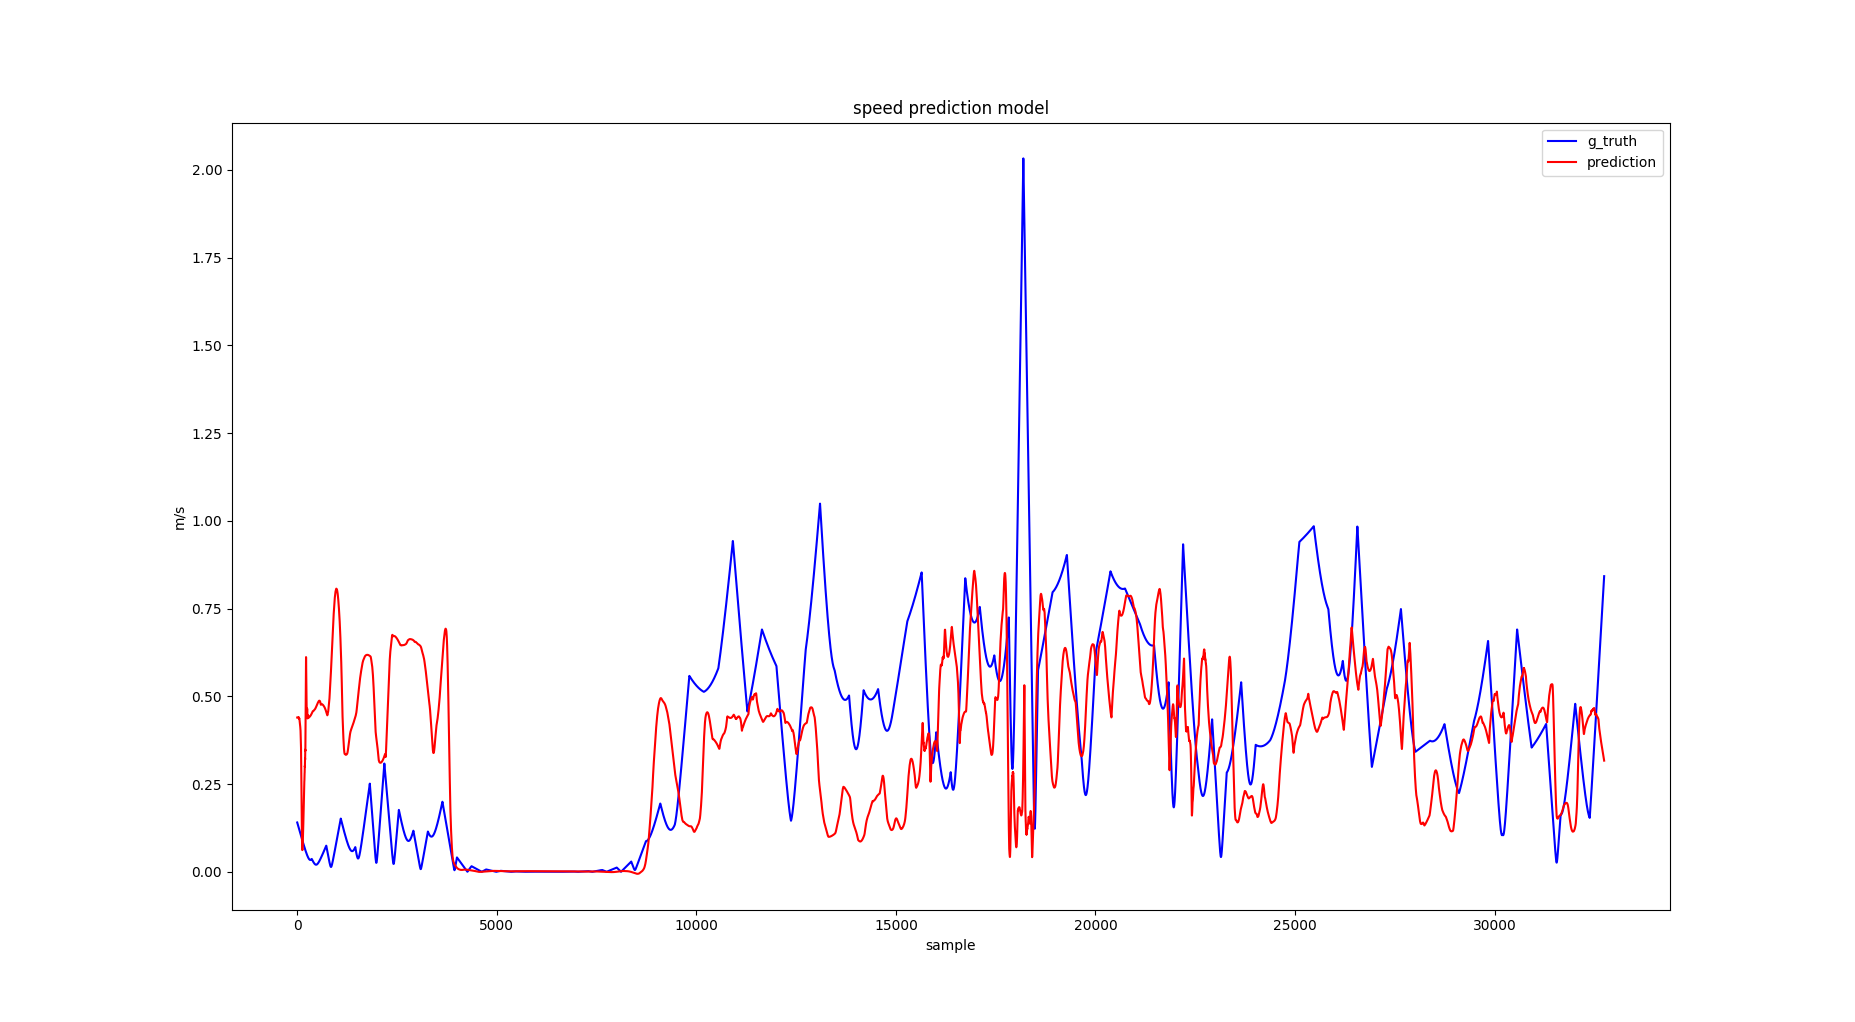
\includegraphics[width=0.85\textwidth]{thesis_template/img/ideal_filtered_speed_prediction_expandedplot.png}
   \caption{Predictions of the CNN speed regression model trained with filtered EuRoC data on a noiseless synthetic test dataset, generated from a difference sequence of the EuRoC dataset.}
   \label{fig:speed_prediction_ideal_filtered}
\end{figure}

To wrap up this first experiment, we emphasize two interesting conclusions we reach from the results:
\begin{itemize}
    \item In the original work \cite{DBLP:journals/corr/abs-1808-03485} that inspired this model, the main purpose of the authors is to train a deep regressor to provide a low-confidence speed prior for a recursive EKF pipeline, proposed in \cite{DBLP:journals/corr/SolinCRK17}. 
    We have argued why this kind of predictor will likely never be able to reliably learn a reliable encoding of the state from IMU measurements, and why the overall architecture of this model, with so many parameters, is not optimal. 
    However, as we will discuss in Section \ref{sec:pre_int_training}, it is indeed possible to learn a prior from $\mathbf{\hat{M}}_k$ that does not exactly represent the future state $\hat{s}(k)$, but can nevertheless be used to constrain it. 
    Furthermore, we have seen that, in an ideal test dataset, this model can still output a speed regression that somewhat makes sense. 
    Therefore, we leave as future work to incorporate this output, or maybe a more complex one (like a full velocity vector $\mathbf{\hat{v}}$), as an observation update to an EKF ogr similar state estimation algorithm.
    \item Despite that we will move on to a second kind of task in the incoming Section \ref{sec:imu_state_int}, we did gain some important knowledge with this first model and task about how to pre-process the inertial data, which we discuss in the appendix, in Section \ref{sec:euroc_filtering}.
\end{itemize}


\section{Second model: IMU state integrator}\label{sec:imu_state_int}

From the knowledge gathered during the previous model iteration, we set ourselves a new objective: train a model to perform noise-reduced IMU integration. 
In other words, we want to train a model that somehow learns to filter out the noise from $\mathbf{\hat{M}}_k$, and then use that to perform IMU integration.
In order to do this, we clearly learned in Section \ref{sec:speed_reg} that we require, besides the IMU data itself, to input the initial state $\mathbf{x}(k-w)$ to the model, as otherwise trying to predict $\mathbf{x}(k)$ is not mathematically feasible.
Put in equation form, for this task we want to train a deep regressor that performs the mapping \ref{eq:state_integration_problem}.
\begin{equation}\label{eq:state_integration_problem}
    f_\theta\left(\mathbf{x}(k-w),\mathbf{\hat{M}}_k\right)\mapsto\mathbf{\hat{x}}(k), \;\;\; \mathbf{x}(k)=\begin{pmatrix}\mathbf{p}\\ \mathbf{v}\\ \mathbf{q}\end{pmatrix}\in \mathbb{R}^{10}
\end{equation}
Where $\mathbf{p}, \mathbf{v}\in\mathbb{R}^3$ represent the $(x,y,z)$ position and velocity vectors in Euclidean space, and $\mathbf{q}\in\mathbb{Q}^4$ represents the unitary quaternion describing the rotation from the inertial frame $W$ to the body frame $B$. 
In other words, $\mathbf{q}$ is the unit quaternion form of the rotation matrix $\mathbf{R}_{W\!B}\in SO(3)$.
Notice that the members of the unitary rotation quaternion group $\mathbb{Q}^4$, although having 4 components, only three of them are independent.

To the best of our knowledge, this task had not been performed with a deep model in the literature yet in a 3-dimensional setup.
Consequently, we could not use any NN architecture as a foundation, so we designed our own model with the mathematical graph flow of IMU integration in mind.
Furthermore, since we verified that convolutional layers were indeed being able to generate a meaningful representation of $\mathbf{\hat{M}}_k$ in Section \ref{sec:speed_reg}, we used them once again to process the IMU data during the first layers of the model. 
The first architecture iteration for this task is shown in Figure \ref{fig:state_int_v0}.

\begin{figure}
    \centering
    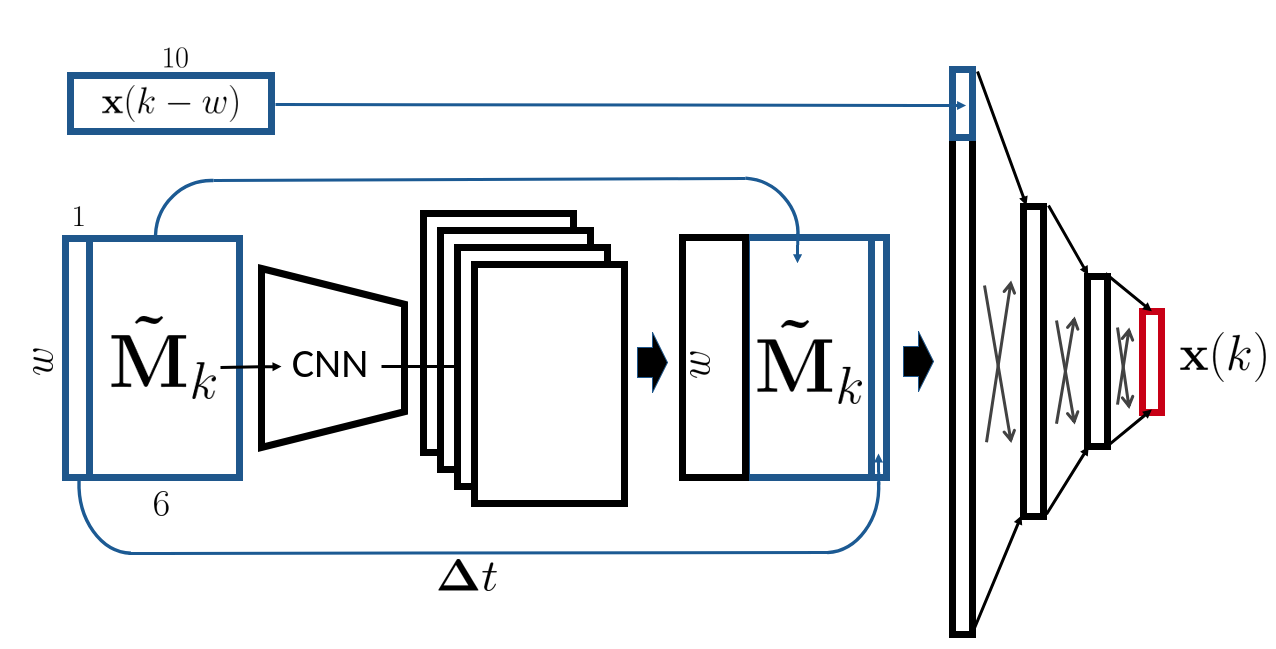
\includegraphics[width=\textwidth,height=\textheight,keepaspectratio]{thesis_template/img/imu_int_net.png} 
    \caption{Schematic architecture of IMU integration network. The IMU measurement matrix $\mathbf{\hat{M}}_k$ is processed by a series of convolutional layers, and the resulting generated feature vector is concatenated with the original $\mathbf{\hat{M}}_k$, and the $\Delta t$ vector, which contains the time difference between consecutive measurements.
    The concatenated tensor is then fed through one more convolutional layer, flattened, and appended to the initial state $x(k-w)$.
    Finally, three dense layers are applied, which output the predicted state $\mathbf{\hat{x}}(k)$}
    \label{fig:state_int_v0}
\end{figure}

The intuition behind the architecture is the following: with the convolutional block, we extract features from $\mathbf{\hat{M}}_k$. 
The convolution layers are designed so that gyroscope and accelerometer readings are not convolved together (by using the right kernel sizes and strides), as they physically represent different things. 
Also, besides using less channels than before in Figure \ref{fig:speed_net}, we add one extra convolutional layer that summarizes the channel dimension to only 5 components, to reduce the number of parameters needed for the final dense layers.
Then, this feature vector is concatenated with the original $\mathbf{\hat{M}}_k$ and the $\boldsymbol{\Delta}\mathbf{t}$ vector (which is a $w\times 1$ vector containing the time difference between two consecutive readings) and a final convolutional layer is applied.
The kernel of this layer is designed to occupy the entire length of the joint matrix, with the hope that it will learn to integrate the $\boldsymbol{\Delta} t$ into the system.

Finally, the resulting tensor is flattened, concatenated with the initial state, and fed into a sequence of Dense layers with ReLU activation, with the final layer outputting a 10-dimensional vector, as in \ref{eq:state_integration_problem}.
The last dense layer does not use any activation function. 
We decided to concatenate the convolutional feature vector with the original IMU matrix $\mathbf{\tilde{M}}_k$ for debugging purposes in later stages; i.e. to see whether the network was actually taking advantage of the convolutional layers.
This network has a total of 440K trainable parameters, and one epoch is trained in around 12 seconds in an i7 CPU. 

For this task, we investigate a second MAV dataset: MIT's BlackBird (BB) \cite{antonini2018blackbird}.
Compared to EuRoC dataset, the BB dataset has higher frequency ground truth annotations, more recorded sequences (a total of over 10h and 60km of data) and also more aggressive motion, with a top speed of up to 7m/s. 
By contrast, EuRoC reaches a top speed of 2.3m/s.

\subsection{First Iteration}
For the first iteration of this task, we train the model described in Figure \ref{fig:state_int_v0} with a smaller IMU window than last time: $w=50$. 
In the BB dataset, which uses an IMU that measures at 100Hz, this represents a 0.5s time interval.
The optimal parameters $\theta^*$ for this model are also recovered using the backpropagation algorithm with an Adam optimizer. 
The loss function chosen to be minimized during this training is defined by \ref{eq:q_state_loss}.
\begin{equation}\label{eq:q_state_loss}
    \mathcal{L}= \sum{\left \|\mathbf{p}-\mathbf{\hat{p}}  \right \|_2^2} + \sum{\left\|\mathbf{v}-\mathbf{\hat{v}}  \right \|_2^2} + \left |\sin\left(\left(\mathbf{q}^{-1}\mathbf{\hat{q}}\right)_\measuredangle \right)  \right |.
\end{equation}
Where $\mathbf{q}^{-1}\mathbf{\hat{q}}$ computes the quaternion that rotates $\mathbf{q}$ to $\mathbf{\hat{q}}$, and the operator $\measuredangle$ represents its angle.
The $|\sin(\cdot)|$ operation is then used to compensate for the periodicity of the angle error.

As a proof of concept, this model was trained on one of the easiest flights in the dataset: the flight sequence \emph{Thrice} (which barely has any motion in the z axis) and with a maximum speed of 2m/s.
However, to test better the model, it was validated on the sequence \emph{BentDice}, which is a flight sequence with a lot more of z displacement. 
Additionally, the predictions were compared with manual IMU double integration as a baseline.

The results of this experiment reveal that the model outperforms double integration for predicting the $\mathbf{v}$ vector, and the x and y components of the $\mathbf{p}$ vector.
On the other hand, it is not quite reaching this baseline for the z elevation coordinate, which was expected as the training dataset was flat, or the rotation term $\mathbf{q}$.
Figure \ref{fig:imu_int_50} depicts such results.
The horizontal axis corresponds to one sample of the test dataset; i.e., for each sample $k$ the input to both the model and the double integration algorithm is $(\mathbf{x}(k-w), \mathbf{\hat{M}}_k)$ and the optimal output to be obtained is the ground truth in blue, representing $\mathbf{x}(k)$.
\begin{figure}
    \centering
    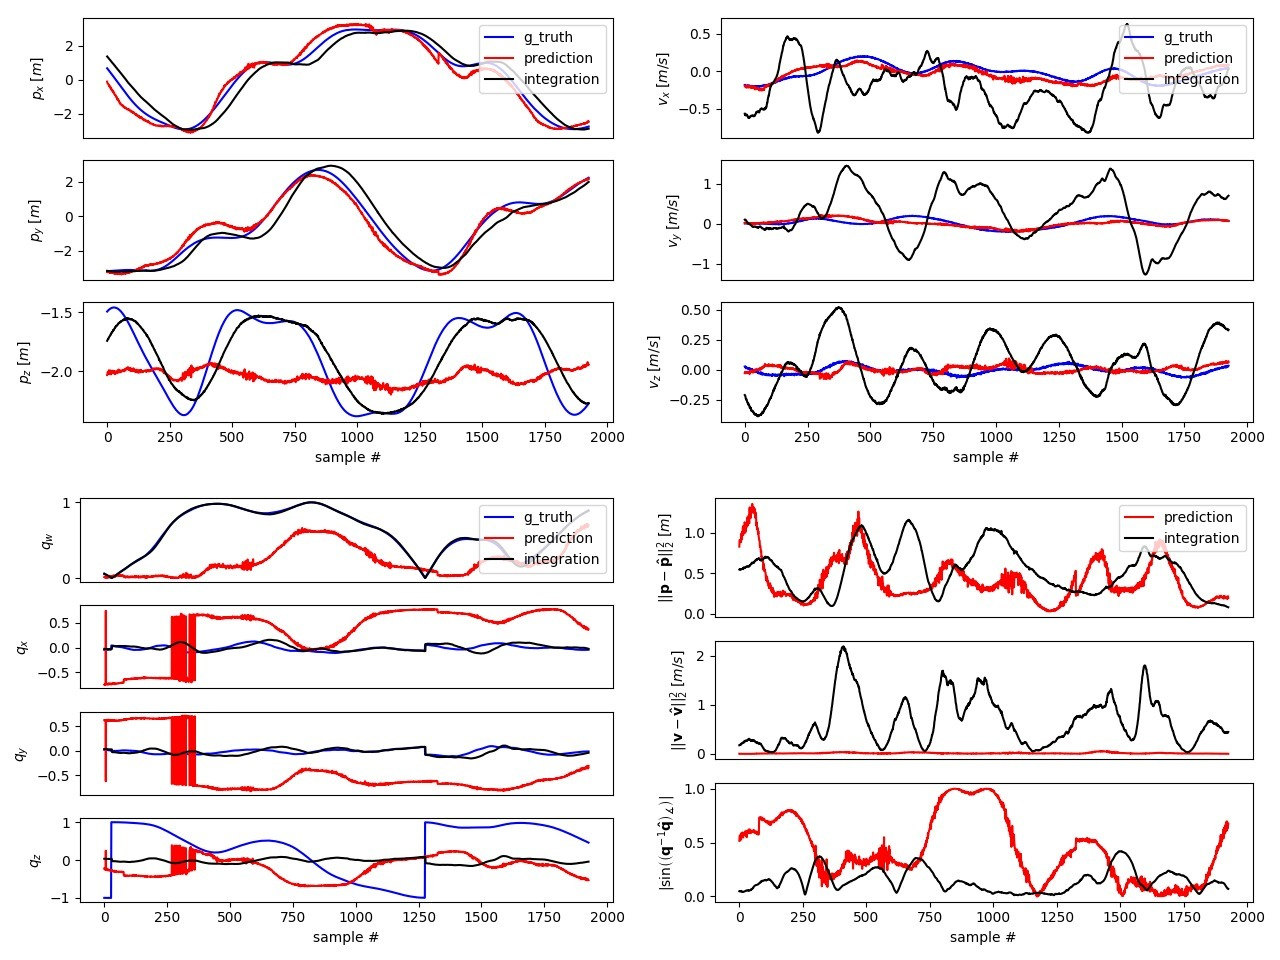
\includegraphics[width=\textwidth,height=\textheight,keepaspectratio]{thesis_template/img/imu_int_50.jpg} 
    \caption{Comparison between ground truth, model predictions and IMU double integration in set-aside validation set from the Blackbird \emph{bentDice}@2m/s sequence. For each x-axis entry, the inputs to the model and the double integration algorithm are the initial ground truth state $\mathbf{x}(k-w)$, and the output is the predicted state $\mathbf{x}(k)$. 
    The bottom right plot shows the error of both algorithms compared to the ground truth computed by the loss function \ref{eq:q_state_loss}.}
    \label{fig:imu_int_50}
\end{figure}

After inspection of this first test, we point out three main issues with this approach, for which we propose solutions in Sections \ref{sec:lie_algebra} and \ref{sec:pre_int_training}.
\begin{enumerate}
    \item \label{item:quaternion_loss_problem} The loss function \ref{eq:q_state_loss} for the rotation term is highly nonlinear, and the model cannot learn how to predict $\mathbf{q}$ properly. 
    This is probably because the constraint for the quaternion to be unitary creates nonlinear dependencies between the quaternion terms.
    In fact, the model showed to have serious problems even at fitting this distribution in the training set.
    \item \label{item:input_state_problem} Contradicting our own statement in the first paragraph of this section, the input state $\mathbf{x}(k-w)$ should \emph{not} be an input to the system.
    This is because if we feed $\mathbf{x}(k-w)$ to the deep model, and if the window of time corresponding to $w$ is small enough (in our case 0.5s), the model can learn an \emph{easy mapping} between $\mathbf{x}(k-w)$ and $\mathbf{x}(k)$ by not changing the input state.
    In other words, the initial state is necessary for performing IMU integration, but the model cannot rely on it to learn.
    \item Linked with problem \ref{item:input_state_problem}, in order to properly learn IMU integration in this setup it would be necessary to augment our dataset infinitely in order to make the model learn how to use the IMU data.
    This is because there are infinitely many initial and final position and velocity configurations.
\end{enumerate}

\subsection{Iteration 2: improved rotation loss term}\label{sec:lie_algebra}

In order to solve problem \ref{item:quaternion_loss_problem}, we draw inspiration from the approach proposed in \cite{DBLP:journals/corr/ClarkWWMT17} to enable a deep model to output in $SE(3)$ space (the general overview was discussed in Section \ref{sec:VIOnet}).
In the original work, the authors want to train a model to predict a series of homogeneous transformation matrices $\mathbf{T}$ from visual and inertial inputs. 
The definition of $\mathbf{T}$ is given by \ref{eq:homog_transf}. 
\begin{equation}\label{eq:homog_transf}
    _{W}\mathbf{T}_{AB}=\left\{\begin{pmatrix}_{W}\mathbf{R}_{AB}&_W\mathbf{t}_{AB}\\\mathbf{0}&1\end{pmatrix}\bigg\rvert\; _{W}\mathbf{R}_{AB}\in SO(3),\; _{W}\mathbf{t}_{AB}\in \mathbb{R}^3\right\}\in SE(3).
\end{equation}
Unfortunately, the special group $SO(3)$ is subject to orthogonality constraints, which are hard to figure out by a deep model.
This phenomenon is similar to what we are experimenting with the quaternion representation of rotation in $\mathbb{Q}^4$.

(\emph{All the algebra derivations that will follow are adaptations of chapter 8 of \cite{se3_tutorial}}).
On the other hand, the $SO(3)$ manifold is a subset of the invertible 
$3\!\times\!3$ matrices group $\mathbf{GL}(3, \mathbb{R})$. 
Any subgroup $G \in \mathbf{GL}(3, \mathbb{R})$ has two interesting properties:
\begin{enumerate}
    \item\label{item:G_linear_lie} $G$ is a linear Lie group.
    \item Derivable from property \ref{item:G_linear_lie}, the set $\mathfrak{g}$ in \ref{eq:lie_algebra_group}
    \begin{equation}\label{eq:lie_algebra_group}
    \mathfrak{g}=\left\{\mathbf{X}\in M (3,\mathbb{R})\rvert e^{t\mathbf{X}}\in G, \forall t \in \mathbb{R}\right\}.
    \end{equation}
    is a vector space tangent to $G$ at the identity $I$, and is closed under the Lie bracket operator, where $ M (3,\mathbb{R}):=\mathbb{R}^{3\!\times\! 3} \;\; s.t. \; \mathbf{GL}(3, \mathbb{R})\subset M (3,\mathbb{R})$.
\end{enumerate}

Effectively, this means that the matrix exponential operation $e^\mathbf{M}$, which has a convergent power series form denoted by \ref{eq:mat_power}, when $\mathbf{M}\in SO(3)$, computes its tangent vector space, which is an Euclidean space.
\begin{equation}\label{eq:mat_power}
    e^ M =\sum_{k=0}^{\infty }\frac{1}{k!} M ^k
\end{equation}
It so happens that the tangent space at of a Lie group $ M $ at its identity is also its lie algebra $\mathfrak{m}$ by definition.
Furthermore, there are two operations that relate the general Lie group $ M $ and its Lie algebra $\mathfrak{m}$:
\begin{itemize}
    \item The exponential map $\textrm{exp}:\mathfrak{m}\mapsto M $
    \item The logarithmic map $\textrm{log}: M \mapsto\mathfrak{m}$
\end{itemize}

For the case of the $SO(3)$ group, the corresponding Lie algebra is denoted by $\mathfrak{so}(3)$, and its base are three skew symmetric matrices corresponding to infinitesimal rotations along different axis.
Skew symmetric matrices in $\mathbb{R}^{3\!\times\!3}$ only have three independent components, and so can be perfectly mapped to a vector in $\mathbb{R}^3$ and \emph{vice versa} with the \emph{hat} $(\cdot)^{\wedge}$ and \emph{vee} $(\cdot)^{\vee}$ operators, as shown in \ref{eq:hat_and_vee}.
\begin{equation}\label{eq:hat_and_vee}
    \boldsymbol{\omega}=\begin{bmatrix}x\\y\\z\end{bmatrix}\rule{1cm}{0cm}\;
    \boldsymbol{\omega}^{\wedge}=\begin{pmatrix}0&-z&y\\z&0&-x\\-y&x&0\\\end{pmatrix}\rule{1cm}{0cm}\;
    ({\boldsymbol{\omega}}^\wedge)^\vee=\boldsymbol{\omega}.
\end{equation}
Finally, there are also specific exponential and logarithmic mappings that allow to map a rotation quaternion in $\mathbb{Q}^4$ to $\mathfrak{so}(3)$ and back, which have the forms \ref{eq:q_exp_map} and \ref{eq:q_log_map} respectively.
\begin{equation}\label{eq:q_exp_map}
    \mathbf{q}\doteq e_q^{\boldsymbol{\omega}}=\left\{ 
	\begin{array}{ll}
		(1,0,0,0)^\top  & \text{ , if }  \boldsymbol{\omega} = (0,0,0)^\top \\
		\left( \cos\dfrac{|\boldsymbol{\omega}|}{2}, \dfrac{\sin\dfrac{|\boldsymbol{\omega}|}{2}}{|\boldsymbol{\omega}|} ~ \boldsymbol{\omega} \right)^\top &  \text{ , otherwise}
	\end{array}
	\right.
\end{equation}
\begin{equation}\label{eq:q_log_map}
    \mathfrak{q}\doteq\boldsymbol{\omega}=\frac{2\arccos(q_r)}{|\mathbf{q}_v|}\mathbf{q}_v
\end{equation}

Recapitulating where we left off before this derivation, in \cite{DBLP:journals/corr/ClarkWWMT17} the authors want to train a model to output in $SE(3)$ space.
This was problematic because the $SO(3)$ rotation matrix in $SE(3)$ is subject to nonlinear constraints, which render any loss function to treat it very non-convex.
As a solution, they propose that the model predicts instead of the $SE(3)$ matrix, the Lie algebra representation of $\mathbf{T}$, whose rotation term in $\mathfrak{so}(3)$ can be expressed as a 3-component vector without any orthogonality constraints.
This makes the loss function significantly less nonlinear than when trying to work in $SO(3)$.

In our case, by adopting this idea, we train the deep model so it learns to predict the $\mathfrak{so}(3)$ representation of the rotation produced during a time sequence of length $w$.
This prediction is then manually remapped to $\mathbb{Q}^4$ with a final, non-trainable layer, in order to output a state with the same form as the initial state, as described in \ref{eq:state_integration_problem}. 
However, to simplify notation, we will state that the model now performs the mapping \ref{eq:state_integration_problem_so3}:
\begin{equation}\label{eq:state_integration_problem_so3}
    f_\theta\left(\mathbf{x}(k-w),\mathbf{\hat{M}}_k\right)\mapsto\mathbf{\hat{x}}(k), \;\;\;
    \mathbf{x}(k)=\begin{pmatrix}\mathbf{p}\\ \mathbf{v}\\ \mathbf{q}\end{pmatrix}\in \mathbb{R}^{10},\;\;
    \mathbf{\hat{x}}(k)=\begin{pmatrix}\mathbf{\hat{p}}\\ \mathbf{\hat{v}}\\ \mathfrak{\hat{q}}\end{pmatrix}\in \mathbb{R}^{9}
\end{equation}
And with this formulation, the new loss function becomes \ref{eq:state_so3_loss}, where the rotation term has changed with respect to \ref{eq:q_state_loss}.
\begin{equation}\label{eq:state_so3_loss}
    \mathcal{L}= \left \|\mathbf{p}-\mathbf{\hat{p}}  \right \|_2^2 + \left\|\mathbf{v}-\mathbf{\hat{v}}  \right \|_2^2 + \left\|\textrm{log}\left(\mathbf{q}\right)-\mathfrak{\hat{q}}\right\|_2^2.
\end{equation}
Where $\textrm{log}(\mathbf{q})$ is the $\mathfrak{so}(3)$ representation via the logarithmic mapping \ref{eq:q_log_map} of $\mathbf{q}$.

From the architecture point of view, the change in the rotation prediction type only affects to the final layer of the network model, which instead of having a 10 unit dense layer, now its 9 units, so that the new model now performs the mapping \ref{eq:state_integration_problem_so3}.

After applying these changes we train the model this time on the 3D sequence \emph{bentDice}, i.e. the one that we used for validation in the previous iteration of the model.
First, we check that with the new formulation, the model is indeed able to fit in the rotation quaternion, as now it does not have the extra imposed constraint of the rotation being unitary.
We set aside a segment of the \emph{bentDice} sequence, which was not used for training, and use it as validation set.
Figure \ref{fig:so3_rotation_fit} demonstrates that the model performs quite good on this experiment.
Even more interestingly, we can see how the model appears even to be adapting to the sign flips of the rotation axes in the left figure.
This is interesting albeit not ideal, as this is also a form of added difficulty that the model has to overcome to perform well on the task. 
We will tackle this issue too in the next section.
\begin{figure}
    \centering
    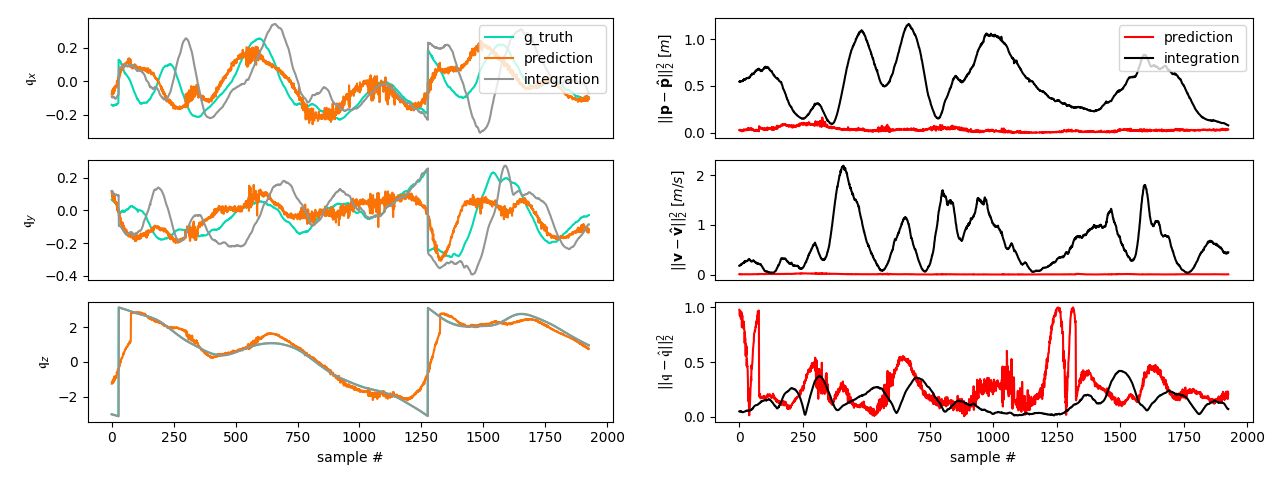
\includegraphics[width=\textwidth,height=\textheight,keepaspectratio]{thesis_template/img/imu_int_so3_rot_fit.jpg}
    \caption{Rotation predictions in Lie Algebra space in set-aside set from BB \emph{bentDice}@2m/s. The left plot shows the predictions of the three components of rotation state.
    The right are the losses (errors) for position, velocity and rotation for both the predicted and integrated states.
    The model is able to fit in the $\mathfrak{so}(3)$ rotation term, and this helps also to improve the position and velocity estimates, so that this model is constantly outperforming double-integration for the full state vector. }
    \label{fig:so3_rotation_fit}
\end{figure}

For the next experiment, we select a completely new validation dataset from the BB set, also rich in 3D motion, and also significantly more aggressive (with maximum speeds of 6m/s). 
We repeat the experiment, and summarize the results in Figure \ref{fig:so3_tiltedThrice_fit}.
Even though the predictions are good for $\mathbf{v}$ and for the $p_x$ and $p_y$, the model under-performs once again for the $\mathbf{q}$ term, and achieves a similar performance than integration for $p_z$. 
By closer inspection, it can be seen that this dataset is very rich in rotation axes sign flips, which is very likely to be the cause of the problem with the rotation fit, as we pointed out earlier. 
\begin{figure}
    \centering
    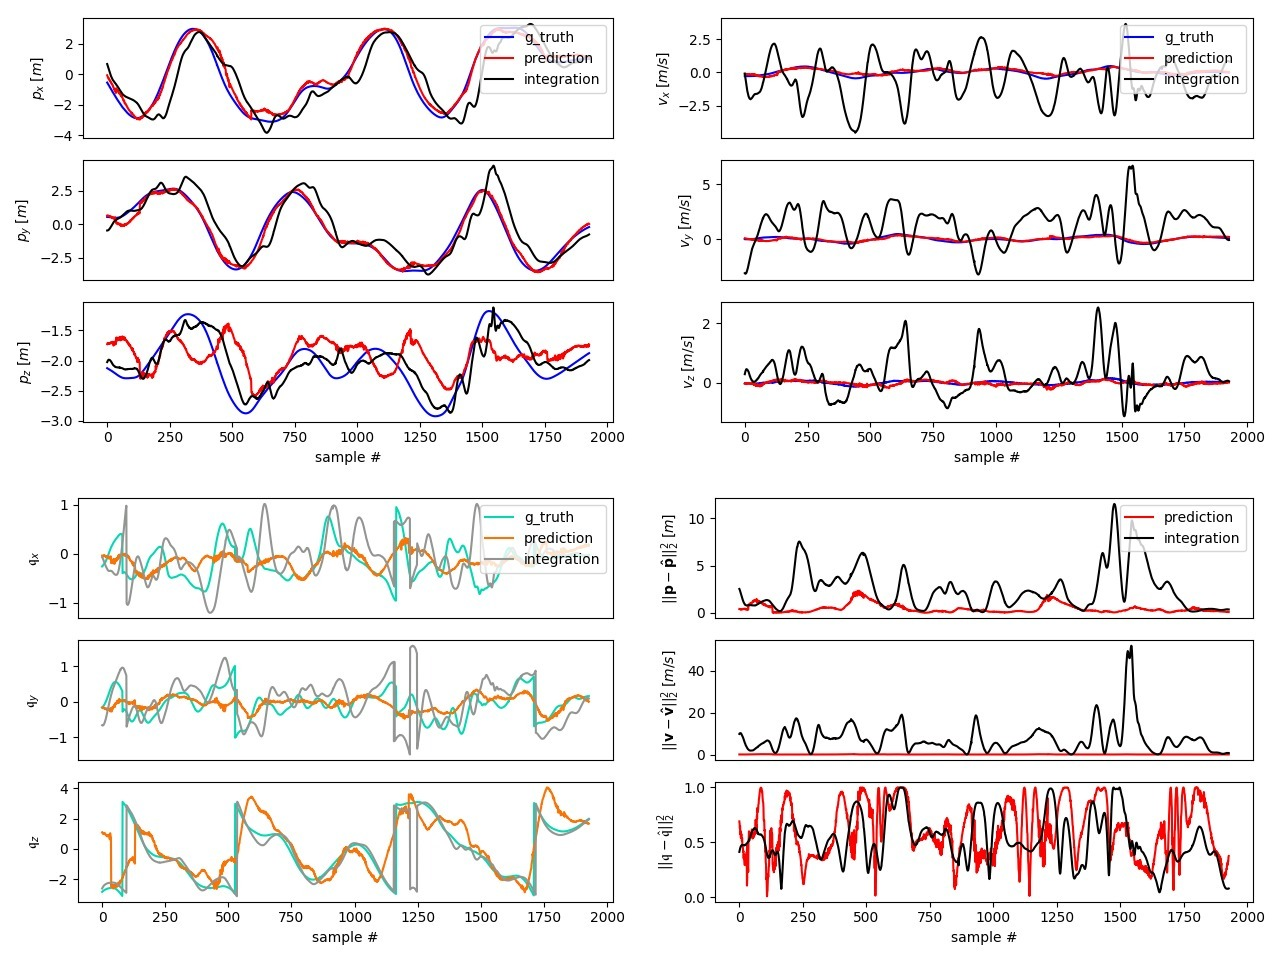
\includegraphics[width=\textwidth,height=\textheight,keepaspectratio]{thesis_template/img/imu_int_50_so3_tiltedThrice.jpg}
    \caption{Full comparison between ground truth, predicted and double-integrated states from IMU data. 
    The experiment is performed on the much more aggressive \emph{tiltedThrice}@6m/s BB sequence. 
    The bottom right plot again corresponds to the losses for the $\mathbf{p}$, $\mathbf{v}$ and $\mathfrak{q}$ terms, computed from \ref{eq:state_so3_loss}
    The model is unable to perform well the iterative task (right) on the training set
    $\mathbf{p}$ and $\mathbf{v}$ but both fail again in the rotation term.}
    \label{fig:so3_tiltedThrice_fit}
\end{figure}

For the final experiment round of this iteration, we set up a pipeline where the model prediction is fed back as input, together with the next sequence of IMU measurements, and repeat over a sequence of time. 
We refer to this test as the \emph{iterative} experiment in \ref{chap:experiments}. 
As a sanity check, this iterative experiment is first performed on the training dataset.
Unfortunately, despite that, the deep model is unable to successfully recover the trajectory using the iterative method, as shown in Figure \ref{fig:iterative_exp_fail}.
On the left plot, the 3D view of the predicted trajectory is plotted when the ground truth is fed to the model every $w$ time samples.
On the right, the model uses its own past prediction as new input in an iterative manner, every $w$ samples.
\begin{figure}
    \centering
    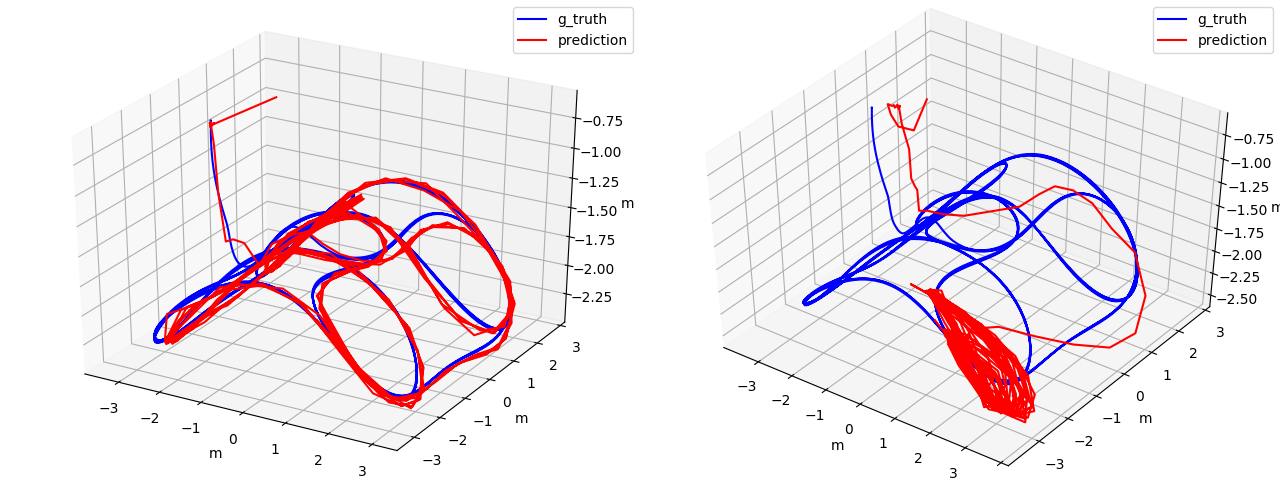
\includegraphics[width=\textwidth,height=\textheight,keepaspectratio]{thesis_template/img/iterative_exp_vs_gt.png}
    \caption{Left figure: prediction of the state integrator model on the training dataset. Right figure: prediction of the state integrator model on the training dataset, but only the first state is provided as input, instead of a state for every $\mathbf{\hat{M}}_k$.}
    \label{fig:iterative_exp_fail}
\end{figure}

This result yields to the conclusion that the model is too dependent on the initial state input of the system, and really is not learning IMU integration as well as originally thought. 
In section \ref{sec:exp_imu_int_so3} we perform a more in-depth analysis of what is going on, and conclude that, although the model learns some notion about integrating the IMU in the x and y axes, the architecture of this model is not optimal for learning this task.
We also conclude, however, than CNN layers are actually useful to process the IMU data.

In next section, we present a new approach to learn from inertial data for state integration in the next section, where the initial state is still fed to the model, but the model is prevented from learn from it.
The architecture that will be used implicitly enforces to learn the IMU integration task, while filtering the noise of the IMU at the same time.

\section{Third model: IMU pre-integration}\label{sec:pre_int_training}

As concluded in the literature review, feeding the initial state to the deep model is dangerous as it may up learning a mapping between initial state and final state.
Although in the experiments chapter we show that this is particularly not the main problem with the model proposed in Section \ref{sec:exp_imu_int_so3}, it is an issue worth finding a solution for.
This is especially the case when we use short values of $w$, as both input and output states will be similar.

To solve this, we draw inspiration once again from \cite{DBLP:journals/corr/abs-1802-02209}, which was discussed thoroughly in Section \ref{sec:ionet}.
In particular, in this work the authors train a deep model to predict 2D state increments, in the form $\Delta\mathbf{\hat{x}}=(\Delta\hat{l}, \Delta\hat{\psi})$, by demonstrating that it is possible to mathematically calculate these state increments just with the initial velocity, gravity vector, and IMU measurements (all of them in body frame).

We adopt the idea of calculating the state increments instead of the final state just from IMU data, as this will prevent over-fitting a mapping between initial and final states.
Furthermore, the span of the manifold of IMU data is arguably much more constrained than the span of the state vector.
In other words, it could be expected for the state position $\mathbf{p}$ to be arbitrarily large or small (as long as it is in $\mathbb{R}^3$), but the IMU data will likely never contain arbitrarily large angular speeds of accelerations, as it would not be feasible for the agent to move that fast.
This fact drastically reduces the amount of training examples this model would require to learn the task

We formulate a new problem setup in full 3D space by means of the work from Forster and his team, where they introduce the \emph{IMU pre-integration} theory for the first time \cite{DBLP:journals/corr/ForsterCDS15}.
We start by defining some notation:
\begin{enumerate}
    \item $\mathbf{R}_{WB}\mapsto \mathbf{R}\doteq$ rotation from world ($W$) frame to IMU ($B$) frame in $SO(3)$.
    \item\label{lab:w_frame} $_W\mathbf{x}\mapsto\mathbf{x} \doteq$ any vector in $\mathbb{R}^3$ with physical meaning defined in the $W$ reference frame.
    \item $\mathbf{x}_i\doteq$ a physical property (also in $W$ frame by means of point \ref{lab:w_frame}) measured at time index $i$.
    \item $\mathbf{\tilde{x}}\doteq$ observation of physical property (\emph{note}: we change the notation from $\mathbf{\hat{x}}$ to $\mathbf{\tilde{x}}$ to be consistent with \cite{DBLP:journals/corr/ForsterCDS15}).
    \item $\Delta\mathbf{x}_{ij}\doteq$ change of $\mathbf{x}$ between time indices $i$ and $j$, separated by a window $w$. We refer to $i$ and $j$ as the \emph{keyframe} indices.
    \item $\Delta\mathbf{\tilde{x}}_{ij}\doteq$ pre-integrated property between time indices $i$ and $j$ with IMU data.
\end{enumerate}
Furthermore, we will assume that the state of an agent at a specific time $i$ is given by the vector $(\mathbf{p}_i, \mathbf{v}_i, \mathbf{R}_i)^T$.
From vanilla IMU double integration, the final state given the initial state and IMU measurements is calculated by \ref{eq:imu_integration}:
\begin{eqnarray}\label{eq:imu_integration}
    \mathbf{R}_j & = & \mathbf{R}_i\prod_{k=i}^{j-1}\textrm{Exp}\left(\left(\tilde{\boldsymbol{\omega}}_k -\mathbf{b}^g_k - \boldsymbol\eta^g_k\right )\Delta t \right ) \nonumber\\
    \mathbf{v}_j & = & \mathbf{v}_i + \mathbf{g}\sum_{k=i}^{j-1}\Delta t + \sum_{k=i}^{j-1}\mathbf{R}_k\left(\tilde{\boldsymbol{a}}_k -\mathbf{b}^a_k - \boldsymbol\eta^a_k \right )\\
    \mathbf{p}_j & = & \mathbf{p}_i + \sum_{k=i}^{j-1}\left(\mathbf{v}_k\Delta t + \tfrac{1}{2}\mathbf{g}\Delta t^2 + \tfrac{1}{2}\mathbf{R}_k\left(\tilde{\boldsymbol{a}}_k -\mathbf{b}^a_k - \boldsymbol\eta^a_k \right)\Delta t^2\right)\nonumber
\end{eqnarray}
Where $\mathbf{b}^a_k$ and $\boldsymbol\eta^a_k$ are the bias and noise terms of the accelerometer $(a)$, and equivalently for the gyroscope $(g)$. We group all intermediate factors needed for integration in the variables $(\Delta\mathbf{R}_{ij},\Delta\mathbf{v}_{ij},\Delta\mathbf{p}_{ij})$, which exactly represent the state increment with the definitions \ref{eq:state_increments} (notice that $\mathbf{R}_i^T\mathbf{R}_k \doteq \Delta\mathbf{R}_{ik}$):
\begin{eqnarray}\label{eq:state_increments}
    \Delta\mathbf{R}_{ij} & = & \prod_{k=i}^{j-1}\textrm{Exp}\left(\left(\tilde{\boldsymbol{\omega}}_k -\mathbf{b}^g_k - \boldsymbol\eta^g_k\right )\Delta t \right )\nonumber\\
    \Delta\mathbf{v}_{ij} & = & \sum_{k=i}^{j-1}\mathbf{R}_i^T\mathbf{R}_k\left(\tilde{\boldsymbol{a}}_k -\mathbf{b}^a_k - \boldsymbol\eta^a_k \right )\Delta t\\
    \Delta\mathbf{p}_{ij} & = & \sum_{k=i}^{j-1}\left(\Delta\mathbf{v}_{ik}\Delta t +  \tfrac{1}{2}\mathbf{R}_i^T\mathbf{R}_k\left(\tilde{\boldsymbol{a}}_k -\mathbf{b}^a_k - \boldsymbol\eta^a_k \right)\Delta t^2\right)\nonumber
\end{eqnarray}
Such that \ref{eq:imu_integration} can be rewritten as \ref{eq:imu_integration_2}.
\begin{eqnarray}\label{eq:imu_integration_2}
    \mathbf{R}_j & = & \mathbf{R}_i\Delta\mathbf{R}_{ij}\nonumber \\
    \mathbf{v}_j & = & \mathbf{v}_i + \mathbf{g}\sum_{k=i}^{j-1}\Delta t + \mathbf{R}_i\Delta\mathbf{v}_{ij}\\
    \mathbf{p}_j & = & \mathbf{p}_i + \mathbf{v}_i\sum_{k=i}^{j-1}\Delta t +  \tfrac{1}{2}\mathbf{g}\Delta t^2 + \mathbf{R}_i\Delta\mathbf{p}_{ij} \nonumber
\end{eqnarray}
Notice that the equations in \ref{eq:state_increments} have the intermediate biases and noise terms $\mathbf{b}_k$ and $\boldsymbol{\eta}_k$ in their definitions.
In \cite{DBLP:journals/corr/ForsterCDS15}, it is assumed that the bias changes slow enough so that it remains constant between keyframes $i$ and $j$ (for that, the $w$ parameter can't be very large).
The noise terms are then isolated according to \ref{eq:pre_int_x}.
\begingroup
\setlength{\arraycolsep}{2pt} % Default value: 6pt
\renewcommand{\arraystretch}{1.8} % Default value: 1
\begin{eqnarray}
    \Delta\mathbf{R}_{ij} & = & \Delta\mathbf{\tilde{R}}_{ij}\textrm{Exp}\left(\delta\boldsymbol{\phi}_{ij}\right)
        \left\{
        \begin{array}{rll}
            \Delta\mathbf{\tilde{R}}_{ij} & \doteq  & \prod_{k=i}^{j-1}\textrm{Exp}\left(\left(\tilde{\boldsymbol{\omega}}_k -\mathbf{b}^g_k \right )\Delta t \right ) \\ 
            \delta\boldsymbol{\phi}_{ij} & \doteq  & \prod_{k=i}^{j-1}\boldsymbol\eta^g_k\Delta t
        \end{array}
        \right.
        \nonumber\\
    \Delta\mathbf{v}_{ij} & = & \Delta\mathbf{\tilde{v}}_{ij} - \delta\mathbf{v}_{ij}
        \left\{
        \begin{array}{rll}
            \Delta\mathbf{\tilde{v}}_{ij} & \doteq & \sum_{k=i}^{j-1}\Delta\mathbf{\tilde{R}}_{ik}\left(\tilde{\boldsymbol{a}}_k -\mathbf{b}^a_k\right )\Delta t\\
            -\delta\mathbf{v}_{ij} & \doteq & 
            \sum_{k=i}^{j-1}{f_{\delta\mathbf{v}}\left(\Delta\mathbf{\tilde{R}}_{ik}, \delta\boldsymbol{\phi}_{ik}, \tilde{\boldsymbol{a}}_k, \mathbf{b}^a_k\right)}
        \end{array}
        \right.
        \label{eq:pre_int_x}\\
    \Delta\mathbf{p}_{ij} & = & \Delta\mathbf{\tilde{p}}_{ij} - \delta\mathbf{p}_{ij}
    \left\{
        \begin{array}{rll}
            \Delta\mathbf{\tilde{p}}_{ij} & \doteq & \sum_{k=i}^{j-1}{\left(\tfrac{1}{2}\Delta\mathbf{\tilde{R}}_{ik}\left(\tilde{\boldsymbol{a}}_k -\mathbf{b}^a_k\right )\Delta t^2+\Delta\mathbf{\tilde{v}}_{ik}\Delta t\right)}\\
            -\delta\mathbf{p}_{ij} & \doteq & 
            \sum_{k=i}^{j-1}{f_{\delta\mathbf{p}}\left(\delta\mathbf{v}_{ik}, \Delta\mathbf{\tilde{R}}_{ik}, \delta\boldsymbol{\phi}_{ik}, \tilde{\boldsymbol{a}}_k, \mathbf{b}^a_k \right)}
        \end{array}
        \right.
        \nonumber
    \raisetag{20pt}
\end{eqnarray}
\endgroup
Where $f_{\delta\mathbf{v}}(\cdot)$ and $f_{\delta\mathbf{p}}(\cdot)$ are functions that calculate the error terms for a given time index $k$, whose full expression can be found in \cite{DBLP:journals/corr/ForsterCDS15}. 
We are omitting them here for readability reasons, since we won't use them in this work. 
Also, it can indeed be seen that the three pre-integration factors can be computed just from the IMU measurements, although they are dependent on each other. 
In other words, $\Delta\mathbf{\tilde{v}}_{ij}$ depends on $\Delta\mathbf{\tilde{R}}_{ij}$ and $\Delta\mathbf{\tilde{p}}_{ij}$ on $\Delta\mathbf{\tilde{v}}_{ij}$ and $\Delta\mathbf{\tilde{R}}_{ij}$.

Next, we can substitute back the left-hand sides of \ref{eq:pre_int_x} into \ref{eq:imu_integration_2} and isolate the pre-integration terms, such that we obtain an equivalent way of computing them from the ground truth.
In this scenario, we can assume that there will be no noise terms:
\begin{eqnarray}\label{eq:gt_pre_integration}
    \Delta\mathbf{\tilde{R}}_{ij} & = & \mathbf{R}_i^T\mathbf{R}_j\cancelto{1}{\textrm{Exp}\left(\delta\boldsymbol{\phi}_{ij}\right)} = \Delta\mathbf{R}_{ij}\nonumber\\
    \Delta\mathbf{\tilde{v}}_{ij} & = & \mathbf{R}_i^T\left(\mathbf{v}_j - \mathbf{v}_i - \mathbf{g}\sum_{k=i}^{j-1}\Delta t\right) + \cancelto{0}{\delta\mathbf{v}_{ij}}= \Delta\mathbf{v}_{ij}\\
    \Delta\mathbf{\tilde{p}}_{ij} & = & \mathbf{R}_i^T\left(\mathbf{p}_j - \mathbf{p}_i - \mathbf{v}_i\sum_{k=i}^{j-1}\Delta t - \frac{1}{2}\mathbf{g}_i\sum_{k=i}^{j-1}\Delta t^2\right) + \cancelto{0}{\delta\mathbf{p}_{ij}}= \Delta\mathbf{p}_{ij}\nonumber
\end{eqnarray}

In other words, we can train a model to learn to predict the state pre-integration variables $(\Delta\mathbf{\tilde{R}}_{ij},\Delta\mathbf{\tilde{v}}_{ij},\Delta\mathbf{\tilde{p}}_{ij})^T$ just from the IMU data $\mathbf{\tilde{M}}_k$.
The exact values for these variables for training can be obtained via \ref{eq:gt_pre_integration},
which we can compute from the state ground truth data.
Then, the predictions for $(\Delta\mathbf{\tilde{R}}_{ij},\Delta\mathbf{\tilde{v}}_{ij},\Delta\mathbf{\tilde{p}}_{ij})^T$ can be used in a non-trainable way to output the actual final state using \ref{eq:imu_integration_2}, given the input state $(\mathbf{R}_i, \mathbf{v}_i, \mathbf{p}_i)^T$.
With this strategy, we ensure that the initial state is not used for the model to over-fit a mapping to the output state.
Also, since the ground truth data for the pre-integration factors is computed without the noise terms, the model will be forced to learn a way to filter out these from the IMU measurements.

Finally, we can combine the current pre-integration idea, with the $\mathfrak{so}(3)$ rotation training derived in Section \ref{sec:lie_algebra}, which we found helps to fit the rotation state. 
Furthermore, we study yet another interesting training approach from the same publication \cite{DBLP:journals/corr/ClarkWWMT17}, where a set of two loss functions is used.
While the first loss group is computed from the prediction error at the state increment level $\Delta \mathbf{x}^e$, the second uses the prediction error at the state output level.
According to the authors, the state increment loss layer helps the model converge to the right structure to perform IMU integration during the earlier epochs, while the second helps it fine-tune to the output at later stages. 
This one, and other different training strategies for this model will be compared in the experiments section.

\subsubsection{Pre-integration model overview}

Let us structure and formalize all the information above. 
Our \emph{pre-integration model} is in fact composed of two concatenated sub-models $f_\theta$ and $g$, where only the former is trainable.
They respectively perform the mappings \ref{eq:pre_integration_model}.
\begin{IEEEeqnarray}{rlll}\label{eq:pre_integration_model}
    f_\theta\!\left(\mathbf{\tilde{M}}_k\right) \;&\; \mapsto \;&\; \Delta\mathbf{\tilde{x}}_{ik'}, \;&\; \forall k' \in \{i,i+1,...,j-1\}.\nonumber\\
    g\!\left(\left.\!\!\Delta\mathbf{\tilde{x}}_{ik'}\right\rvert_{k'=j-1}, \mathbf{x}(k-w)\right)\;&\; \mapsto \;&\; \mathbf{x}(k). \;&\; \\
    h_\theta\left(\left.\mathbf{\tilde{M}}_k\right\rvert\mathbf{x}(k-w)\right) \;&\; \mapsto \;&\; \mathbf{x}(k), \;&\; h_\theta \doteq g \circ f_\theta\nonumber.
\end{IEEEeqnarray}
Recall that $\mathbf{\tilde{M}}_k$ contains all the IMU measurements from $k-w$ to $k$ (see definition \ref{eq:imu_img}) and $\Delta\mathbf{\tilde{x}}_{ik}$ are the pre-integrated states \ref{eq:gt_pre_integration}, but with the rotation term is in $\mathfrak{so}(3)$ (\ref{eq:recall_deltax}).
\begin{IEEEeqnarray}{rllll}\label{eq:recall_deltax}
    \Delta\mathbf{\tilde{x}}_{ik} \;&\; \doteq \;&\;     \begin{pmatrix}\Delta\mathfrak{\tilde{q}}_{ik}\\\Delta\mathbf{\tilde{v}}_{ik}\\\Delta\mathbf{\tilde{p}}_{ik}\end{pmatrix} \;&\; s.t. \;&\; \Delta\mathfrak{\tilde{q}}_{ik} \in \mathbb{R}^{w\times3} , \Delta\mathbf{\tilde{v}}_{ik} \in \mathbb{R}^{w\times3} , \Delta\mathbf{\tilde{p}}_{ik} \in \mathbb{R}^{w\times3}. \nonumber\\
    \mathbf{x}(k) \;&\; \doteq \;&\; \begin{pmatrix}\mathbf{\tilde{p}}(k)\\\mathbf{\tilde{v}}(k)\\\mathbf{\tilde{q}}(k)\end{pmatrix} \;&\; s.t. \;&\; \mathbf{\tilde{p}}(k)\in\mathbb{R}^{3}, \mathbf{\tilde{v}}(k)\in\mathbb{R}^{3}, \mathbf{\tilde{q}}(k)\in\mathbb{R}^{4}.
\end{IEEEeqnarray}
Note that the $g$ function in \ref{eq:pre_integration_model} must perform first the exponential mapping from $\mathfrak{so}(3)$ to $\mathbb{Q}^4$ and then apply \ref{eq:imu_integration_2} to integrate the state.
More importantly, all these operations must be implemented in a differentiable way, so that the back-propagation algorithm can pass the losses through this last layer throughout the entire joint model $h_\theta$\footnote{To operate with quaternions in Tensorflow2.0a in a differentiable way, we adapt the existing Python library https://github.com/PhilJd/tf-quaternion}.

Likewise, and using the two-fold loss concept from \cite{DBLP:journals/corr/ClarkWWMT17} introduced at the end of last section, $h_\theta$ has four different loss functions, one for each output.
The first three are simply the MSE of the predicted pre-integrated tensors with respect to the ones calculated from the ground truth. 
With a slight abuse of notation, we define the predicted values by the model to be denoted by the exponent $p$.
In this case, the loss functions for the pre-integrated outputs can be described as in \ref{eq:pre_int_loss}.
\begin{eqnarray}\label{eq:pre_int_loss}
    \mathcal{L}_{\Delta\mathbf{\tilde{x}}} & = & \mathcal{L}^e_{\mathbf{\mathfrak{q}}}+\mathcal{L}^e_\mathbf{v}+\mathcal{L}^e_\mathfrak{p} \nonumber\\
    & = & \sum{\left\|\textrm{log}\left(\Delta\mathbf{\tilde{q}}_{ik}\right)-\Delta\mathbf{\mathfrak{\tilde{q}}}^p_{ik}\right\|_2^2} + 
    \sum{\left\|\Delta\mathbf{\tilde{v}}_{ik}-\Delta\mathbf{\tilde{v}}^p_{ik}\right\|_2^2} +  \\
    & & + \sum{\left\|\Delta\mathbf{\tilde{p}}_{ik}-\Delta\mathbf{\tilde{p}}^p_{ik}\right\|_2^2} \;\;\; \forall k \in \{i, i+1, ..., j-1\} \nonumber
\end{eqnarray}
However, for the fourth loss for the state output $\mathcal{L}_\mathbf{x}$, we cannot use again the loss $\mathbb{R}^{10}$ \emph{state loss} defined in \ref{eq:q_state_loss}, as we saw that it disrupts the training of the rotation terms.
However, in our case, since the model is locked between the pre-integrated variables and the output state, adding this fourth loss is equivalent to increasing the weight of the last rows of these losses.
The total loss is simply a weighted sum of both (\ref{eq:combined_4_loss}):
\begin{equation}\label{eq:combined_4_loss}
    \mathcal{L}_T=a\mathcal{L}_{\Delta\mathbf{\tilde{x}}} + b\mathcal{L}_\mathbf{x}.
\end{equation}

We will also studying how $a$ and $b$ affect to the training process.

Before getting into details with the proposed architecture of this network, we summarize the advantages of this novel approach for deep IMU integration.
\begin{itemize}
    \item The relationship between state input and output does not directly affect the training of the model, and thus it is not possible for it to learn a trivial mapping between both.
    \item The pre-integrated rotation term is computed in Lie algebra, which suffers less nonlinearities than quaternion and allows to use standard L2 norm.
    \item The structure of the training graph can enforce the model to learn specific temporal dependencies between the different variables that mimic how IMU integration works.
    If the model is capable of learning integration even with this rigid structure, then the risk of overfitting is significantly lower.
    \item The training is based on state \emph{pseudo}-increments (i.e. IMU pre-integration). 
    This means that by using a moderately small window length hyperparameter $w$, we allow the rotation changes to be small enough so the training data does not suffer from sign flips, which are highly nonlinear and disturb training.
    \item The model has up to 4 different sources of loss, diminishing the problem of vanishing gradients.
    This allows safer usage of deeper architectures, as well as recurrent layers, which tend to suffer the most from vanishing gradients.
\end{itemize}
And, by contrast, the two main possible disadvantages of this approach:
\begin{itemize}
    \item The rigidity and inter-dependencies of the structure means that the model has to learn the integration task of the three states (position, velocity and rotation) with good quality. 
    Otherwise the result will be poor, as mistakes in the rotation and/or velocity pre-integrated values will affect also position.
    \item Because of all of the above, the training of this model will be challenging.
    
\end{itemize}

\subsubsection{Pre-integration model architecture}

With this setup in mind, we iterate on a new batch of models with the common structure shown in Figure \ref{fig:basic_pre_integration_model}

\begin{figure}[h]
   \centering
   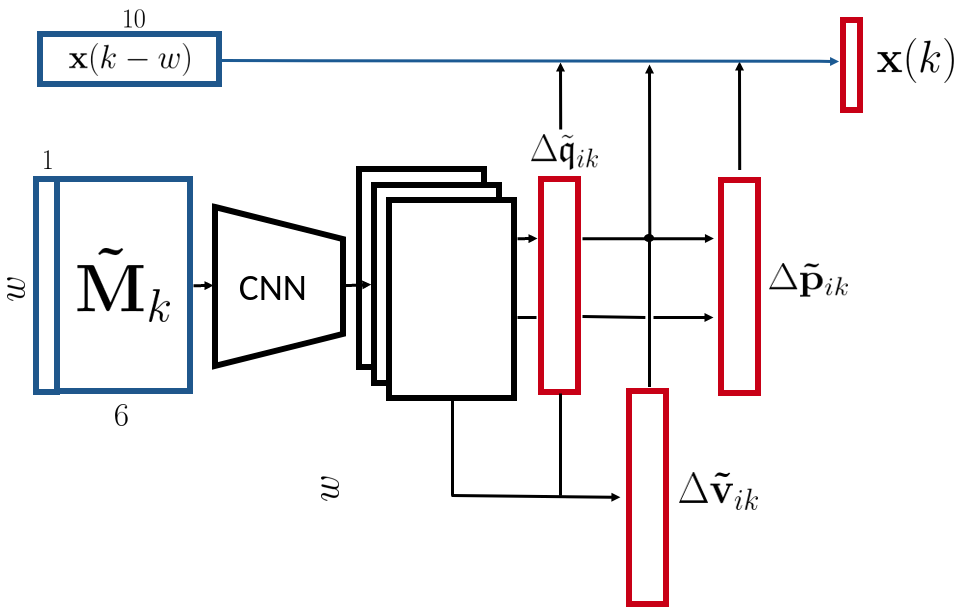
\includegraphics[width=0.75\textwidth]{img/imu_preintegration_general_net.png}
   \caption{Basic concept of the pre-integration network. Outputs in red, inputs in blue. The $\mathbf{\hat{M}}_k$ is processed by a convolutional block to generate a multidimensional feature vector.
   This vector is then used to compute the pre-integrated rotation term $\Delta\mathfrak{\tilde{q}}_{ik}$, which at its turn is used to compute the pre-integrated velocity matrix $\Delta\mathbf{\tilde{v}}_{ik}$.
   Finally, both these variables, plus the feature vector are combined to predict the final pre-integrated position $\Delta\mathbf{\tilde{p}}_{ik}$. 
   The state update is done by applying equations \ref{eq:imu_integration_2}.}
   \label{fig:basic_pre_integration_model}
\end{figure}

The main intuition behind the model is the following:
Once again, a series of convolution layers process the IMU input $\mathbf{\tilde{M}}_k$ and generate a feature vector. 
This feature vector is then used to output the first the pre-integration factor $\Delta\mathfrak{\tilde{q}}_{ik}$, corresponding to the rotation state. 
The model outputs this first, as it is the only one of the three that that can be computed on its own.
Then, both the convolutional feature vector and the pre-integrated rotation tensor are concatenated along the $w$ dimension, and used in a similar way to generate the $\Delta\mathbf{\tilde{v}}_{ik}$ term.
Finally, the feature vector and both pre-integration terms for rotation and velocity are concatenated, once again, along the $w$ dimension.
The resulting tensor is finally used by the model to generate the final pre-integration sequential term for position, $\Delta\mathbf{\tilde{p}}_{ik}$.

The current task is a challenging one, as it is supposed to mimic a very structured mathematical pipeline; the IMU double integration, but with the added twist of the pre-integrating factors.
Furthermore, one of the main aims of this final model is to be implementable real time in an hypothetical VIO platform, for which reason it is also important to keep the number of trainable parameters as low as possible.
Several iterations of fine-tuning of the model lead to the following refinements:

\textbf{Convolutional feature extractor}: For this module we leverage Temporal Convolutional Networks (TCN's) as the main building block.
This kind of CNN structure uses small dilated convolutional kernels with the same stride as the dilation rate, with the aim of rapidly expanding the receptive field of each neuron in the tensor channels \cite{DBLP:journals/corr/abs-1811-10166}.
Typically, a dilation and stride of 2 are used, so basically at layer $i$ a neuron has a receptive field of $2^i$. 

Furthermore, in order to extract both local and general features about the IMU matrix $\mathbf{\tilde{M}}_k$ we combine the TCN concept with the idea of an \emph{hourglass} structure.
This architecture was firstly introduced for the task of Human pose estimation in RGB images, achieving state-of-the-art accuracy outcomes \cite{DBLP:journals/corr/NewellYD16}.
It has proven to be efficient both at multi-scale feature extraction of spatially-correlated data and at keeping gradients alive using skip connections even with relatively deep models \cite{DBLP:journals/corr/PavlakosZDD16}.
Thanks to the extra receptive field expansion of TCN layers (which replace the traditional CNN in the hourglass), the global information can be condensed much faster, in which case we only use two recursive down-scalings of the input tensor in the hourglass module.

Something that we take extra care of, is to use reflection padding on the convolution kernels, since we don't want the information at the edges of the feature vector to be distorted by zero paddings.
Finally, the gyroscope and the accelerometer data are split and fed into to two separate hourglass modules, as it should not make any physical sense to process this data together.

\textbf{Pre-integration generator module}: the three pre-integrated variables to be generated $(\Delta\mathfrak{\tilde{q}}_{ik}, \Delta\mathbf{\tilde{v}}_{ik}, \Delta\mathbf{\tilde{p}}_{ik})$ are temporally very self-correlated. 
As such, we recycle the idea from the visual-inertial CNN-RNN architecture \cite{DBLP:journals/corr/ClarkWWMT17}, where an RNN layer (and in particular an LSTM) is exploited for this generative task (as we discussed in Section \ref{sec:VIOnet}). 
In their publication, the authors argue that using two layers of bidirectional LSTM's to generate temporally correlated data provides the best results compared to unidirectional or single-layered counterparts. 
We will not adopt any of the two ideas for different reasons:
\begin{itemize}
    \item Using bidirectional layers means that we break the very delicate alignment between the three variables in the pre-integration equations \ref{eq:pre_int_x}.
    In other words, for instance $\Delta\mathbf{\tilde{v}}_{ik}$ should only depend on $\Delta\mathfrak{\tilde{q}}_{ik'}$ for $k \in \{i, i+1, ..., i+k\}, \; k \leq w$. 
    \item Recurrent networks dramatically increase the inference time of the model, as these have to be processed sequentially.
    Since we will be needing already three recurrent layers (one for each pre-integration variable), we cannot afford stacking a second one on top.
\end{itemize}
However, we do adopt the idea of using a recurrent layer for generating these three outputs. 
In fact, empirical tests comparing GRU's \cite{DBLP:journals/corr/ChoMGBSB14} and LSTM revealed that the former outperforms both in training time and loss, so we chose it instead of LSTM.

\textbf{Pre-integrated variables: information passing}
One of the aims of this architecture and training setup is that we want to enforce the model to learn very precise temporal relationships between the variables that mimic equations \ref{eq:pre_int_x}.
As such, we implement the following constraints on $f_\theta$:
\begin{itemize}
    \item The GRU that generates $\Delta\mathfrak{\tilde{q}}_{ik'}$ will only use the TCN feature vector from the gyroscope.
    \item The output of a pre-integrated variable is passed to the next via a customly designed dense layer, that removes all connections to \emph{future} neurons. 
    E.g. $\Delta\mathfrak{\tilde{q}}_{ik'}$ can only be connected to $\Delta\mathbf{\tilde{v}}_{ik}$ for $k' \in \{i, i+1, ..., i+k\}, \; k \leq w$
    \item We don't use neither data or batch normalization between layers, as this model is very dependent on the scale of the input data.
\end{itemize}

The model with all of its refinements has a total of less than 180K trainable parameters, which is the lowest compared with the 440K of the second model, or the 18M of the first.
The overall structure is represented in Figure \ref{fig:full_pre_integration_model}, where represented by blue boxes, and outputs in red boxes.
Additionally, GRU cells are in green, untrainable connections in gray, and special, temporal aware dense connections in red.

\begin{figure}[h]
   \centering
   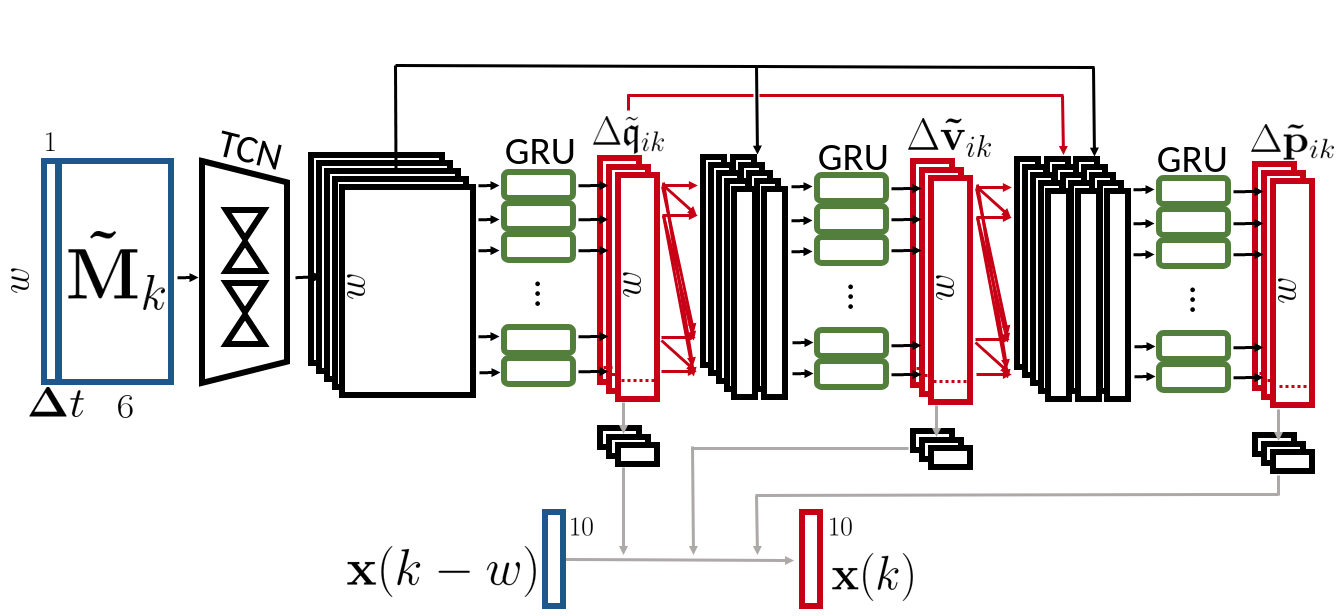
\includegraphics[width=0.95\textwidth]{thesis_template/img/pre_integration_full.png}
   \caption{Refined pre-integration network. Outputs in red, inputs in blue. Customized connections as red lines. Non-trainable connections as gray lines.
   The convolutional block is substituted by a recursive hourglass convolutional architecture with TCN layers.
   The layers that generate the pre-integrated variables are GRU units, and the custom connections ensure that variables can only depend on samples from the past and not the future, along the $w$ dimension.}
   \label{fig:full_pre_integration_model}
\end{figure}

In Chapter \ref{chap:experiments}, we will discuss our different attempts at training this model.
\chapter{Experiments}\label{chap:experiments}

In this chapter, we will be providing more graphic material for the different models detailed in chapter \ref{chap:methods}.
We will be going over the three models and their experiments again, providing extra results that were not shown earlier.

\section{First model: CNN speed regressor}\label{sec:speed_regression_model}

This model is a deep CNN that predicts the average velocity norm (i.e. speed) of a unit from a window of IMU measurements. 
We test this model on the inertial data of the EuRoC dataset, which we found is extremely corrupted by vibration noise, making the learning task much difficult. 
We remove the noise using the filtering technique specified in the Appendix section \ref{sec:euroc_filtering}, and after 150 epochs we manage to fit in the training set.
Furthermore, we do some normalization preprocessing of the IMU input data, which we also found was necessary to fit the model.
Without these two requirements, the architecture was not able to make sense of the data.

Figure \ref{fig:speed_prediction_filtered_vs_unfiltered} shows the results of our predictions on the training set. 
On the left plot, noise has been removed from the dataset using the low-pass filtering. 
Notice how the predictions on the left image (unfiltered data) during the first 5000 samples are as nearly as accurate as in the filtered counterpart.
This is because during the first seconds of the flight, the drone is moved by hand, and therefore there is no vibration noise.
We can however see that, in the presence of high frequency noise, the predictions are much less accurate.

\begin{figure}[h]
   \centering
   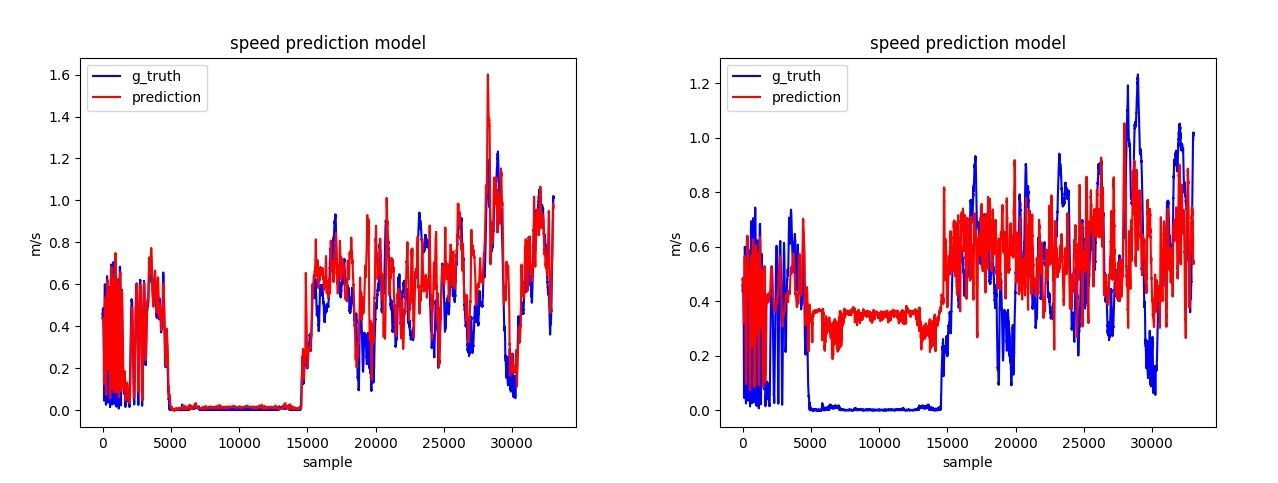
\includegraphics[width=0.95\textwidth]{thesis_template/img/speed_prediction_filtered_vs_unfiltered.jpeg}
   \caption{Linear speed regression in the EuRoC training set, with (left) and without (right) the dataset pre-processing specified in appendix Section \ref{sec:euroc_filtering}.
   The regressor is not able to fit the training data when the IMU noise is not filtered out.}
   \label{fig:speed_prediction_filtered_vs_unfiltered}
\end{figure}

Furthermore, Figure \ref{fig:speed_prediction_filtered_vs_unfiltered_validation} shows the same experiment than Figure \ref{fig:speed_prediction_filtered_vs_unfiltered} but evaluated on a separate held-out test set not used during training.
In this case, the model cannot properly predict any of the two datasets, but on top of that the predictions oscillate more in the unfiltered case.

\begin{figure}[h]
   \centering
   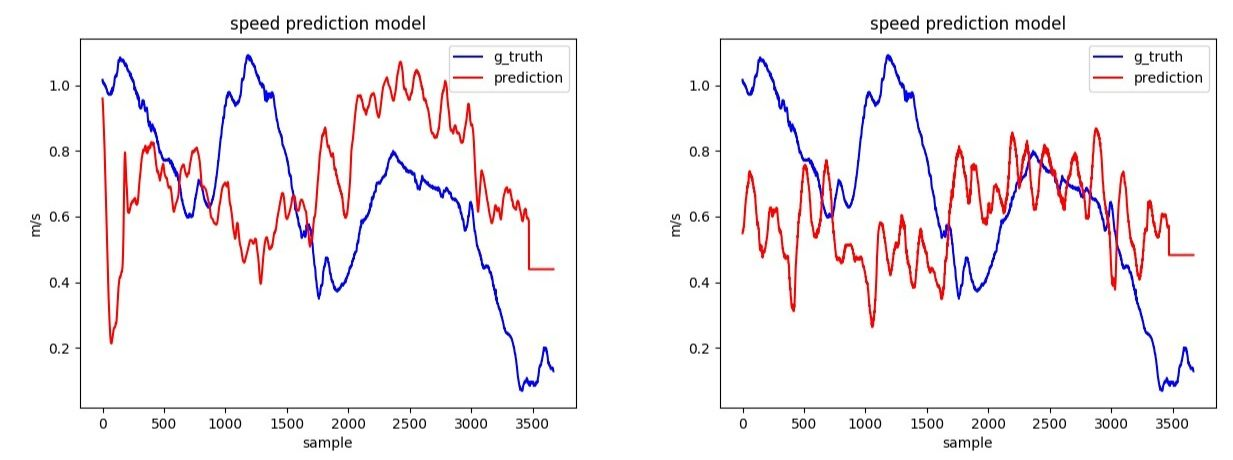
\includegraphics[width=0.95\textwidth]{thesis_template/img/speed_prediction_validation_filtered_vs_unfiltered.jpeg}
   \caption{Linear speed regression in the EuRoC held-out validation set, with (left) and without (right) the dataset pre-processing specified in appendix Section \ref{sec:euroc_filtering}.
   The regressor is not able to properly predict the correct speed values from the ground truth, but the predictions are even less accurate without the filtering.}
   \label{fig:speed_prediction_filtered_vs_unfiltered_validation}
\end{figure}

To evaluate the efficacy of our filtering strategy, we apply it to an ideal EuRoC dataset, generated with a Visual-Inertial simulator from Zurich eye. 
This dataset is completely free of IMU noise, and has been generated from the flight sequence "Machine Hall 1", which was not used to train our model, so we consider it as a valid test set.
We use once again our model to regress the linear speed across time (see Figure \ref{fig:speed_prediction_filtered_vs_unfiltered_ideal}).
The predictions of the model are not very accurate, but it appears like the model has indeed learned something about how to estimate the speed of the drone.
We also perform a sanity check by predicting on an unfiltered version of this ideal dataset, and verify that the predictions very similar than with the filtered data (right plot).
This means that, as we hypothesize in Section \ref{sec:euroc_filtering}, the low frequencies (smaller than 10Hz) contain nearly all the relevant information for the state estimation task, and the higher ones can be removed quite safely.

\begin{figure}[h]
   \centering
   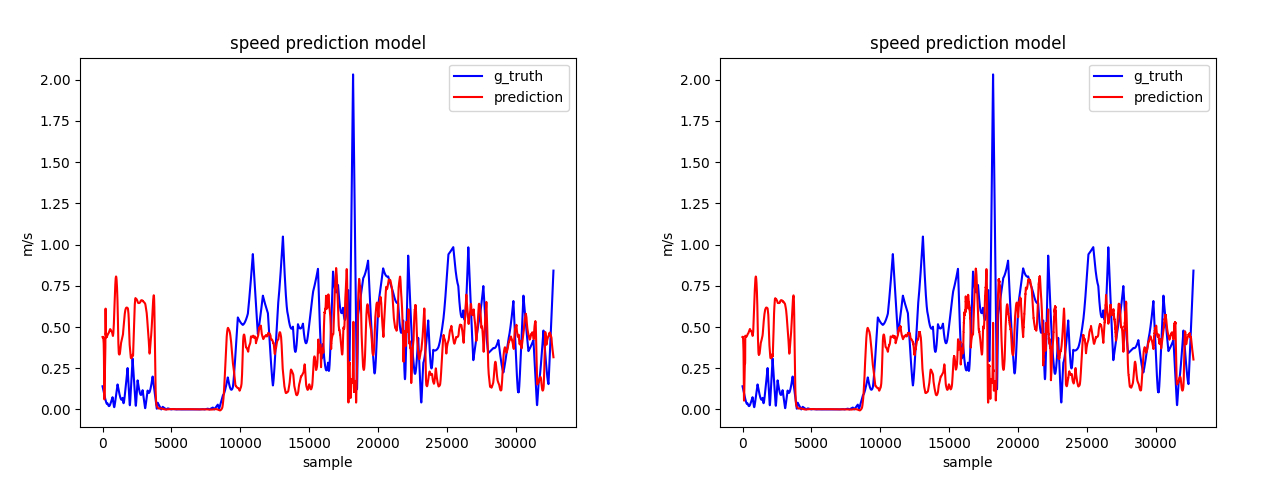
\includegraphics[width=0.95\textwidth]{thesis_template/img/speed_prediction_ideal_filtered_vs_unfiltered.jpg}
   \caption{
   Linear speed regression in an ideal, noiseless, EuRoC test set, with (left) and without (right) the dataset pre-processing specified in appendix Section \ref{sec:euroc_filtering}.
   Both predictions look almost identical, which confirms that the low-frequency components of the IMU signal contain the most relevant information needed by the model to regress the speed norm value.}
   \label{fig:speed_prediction_filtered_vs_unfiltered_ideal}
\end{figure}

\section{Second model: IMU state integrator}

This second model aims at reproducing IMU integration with a deep model. 
Of course, one important requirement is that the model should learn how the noise and bias of the inertial sensor work, so that it can remove them intrinsically as much as possible.
We do this by using as training set the noiseless ground truth data as target.
To evaluate the performance of the trained models for this task, we design two different experiments that evaluate their short-term and long-term reliability. 

The first experiment, which we call the \emph{one-step} experiment, inputs to the models a starting state $\mathbf{x}(k-w)\in\mathbb{R}^{10}$ together with $w$ IMU measurements from sample $k-w$ until $k$: $\mathbf{\hat{M}}_k\in\mathbb{R}^{w\times6}$ and expects to receive the output state $\mathbf{\hat{x}}(k)$, which is compared with the corresponding ground truth measurement $\mathbf{x}(k)$.
This experiment is used safety check, as normally the system state estimate is not expected to drift significantly because of noise in just $w$ samples.

Once the model passes the first experiment, the second one is performed, which we call the \emph{iterative} experiment.
In this case, an initial state $\mathbf{x}(0)$ is given to the system, together with a succession of n windows of IMU measurements: $\left(\mathbf{\hat{M}}_w,\mathbf{\hat{M}}_{2w},...,\mathbf{\hat{M}}_{nw}\right)$, with overlap in just the last sample (i.e. overlap 1). 
The system must use all the inputs to generate a sequence of predictions $\left(\mathbf{\hat{x}}_w, ..., \mathbf{\hat{x}}_{nw}\right)$, using the intermediate predictions its own state input for next iteration.

\subsection{First model iteration: $\mathbf{x}(k),\; \mathbf{\hat{x}}(k)\in\mathbb{R}^{10}$}
For the first iteration of this model, we train the architecture described in Figure \ref{fig:state_int_v0}, where the output state is a 10-dimensional vector containing the predicted position, velocity and rotation, in unit quaternion form. 
As a proof of concept, we train this model on a rather flat flight from the BB dataset (\emph{Thrice}), and with a maximum speed of 2m/s, which is also quite slow. 

We then test the model on a second flight sequence (\emph{bentDice}, $v_{max}=2m/s$), which is actually rich in 3D motion.
We perform first the one-set integration test against this test set. 
As we showed in Figure \ref{fig:imu_int_50} in last section, the model is quite reasonably able to predict the position x and y, and the speed of the drone also in these two axes. 
However, it fails to properly calculate the rotation, or the z component of $\mathbf{p}$ and $\mathbf{v}$. 
Figure \ref{fig:imu_int_50_r10_3d} provides a 3D visualization of the position vector, where we can see that the predicted positions are not particularly better than IMU integration for most of the trajectory.

\begin{figure}[h]
   \centering
   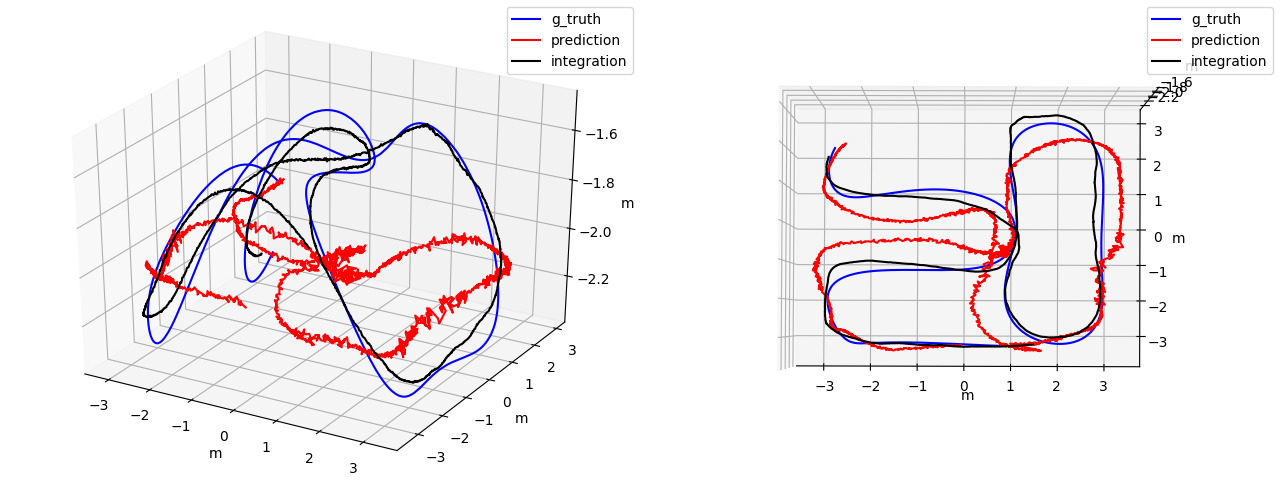
\includegraphics[width=0.85\textwidth]{thesis_template/img/imu_int_50_3d.jpg}
   \caption{3D visualization of the position ground truth, compared with the model predictions and IMU double integration algorithm. 
   3D view (left) vs top view (right). The model under-performs double-integration in all three dimensions, especially in the z axis, because the training data was planar and the model could not learn motion in this dimension.}
   \label{fig:imu_int_50_r10_3d}
\end{figure}

\subsection{Second model iteration: $\mathbf{x}(k)\in\mathbb{R}^{10},\; \mathbf{\hat{x}}(k)\in\mathbb{R}^{9}$}\label{sec:exp_imu_int_so3}

While z-dimension problem in the previous approach is expected, since the original training set of the model was a quite flat flight, we hypothesize that the rotation problem is due to the high non-linearity of the quaternion loss term (described in \ref{eq:q_state_loss}).
To fix this, we change the output format of the model, so that the predicted rotation component is in Lie algebra, which allows to use MSE loss \ref{eq:state_so3_loss} instead of the highly nonlinear quaternion angle loss.
An exponential mapping can then be applied to remap this rotation component back to quaternion form.

This new approach is retrained, this time on the 3D \emph{bentDice} dataset, also with a maximum speed of 2m/s.
Then, the one-step integration experiment is repeated on a split test set of the same flight sequence, which yields the results in Figure \ref{fig:imu_so3_bentdice_val}, where it is evident that the fit of the $\boldsymbol{\mathfrak{q}}$ rotation vector is much better than in Figure \ref{fig:imu_int_50}.

\begin{figure}[h]
   \centering
   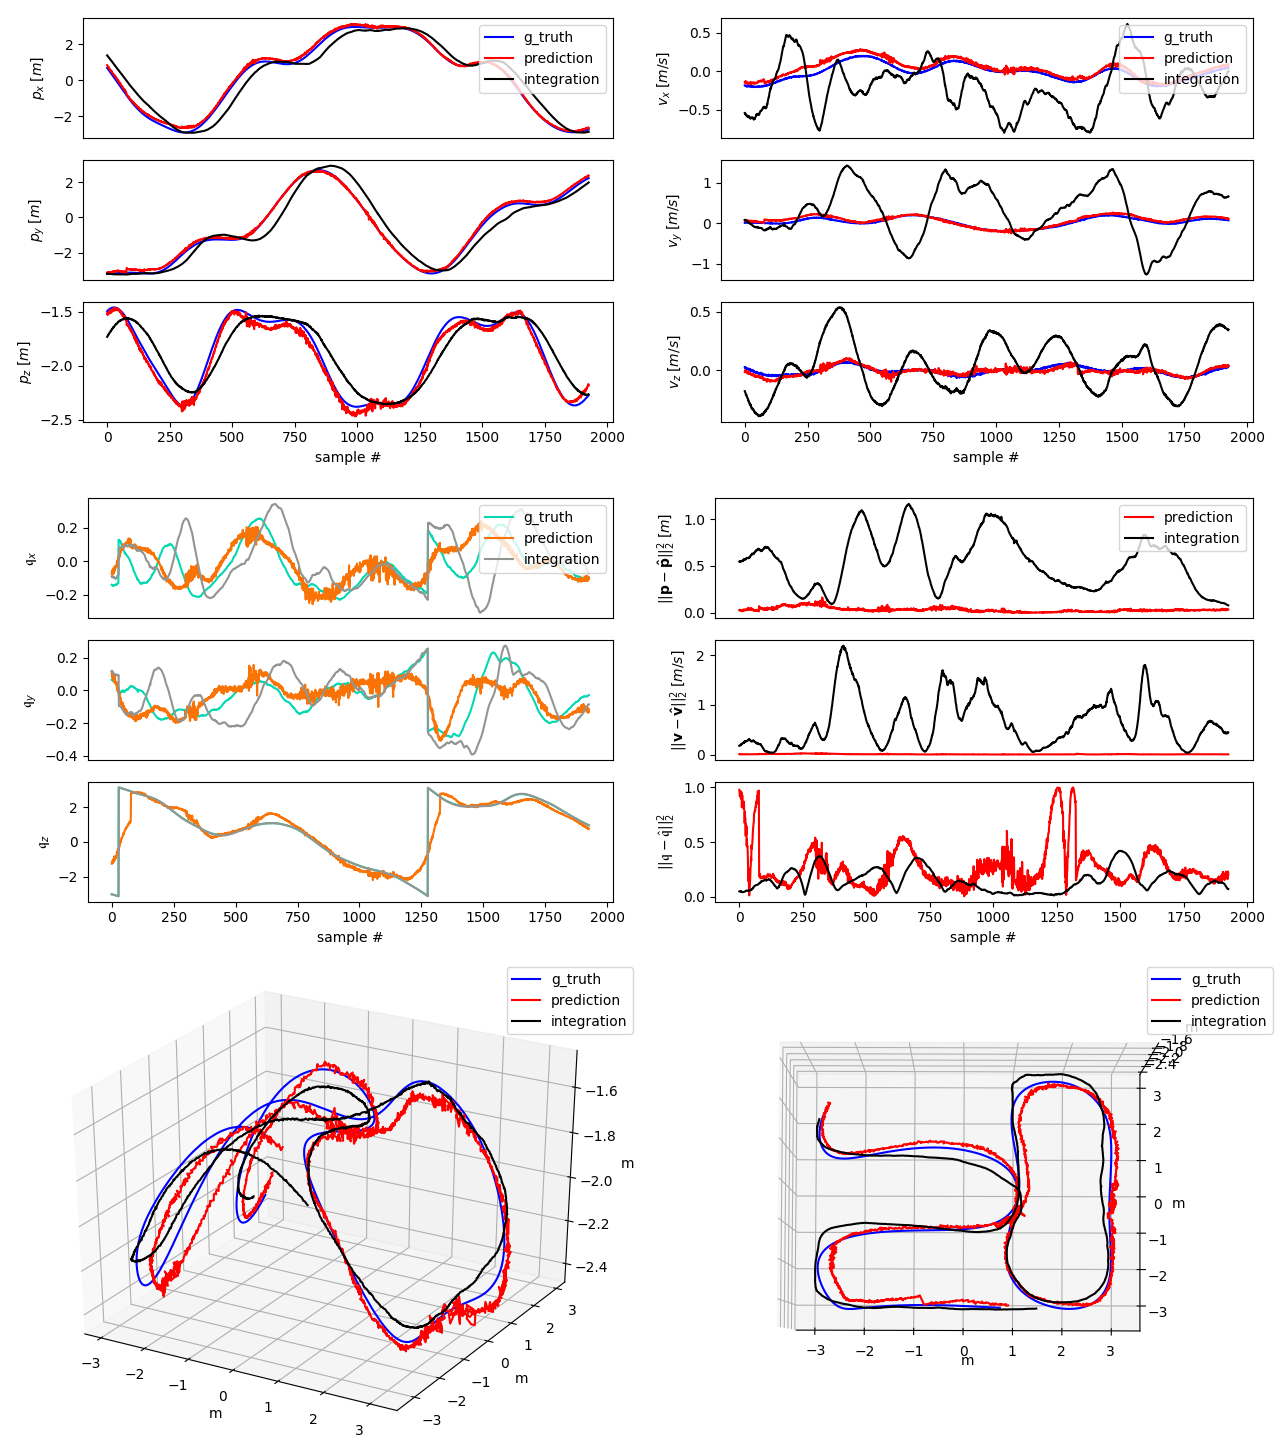
\includegraphics[width=0.85\textwidth]{thesis_template/img/imu_int_50_so3_bentDice_validation_full.jpg}
   \caption{Results of the $\mathfrak{so}(3)$ based model on a split test set from the \emph{bentDice} sequence compared with ground truth and IMU double integration. From left to right, and top to bottom, the plots represent: $\mathbf{p}$, $\mathbf{v}$, $\boldsymbol{\mathfrak{q}}$, the errors wrt. the ground truth, and the 3D views of $\mathbf{p}$.}
   \label{fig:imu_so3_bentdice_val}
\end{figure}

We proceed to repeat the same experiment with a segment of a more complex flight (\emph{tiltedThrice}), and also more aggressive, with top velocities of 6m/s. 
Furthermore, none of the fragments of this sequence have not been used at all during training time.
A similar comparative figure for this experiment is provided in Figure \ref{fig:imu_so3_tiltedThrice_val}. 
We verify that, for this set, the model quite accurately predicts the x and y positions and velocity vector, but has a bit of trouble sorting out the rotation (mainly due to the high amount of sign flips) and the z position. 

\begin{figure}[h]
   \centering
   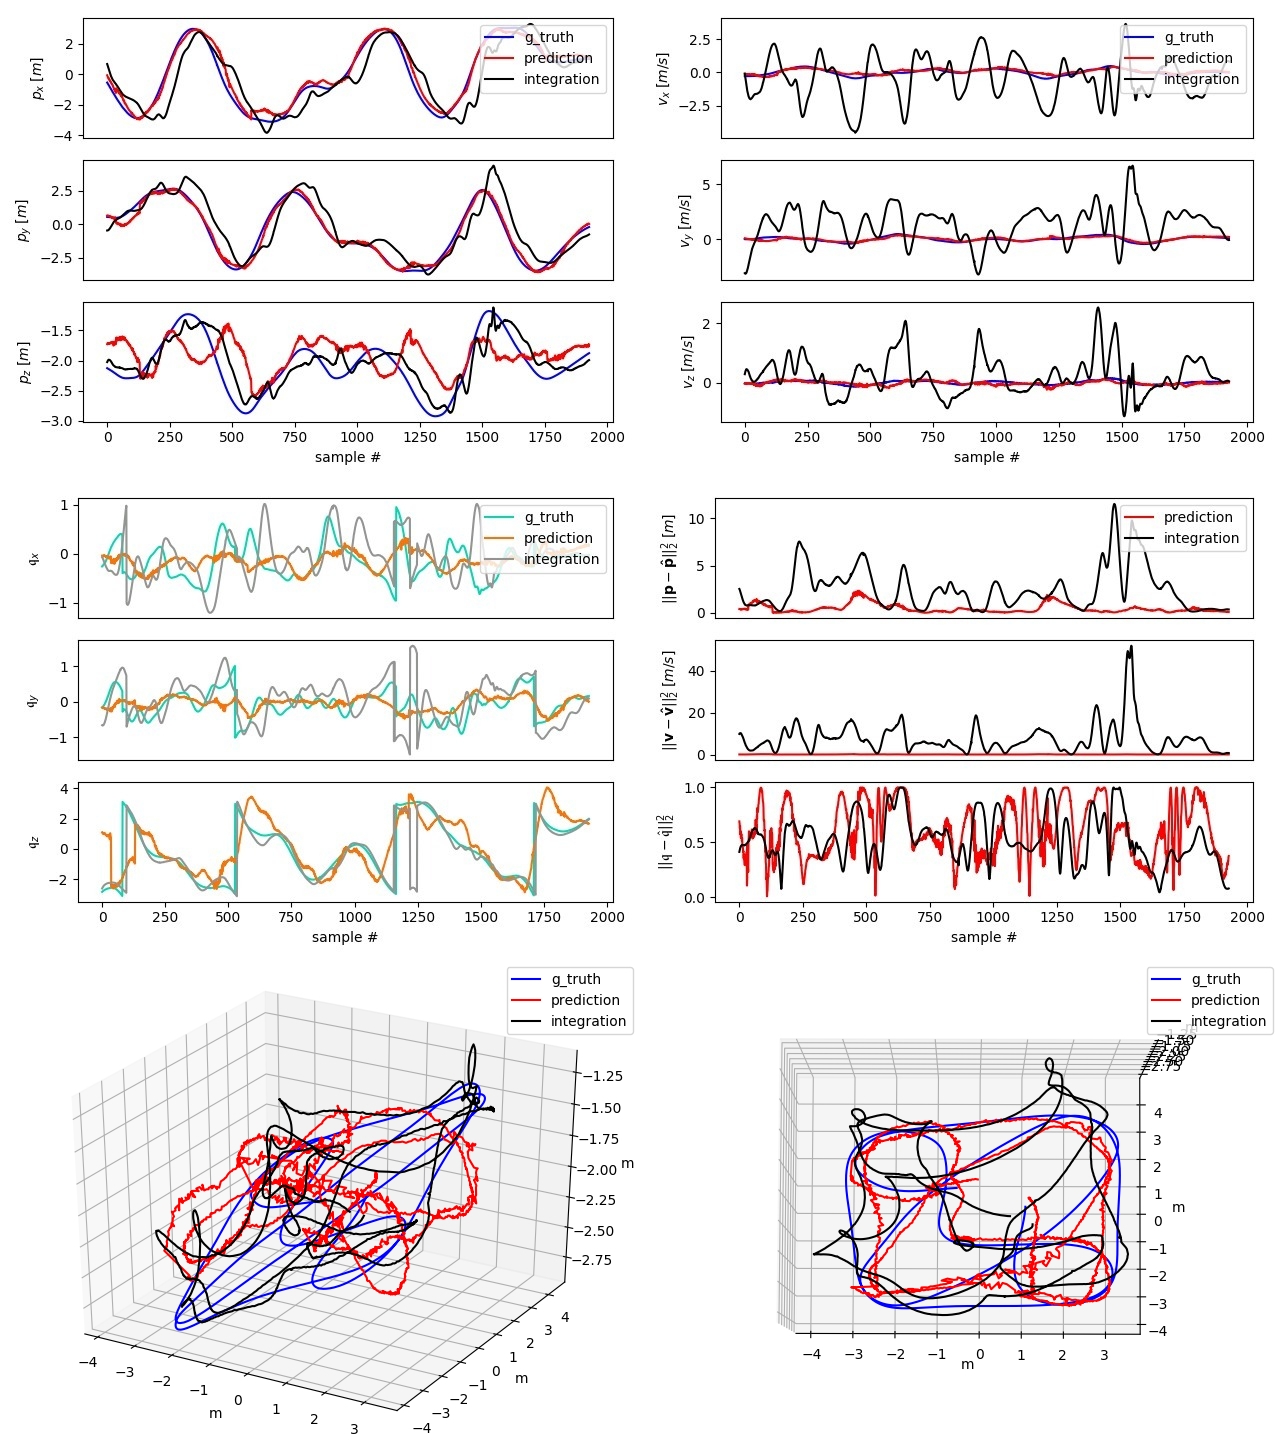
\includegraphics[width=0.85\textwidth]{thesis_template/img/tilted_thrice_so3_full.jpg}
   \caption{Results of the $\mathfrak{so}(3)$-based IMU integration deep model on a fragment of the test sequence \emph{tiltedThrice}@6m/s compared with ground truth and IMU double integration. From left to right, and top to bottom, the plots represent: $\mathbf{p}$, $\mathbf{v}$, $\boldsymbol{\mathfrak{q}}$, the errors wrt. the ground truth, and the 3D views of $\mathbf{p}$.}
   \label{fig:imu_so3_tiltedThrice_val}
\end{figure}

As a sanity check, we perform the \emph{iterative experiment} using both the training set (i.e. with the \emph{bentDice} training sequence), and the \emph{tiltedThrice} test set. 
The aim of this experiment is to see if the model can overcome somehow the noise of the IMU at a longer time span.
In Figure \ref{fig:imu_so3_iterative_bentDice_vs_tiltedThrice_pos} we show the results for the position estimate for both datasets.
We don't show the results for the IMU double integration because they drift significantly more, and they completely distort the view of the plots. 

\begin{figure}[h]
   \centering
   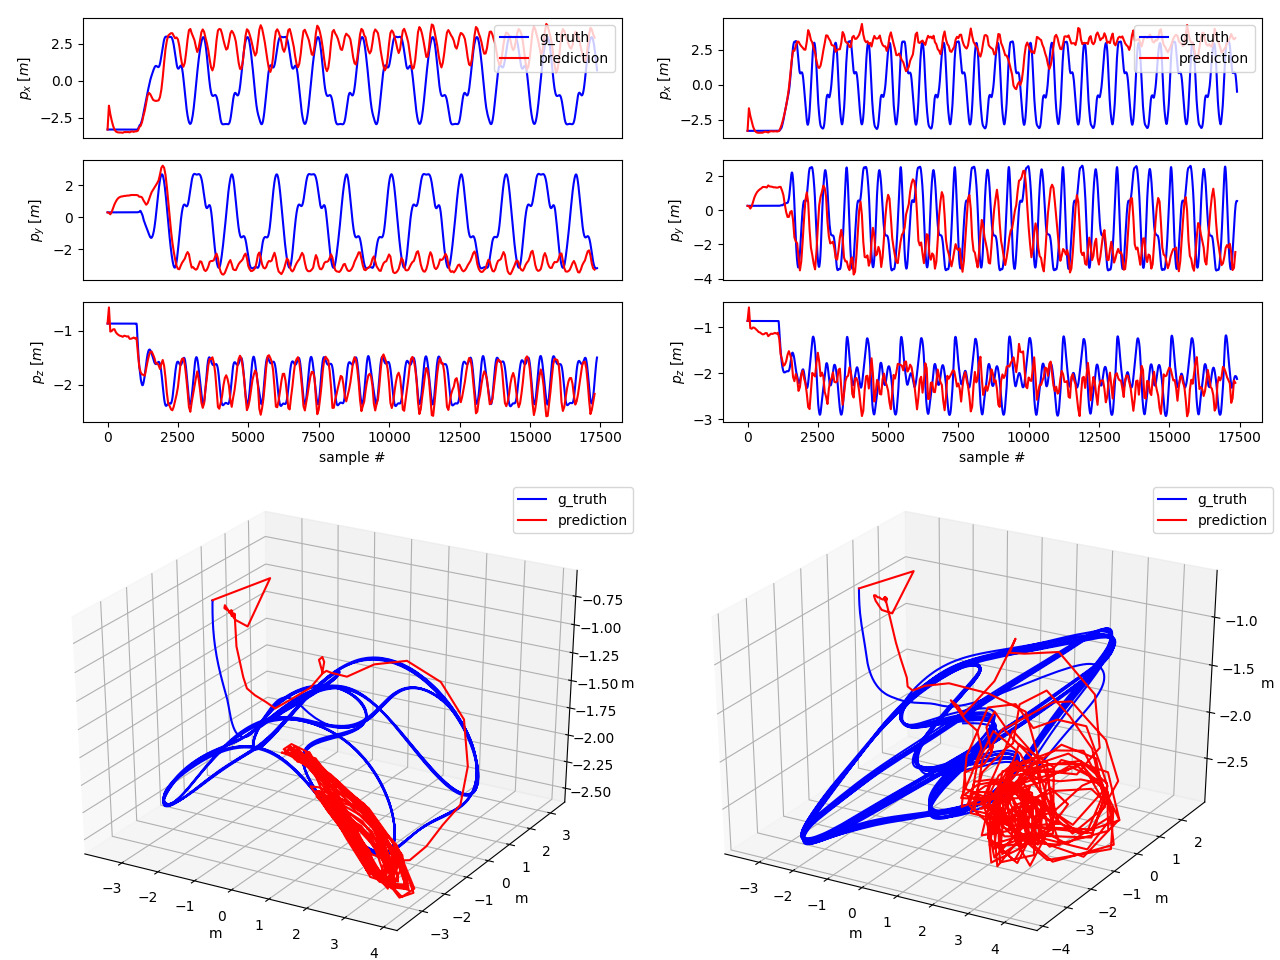
\includegraphics[width=0.85\textwidth]{thesis_template/img/iterative_bentDice_vs_tiltedThrice.jpg}
   \caption{Results of the iterative experiment on both the training set (left column) and test set (right column), using the \emph{bentDice}@2m/s and \emph{tiltedThrice}@6m/s respectively. It can be shown that the model cannot properly follow the trajectory in neither of the cases, although it does not drift to arbitrarily large values.}
   \label{fig:imu_so3_iterative_bentDice_vs_tiltedThrice_pos}
\end{figure}

From Figure \ref{fig:imu_so3_iterative_bentDice_vs_tiltedThrice_pos}, we can see that the model is not quite following the trajectory, and is instead doing some sort of periodic movements for the three output $(\mathbf{\hat{p}}, \mathbf{\hat{v}}, \mathfrak{\hat{q}})^T$. 
This leads to the hypothesis that the model is not really learning proper integration, but some kind of fixed mapping between initial state and final state.
At the end of the day, it is probably the easiest thing to do for a deep model, since both states are quite similar when using a window of $w=50$, which only corresponds to a time uncertainty of 0.5 seconds in the BB dataset. 

To test this hypothesis, and to verify if the architecture of the model makes sense at all, we run the iterative experiment again for the \emph{bentDice} training dataset with four variants. For each of these, we deactivate some connections of the network architecture from Figure \ref{fig:state_int_v0}, and perform inference on the specified dataset. The results of the following four tests are shown in Figure \ref{fig:iterative_bentDice_contributions}:
\begin{enumerate}
    \item\label{item:iterative_no_CNN} In the upper-left plot, we remove the connections from the CNN module in the concatenating layer.
    \item\label{item:iterative_no_IMU_skip} In the upper-right plot, we remove the skip connections from the IMU matrix in the concatenating layer.
    \item\label{item:iterative_just_state_0} In the lower-left plot, we remove all connections except for the initial state.
    \item\label{item:iterative_just_imu_data} In the lower-right plot, we remove the connections of the initial state.
\end{enumerate}

\begin{figure}[h]
   \centering
   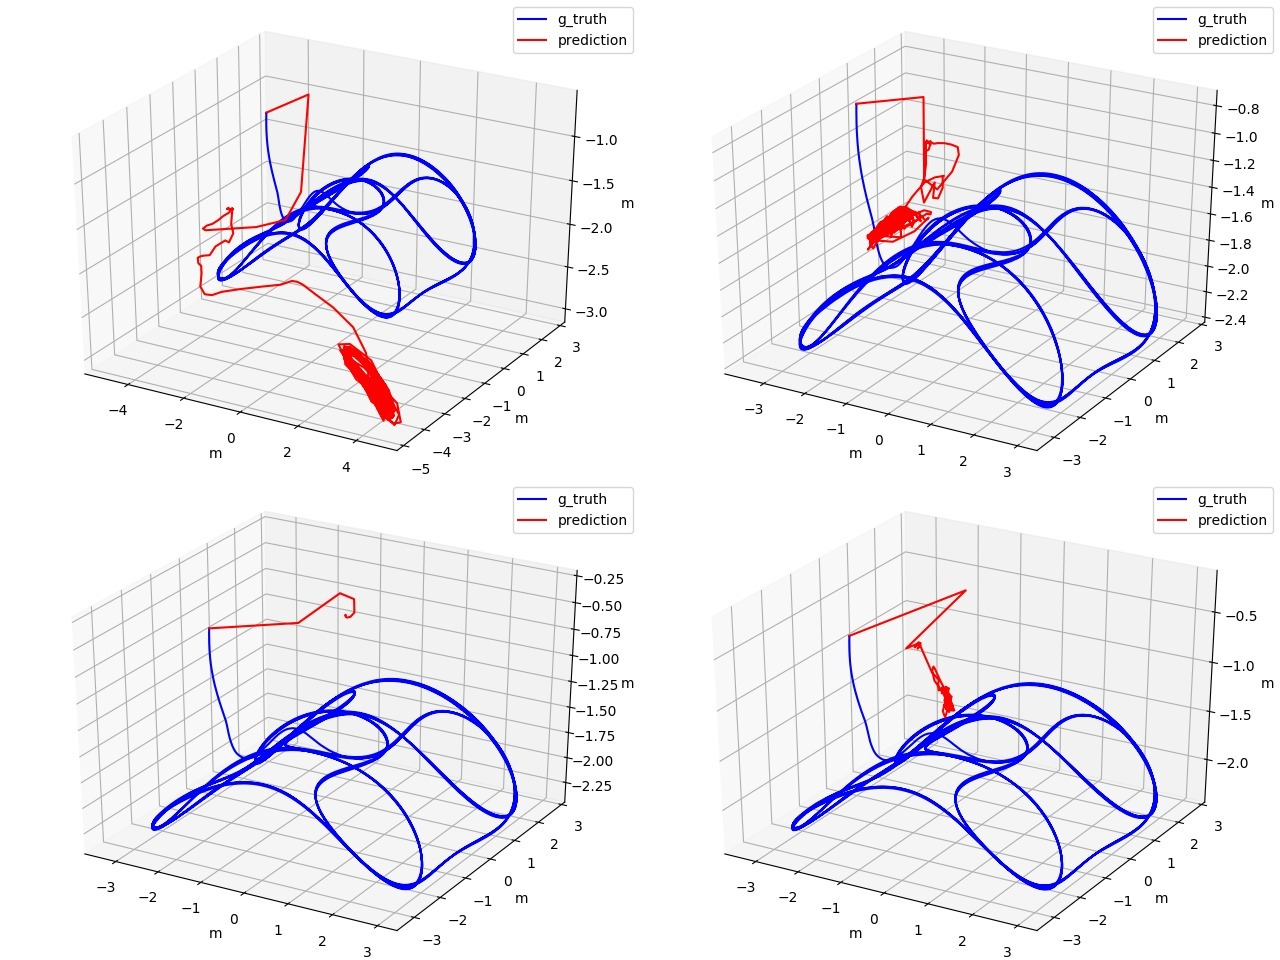
\includegraphics[width=0.85\textwidth]{thesis_template/img/iterative_bentDice_contributions.jpg}
   \caption{Results of the iterative experiment on the training set (\emph{bentDice}@2m/s), where several connections have been disabled in the network. Upper-left: no CNN information. Upper-right: no IMU information. Lower-left: Only initial state information. Lower-right: no initial state information.}
   \label{fig:iterative_bentDice_contributions}
\end{figure}

After accurate analysis of the results shown in Figure \ref{fig:iterative_bentDice_contributions}, we can see that the model is actually learning some sort of IMU integration, in fact. 
In experiment (\ref{item:iterative_just_state_0}.), where only the initial state is being used, we see that there is barely any motion at all
This is what one would expected of IMU integration, because the system should use the IMU data to deduce how the initial state has changed. 
However, for this experiment the IMU data contribution has been completely shortcut, and therefore the state should not be changing. 

On the other hand, in experiment (\ref{item:iterative_just_imu_data}.), which does not have information about the initial state, we can see that in fact there is a lot of small movements around position $(0, 0, -1)^T$.
If the deep model has correctly learned to integrate the IMU data, but has no information about the initial state, then one would indeed expect to see small movements around point $(0, 0, 0)^T$. We can therefore see that the model is actually learning correctly integration in the x and y axes, but it is somehow overfitting the z axis.

Finally, by comparing experiments (\ref{item:iterative_no_CNN}.) and (\ref{item:iterative_no_IMU_skip}.), we can see that most of the unwanted periodic motion comes in fact from the skip connection of the IMU matrix, which probably is distracting the model from learning. 
This means that indeed the convolutional layers may be useful to process the IMU, and extract relevant features for integration. 

\section{Third model: IMU pre-integrator}

The last training approach that we study is what we call the IMU \emph{pre-integrator} (derived in Section \ref{sec:pre_int_training}).
This model is in fact two concatenated models, where only the former is trainable.
It receives as input just the IMU data $\mathbf{\hat{M}}$, from which it is supposed to predict the pre-integration states $(\Delta\mathfrak{\tilde{q}}_{ik}, \Delta\mathbf{\tilde{v}}_{ik}, \Delta\mathbf{\tilde{p}}_{ik})$ derived in \ref{sec:pre_int_training} for all samples $k$ in the time window $[i, i+w]$.
With these pre-integration variables, then the latter model can calculate a prediction for the new state $\mathbf{x}(i+w)$ given $\mathbf{x}(i)$ in a fixed, non-trainable way.

This task proved to be difficult to train for four different reasons.
\begin{itemize}
    \item The number of trainable parameters is quite small (less than 180K).
    \item The output space is large, and larger than the input space. In particular, the model outputs three matrices of dimensions $w\times3$, plus one vector of size $10$. 
    When using $w=50$, this represents a total of $460$ output values, while the input is $300$-dimensional.
    \item There are non-trivial relationships between all the variables in the output space.
    \item The input data cannot be normalized because the scale is important in this problem.
\end{itemize}
Therefore, to be able to properly solve this prediction task, the model is forced to exploit as much as possible the temporal dependence between the variables of the output space by means of a very guided architecture.
Inspired from the literature, we train the model with four different losses: 3 for the pre-integration terms, and one for the state output. 
We derived in Section \ref{sec:pre_int_training}, however, how we can use the fixed nature of the second model to reduce these four losses back to three. 

The model is again trained using the \emph{bentDice} sequence from the Blackbird dataset at a maximum speed of 2m/s, and using an hyperparameter value for the window length of $w=50$.
Following the indications in \cite{DBLP:journals/corr/ClarkWWMT17}, we choose the parameters $a=1$, and $b=0.1$ for our loss function for the first 30 epochs. 
Then, for 20 more epochs, increase $b$ to $0.5$. 
The \emph{one-step} experiment is first performed on a held out part of the \emph{bentDice} flight, and on the harder \emph{tiltedThrice} flight, as with the previous model.
For now, we concentrate on the first three outputs of the model, i.e., the pre-integrated values $(\Delta\mathfrak{\tilde{q}}_{ik}, \Delta\mathbf{\tilde{v}}_{ik}, \Delta\mathbf{\tilde{p}}_{ik})$. The results of this experiment are provided in Figure \ref{fig:pre_integration_original_4loss_bentDice_vs_tiltedThrice}.

\begin{figure}[h]
   \centering
   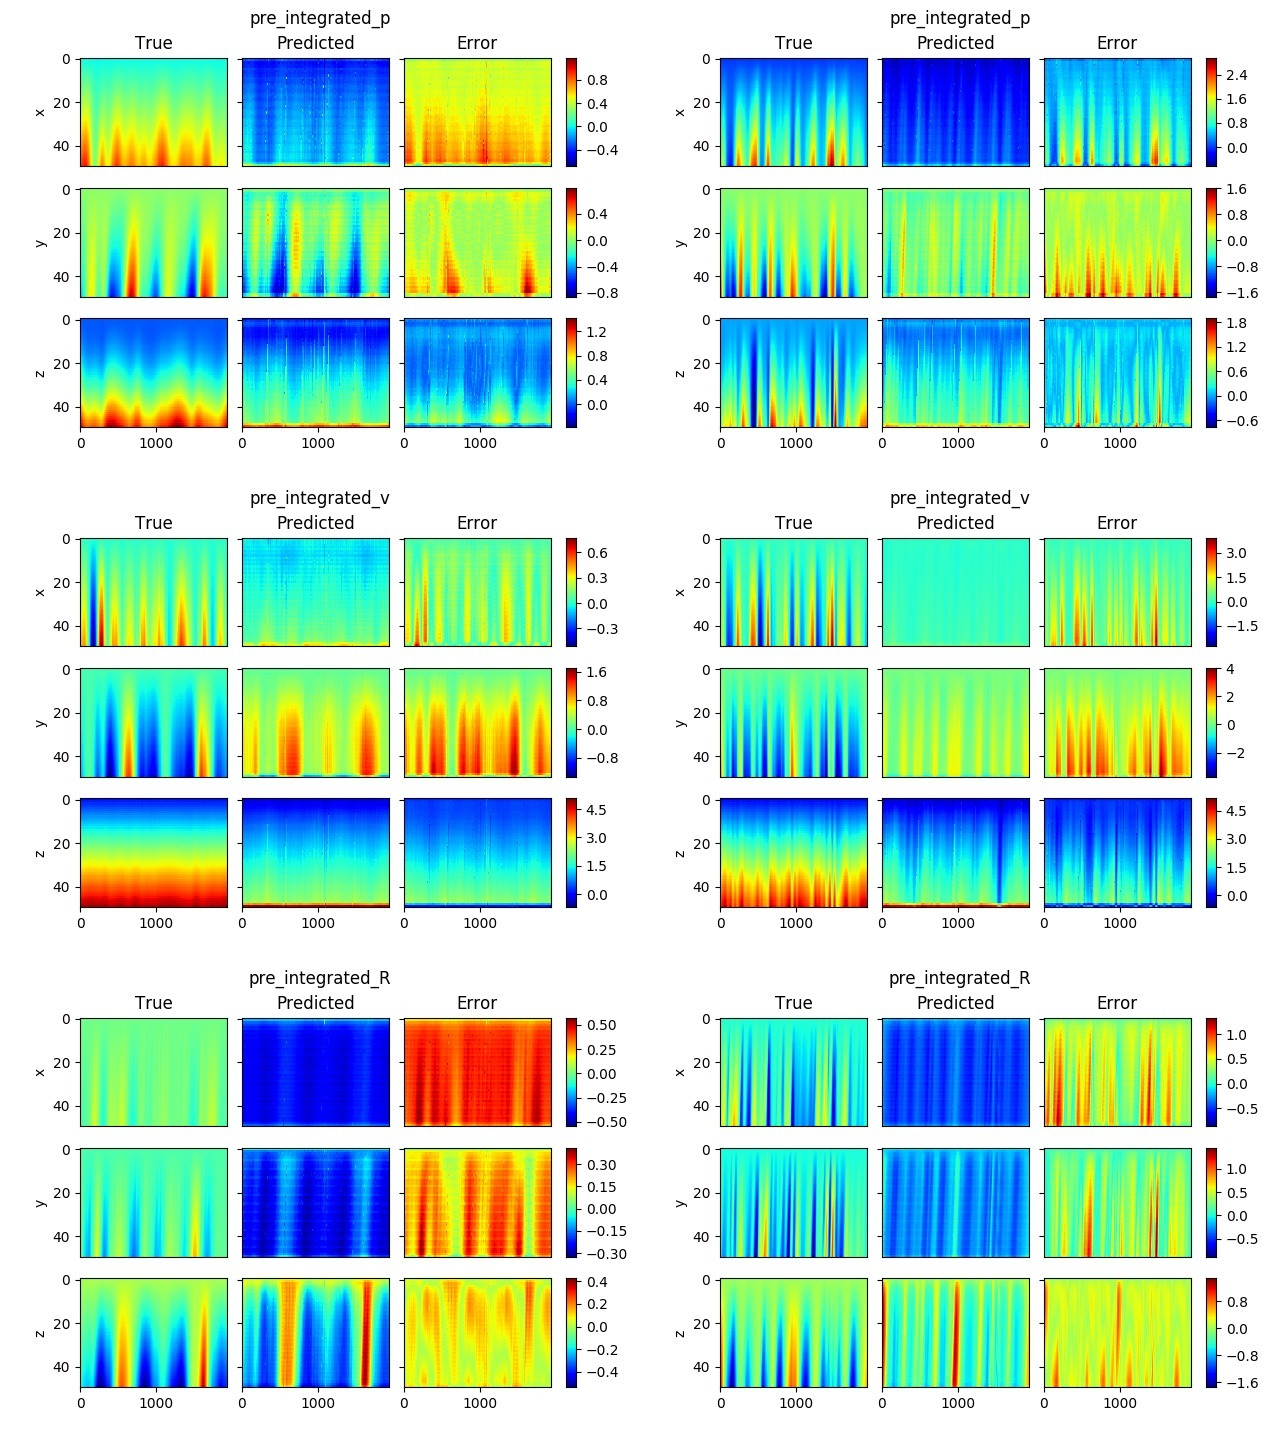
\includegraphics[width=0.85\textwidth]{thesis_template/img/original_4_loss_bentDice_vs_tiltedThrice.jpg}
   \caption{Pre-integration results of the one-step experiment on the validation sets \emph{bentDice}@2m/s (1st column) and \emph{tiltedThrice}@6m/s (2nd column). From top to bottom, rows represent $\Delta\mathbf{\tilde{p}}_{ik}, \Delta\mathbf{\tilde{v}}_{ik}$ and $ \Delta\mathfrak{\tilde{q}}_{ik}$. Inside of each of the 6 plots, the three rows are the x, y, and z components of the specific variable.}
   \label{fig:pre_integration_original_4loss_bentDice_vs_tiltedThrice}
\end{figure}

From Figure \ref{fig:pre_integration_original_4loss_bentDice_vs_tiltedThrice} it is important to understand what each axis in each subplot means.
The horizontal axis still represents the time domain; each column is the output of the model for time sample $k$.
In this case, the input is the window of IMU measurements $\mathbf{\hat{M}}_k$, from $k-w$ until $k$.
Since the pre-integrated variables (model outputs) are $\mathbb{R}^{w\times 3}$ matrices, where the $3$ corresponds to the $(x, y, z)$ components, each output is decomposed into three subplots, where each one has $w$ outputs, sorted as columns.

We can therefore see in Figure \ref{fig:pre_integration_original_4loss_bentDice_vs_tiltedThrice} that indeed the model has a much less error in the last row, which corresponds to the value that is used to compute the output state, and thus receives the 4th loss component.
Although it is important that the model has a low error on this term, the pre-integrated values should be \emph{smooth} vertically.
This sharp discontinuity means that the model has not quite learned the task well. 
Furthermore, we can see that in some cases the predictions do not quite match the ground truth.
We empirically found that a very good way to visually condense all the metrics of the model into a single plot, is to let the model reconstruct the 3D position trajectory.
Since the $\mathbf{\hat{p}}$ value depends on all the variables in the output space, it has a lot of information regarding the general performance. 
The two reconstructed trajectories are shown in Figure \ref{fig:position_3D_original_4loss_bentDice_vs_tiltedThrice}, where it can be seen that the model has trouble especially with the $z$ component of the integration.

\begin{figure}[h]
   \centering
   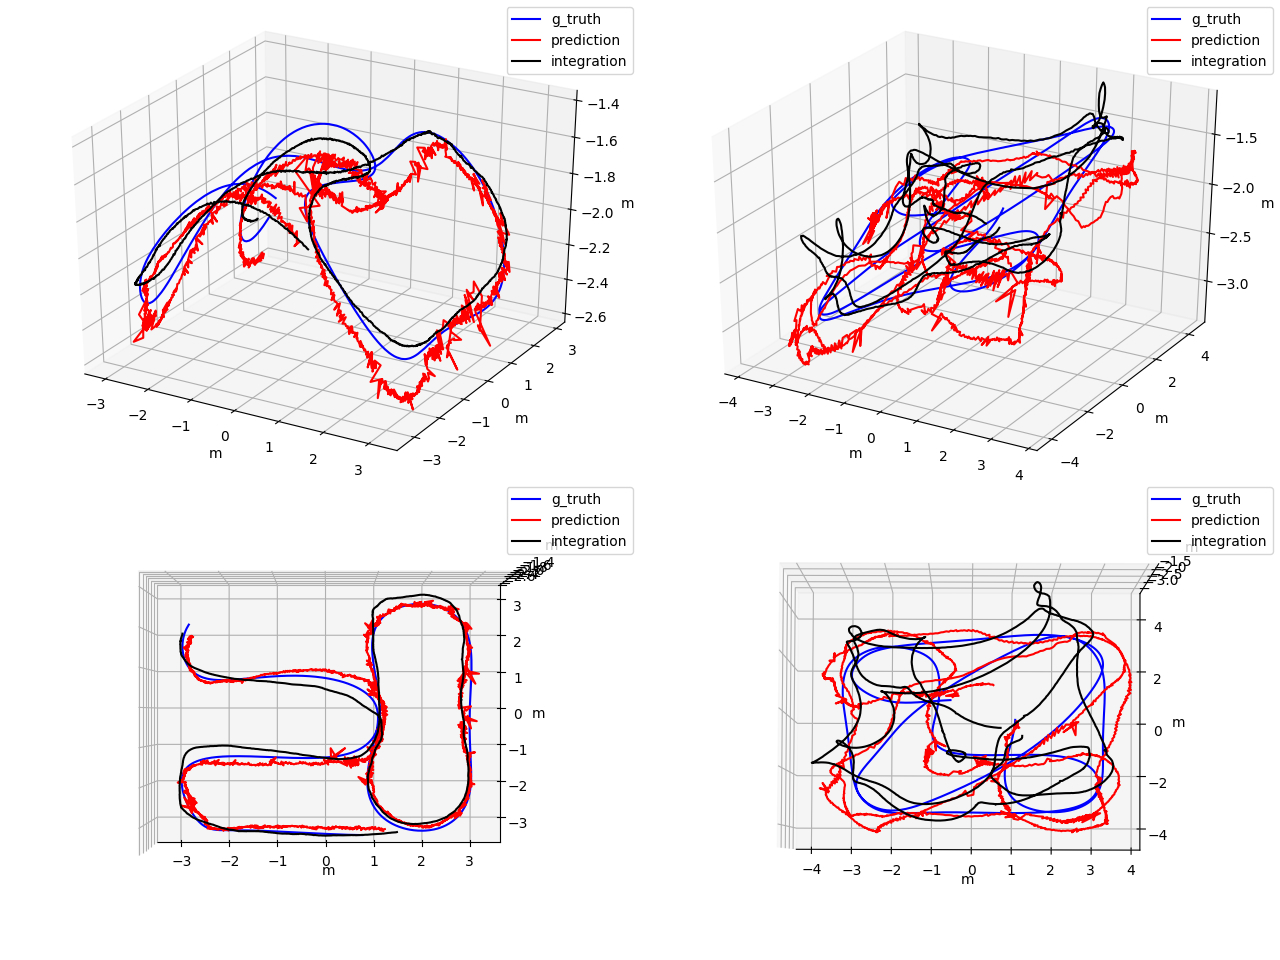
\includegraphics[width=0.85\textwidth]{thesis_template/img/pre_integration_original_4_loss_bentDice_vs_tiltedThrice_3D.jpg}
   \caption{Position vector output of the one-step experiment on the validation sets \emph{bentDice}@2m/s (1st. column) and \emph{tiltedThrice}@6m/s (2nd column).
   The precision of the algorithm in the x and y axes is much higher than in the z axis.}
   \label{fig:position_3D_original_4loss_bentDice_vs_tiltedThrice}
\end{figure}

In an attempt to fix the \emph{smoothness} problem, we introduce two added regularization terms to the training graph.
The first, harshly penalizes if the first row of any pre-integrated value differs from zero.
The second, adds a loss term proportional to the differences between two successive rows in the output, in a sort of way acting as a \emph{diffusion} mechanism along the time ($w$) dimension.
In other words, this latter regularization term penalizes sharp discontinuities in the pre-integrated values, with the aim of enforcing a temporal consistency in the output.
This regularization is weighted by a parameter, which we refer to as $r_\nabla$, which weights the added loss.
Tuning the coefficient of this regularization term proves to be extremely difficult, however, as there are now 6 loss terms in the system.
For instance, an over-tuning of this coefficient yields the results in Figure \ref{fig:position_overtuned_reg_bentDice}, where the network prefers to output zero for almost all the $k$ rows, and right at the end jump to the final value suddenly.
Interestingly, however, we can see that, although clearly being offset, the output is much smoother than in \ref{fig:position_3D_original_4loss_bentDice_vs_tiltedThrice}.

\begin{figure}[h]
   \centering
   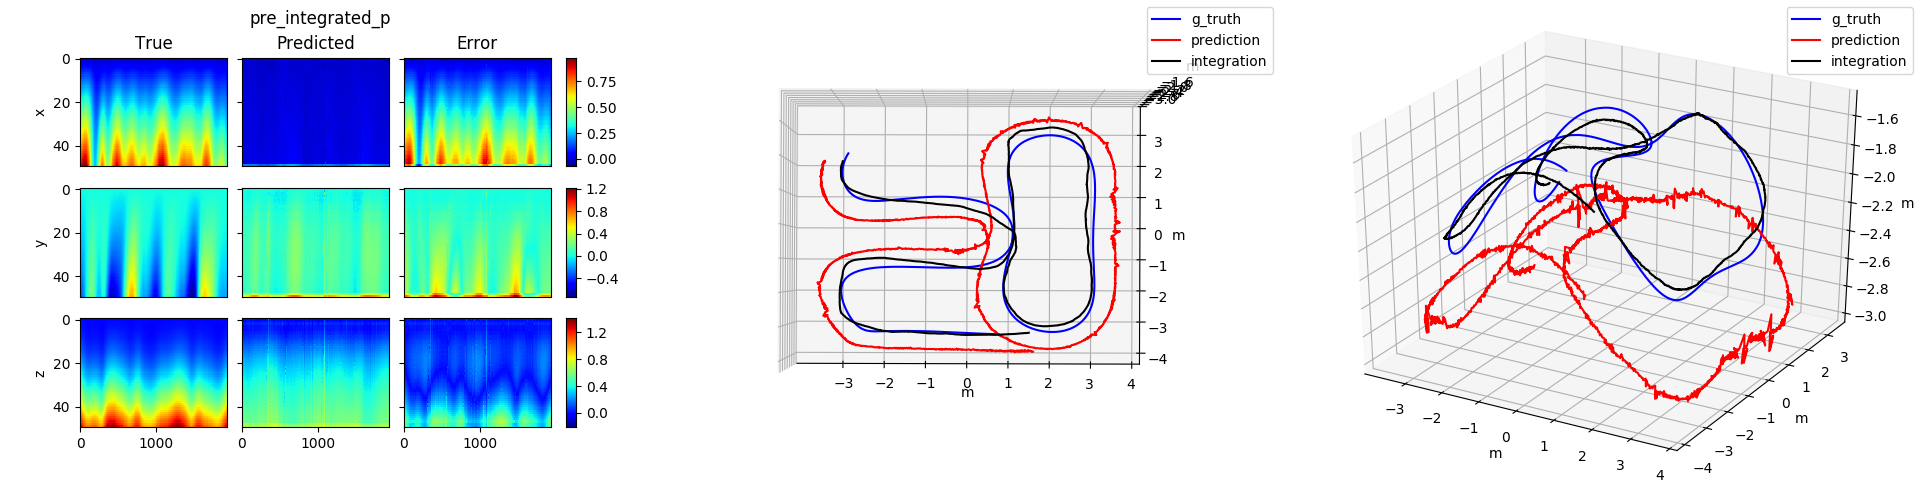
\includegraphics[width=0.95\textwidth]{thesis_template/img/pre_integrated_p_overtuned_results.jpg}
   \caption{Pre-integrated and output position vectors of the one-step experiment on the \emph{bentDice}@2m/s validation set. The \emph{diffusion} regularization term has been over-tuned and the training procedure prioritizes the optimization of this loss factor rather than the actual task loss. 
   This translates into an under-estimated position pre-integration output. 
   However, the results are much more consistent between them than in Figure \ref{fig:position_3D_original_4loss_bentDice_vs_tiltedThrice}.}
   \label{fig:position_overtuned_reg_bentDice}
\end{figure}

After several iterations of trial-and-error, the best parameter combination we find for the loss hyperparameters are: $r_\nabla=0.005$ and $b=0.5$.
With this setup, the we get the results provided in Figure \ref{fig:pre_integration_p3d_best}, on the validation sets \emph{bentDice}@2m/s and \emph{tiltedThrice}@6m/s.
Although we can see in the error plots that the model reasonably outperforms double integration, it is failing to estimate especially the z component of position. 

\begin{figure}[h]
   \centering
   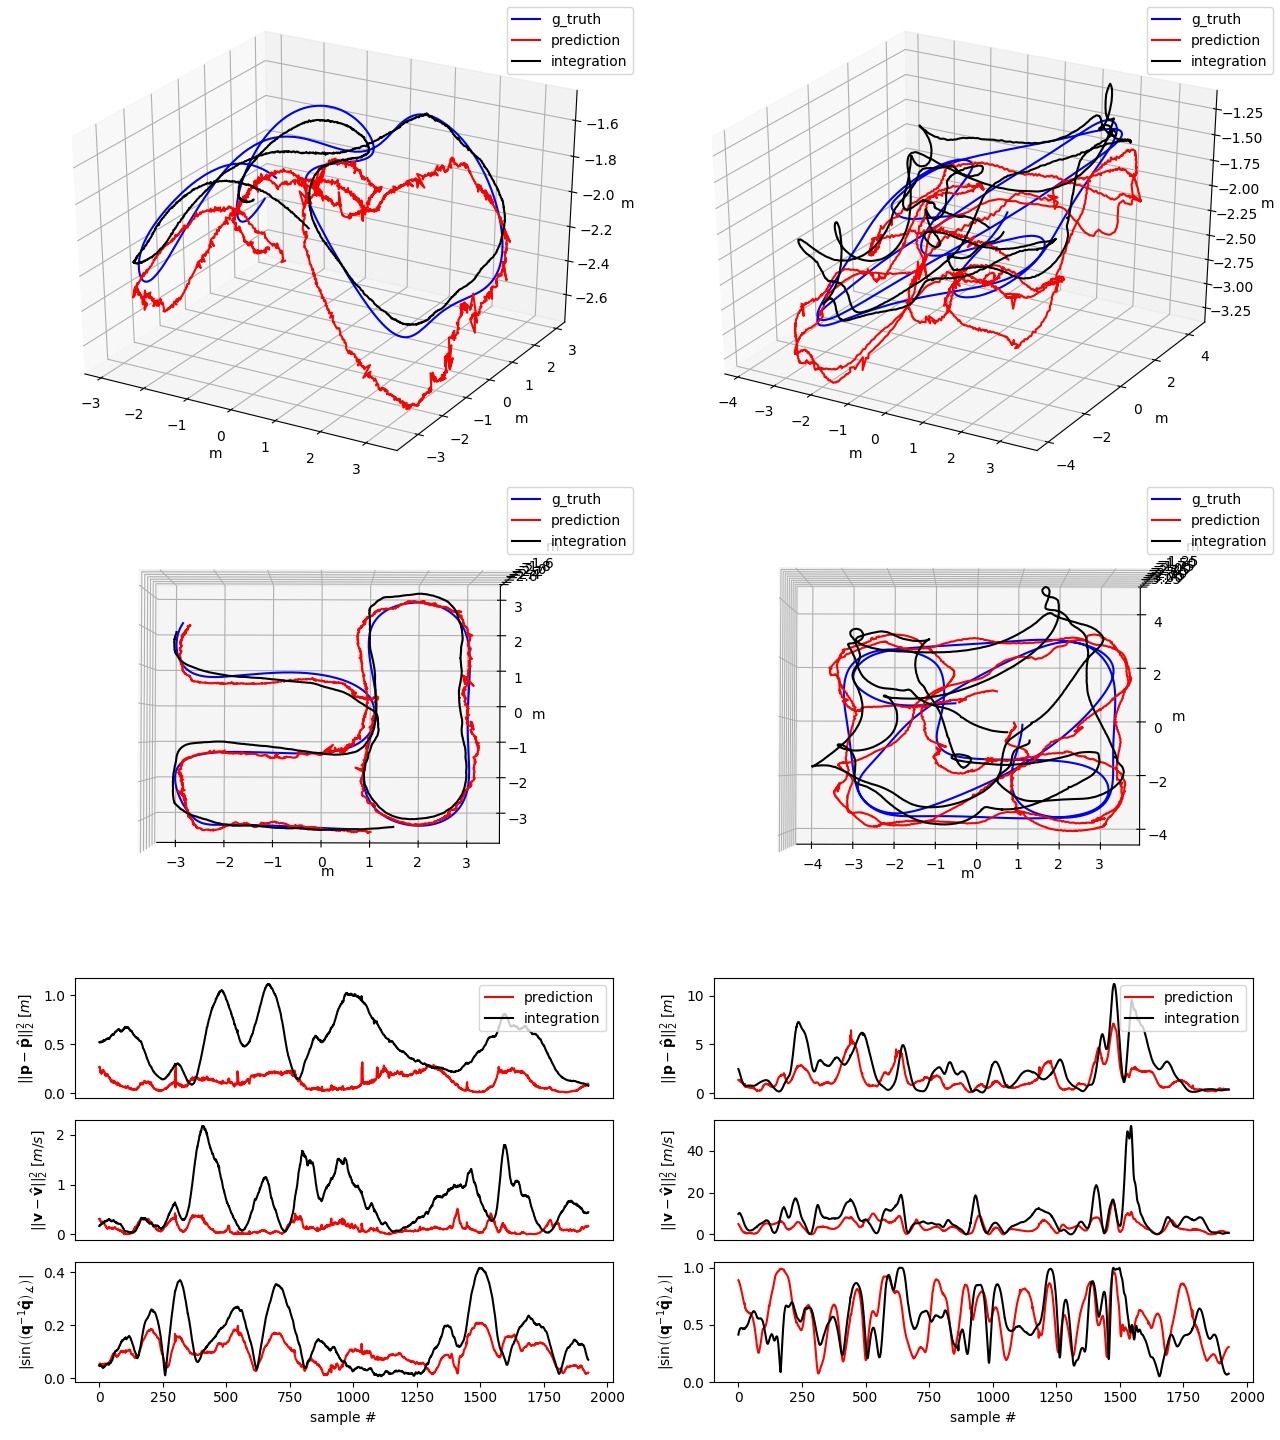
\includegraphics[width=0.95\textwidth]{thesis_template/img/pre_integration_p3d_best.jpg}
   \caption{Position vector output of the one-step experiment on the validation sets \emph{bentDice}@2m/s (1st. column) and \emph{tiltedThrice}@6m/s (2nd column).}
   \label{fig:pre_integration_p3d_best}
\end{figure}

If we perform instead the \emph{iterative} experiment with this last version of the trained model, we verify that this model is not able to compensate the drift (see Figure \ref{fig:pre_integration_iterative_validation}), although it manages to reduce it when compared to IMU integration, both in the position and velocity estimates.
It is difficult to assess whether the rotation estimate is better or worse in the predicted case compared to the integrated one.

\begin{figure}[h]
   \centering
   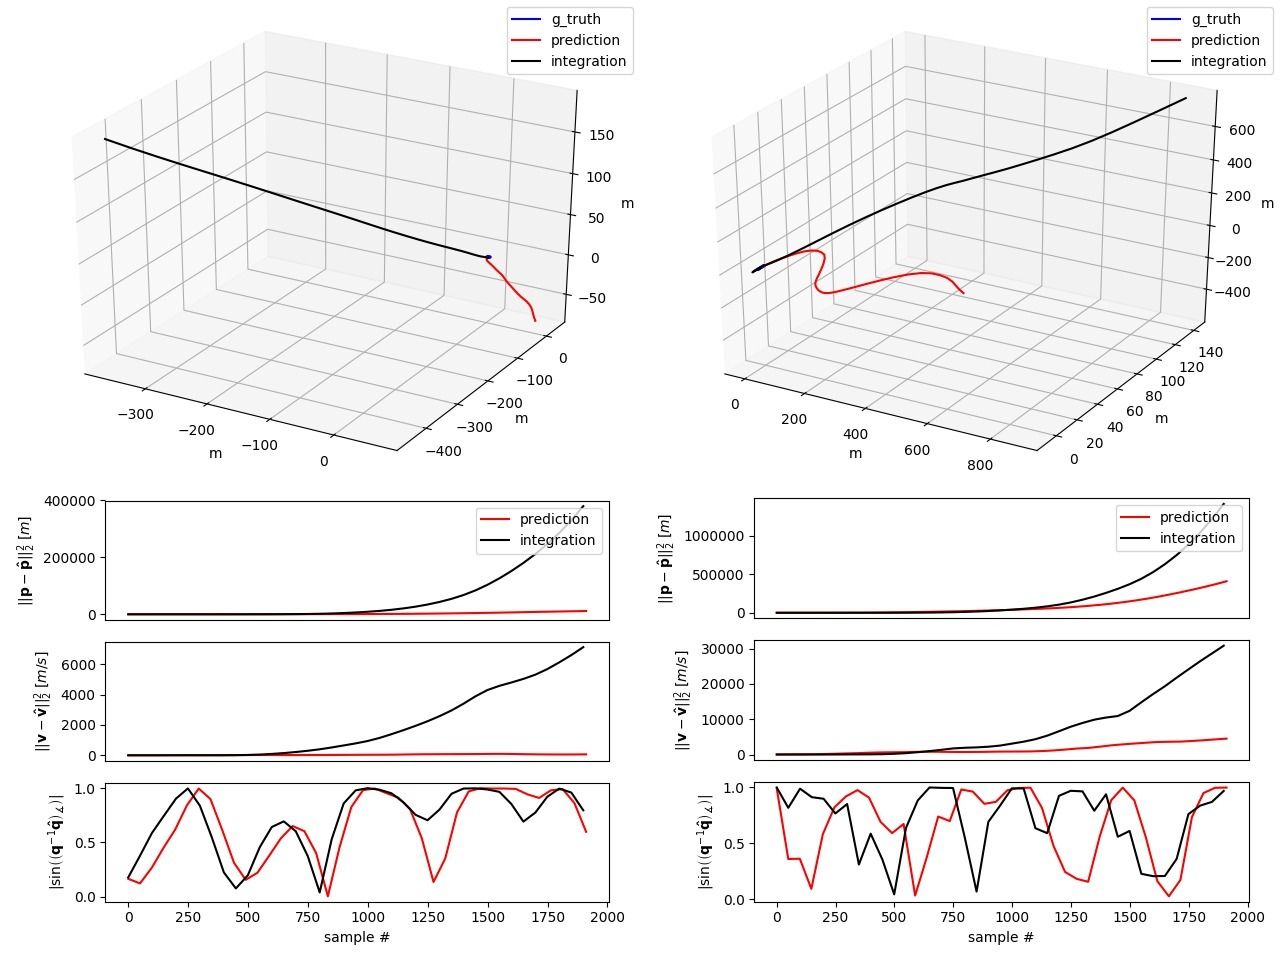
\includegraphics[width=0.95\textwidth]{thesis_template/img/iterative_experiment_pre_integration_pos.jpg}
   \caption{Position vector output of the iterative experiment on the validation sets \emph{bentDice}@2m/s (1st. column) and \emph{tiltedThrice}@6m/s (2nd column).}
   \label{fig:pre_integration_iterative_validation}
\end{figure}

\section{General comparison}

As a wrap-up of the results so far, we run both the one-step and iterative tests for the three available versions of IMU integration deep models.
These three are the two versions of the normal integrator model from Section \ref{sec:imu_state_int} (with quaternion and $\mathfrak{so}(3)$ rotation representation) and the proposed pre-integration model from Section \ref{sec:pre_int_training}.
Also, for each experiment, three datasets are used.
The first is the training dataset, which is a long sequence used for training the models (the first 90\% of the \emph{bentDice}@2m/s dataset). 
The second is the remaining kept-aside 10\% of the training dataset, labeled as test easy (E).
Finally the last is a short sequence of the same length as test (E) from the much harder (H) set \emph{tiltedThrice}@6m/s.
The error terms of the three model predictions are computed from the ground truth data by computing the squared l2 norm, and the average value over the entire used sequence is obtained. 
The results of these experiments are summarized in Table \ref{table:model_comparisons}.

\begin{table}[]
\begin{tabular}{c|c|ccc|ccc|}
\cline{3-8}
\multicolumn{2}{c|}{\multirow{3}{*}{}}                           & \multicolumn{6}{c|}{\textbf{experiment}}                                                                                                                                          \\ \cline{3-8} 
\multicolumn{2}{c|}{}                                            & \multicolumn{3}{c|}{one-step}                                               & \multicolumn{3}{c|}{iterative}                                                             \\ \cline{3-8} 
\multicolumn{2}{c|}{}                                            & \multicolumn{1}{c|}{train} & \multicolumn{1}{c|}{test (E)} & test (H)       & \multicolumn{1}{c|}{train} & \multicolumn{1}{c|}{test (E)} & \multicolumn{1}{c|}{test (H)} \\ \hline
\multicolumn{1}{|c|}{\multirow{4}{*}{\rotatebox[origin=c]{90}{$\left\|\mathbf{p}^e\right\|_2^2$\;[m]}}}   & int     & 0.675                      & 0.644                         & 1.067          & 6.035                     & 5.550                        & 5.809                        \\
\multicolumn{1}{|c|}{}                                & $\mathfrak{so}(3)$     & \textbf{0.179}             & \textbf{0.182}                & \textbf{0.669} & \textbf{4.431}            & \textbf{4.215}               & \textbf{4.502}               \\
\multicolumn{1}{|c|}{}                                & pre-int     & 0.359                      & 0.344                         & 1.234          & 5.7e3                      & 50.990                         & 2.9e2                         \\
\multicolumn{1}{|c|}{}                                & IMU 2int & 0.713                      & 0.731                         & 1.583          & 1.8e4                      & 2.5e2                         & 4.7e2                         \\ \hline
\multicolumn{1}{|c|}{\multirow{4}{*}{\rotatebox[origin=c]{90}{$\left\|\mathbf{v}^e\right\|_2^2\;\left[\frac{m}{s}\right]$}}} & int     & 0.100                      & 0.122                         & 0.217          & 0.249                      & 0.257                         & \textbf{0.350}                \\
\multicolumn{1}{|c|}{}                                & $\mathfrak{so}(3)$     & \textbf{0.071}             & \textbf{0.077}                & \textbf{0.182} & \textbf{0.184}             & \textbf{0.219}                & 0.424                         \\
\multicolumn{1}{|c|}{}                                & pre-int     & 0.370                      & 0.356                         & 1.933          & 2.8e2                      & 6.170                        & 38.730                         \\
\multicolumn{1}{|c|}{}                                & IMU 2int & 0.826                      & 0.810                         & 2.727          & 2.9e2                      & 43.589                         & 84.853                         \\ \hline
\multicolumn{1}{|c|}{\multirow{4}{*}{\rotatebox[origin=c]{90}{$\sin\mathbf{q}^e_\measuredangle$[rad]}}}       & int     & 0.482                      & 0.433                         & 0.619          & \textbf{0.540}             & \textbf{0.282}                & \textbf{0.129}                \\
\multicolumn{1}{|c|}{}                                & $\mathfrak{so}(3)$     & 0.252                      & 0.274                         & 0.612          & 0.574                      & 0.591                         & 0.676                         \\
\multicolumn{1}{|c|}{}                                & pre-int     & \textbf{0.086}            & \textbf{0.097}                & 0.563          & 0.642                      & 0.655                         & 0.657                         \\
\multicolumn{1}{|c|}{}                                & IMU 2int & 0.121                      & 0.148                         & \textbf{0.533} & 0.644                      & 0.710                         & 0.708                         \\ \hline
\end{tabular}
\captionof{table}{Performance comparison of the three IMU integration models with vanilla double integration.
The errors are computed with the loss functions described by \ref{eq:q_state_loss} with the ground truth data.
The models are tested on the long training set, an two shorter test sets, labeled as easy (E) and hard (H).
The easy test set is a held-out test set from \emph{bentDice}@2m/s and the hard set is a fragment of \emph{tiltedThrice}@6m/s, of the same length as the easy test set.
Results show that $\mathfrak{so}(3)$-based integration model outperforms the rest on nearly all experiments for both position and velocity estimation. 
The best rotation results are much more inhomogeneous.
    \label{table:model_comparisons}}
\end{table}

An analysis of such table shows that the $\mathfrak{so}(3)$-based state integrating model outperforms the rest in almost all cases for the position and velocity estimates.
More particularly, it achieves an error for position in the difficult test set in the one-step integration experiment of $\sqrt{0.448}=0.67m$, which is significantly lower than in the other cases.
It also behaves much better than the other models in the iterative experiment, because as we saw in Figures \ref{fig:imu_so3_bentdice_val} and \ref{fig:imu_so3_tiltedThrice_val}, the estimate does not drift away from the span of the input data.
This, however, does not really mean that its predictions are good for this case, as it can also be seen in the same two figures.
Unfortunately, the metrics for the rotation prediction are not very reliable for determining which model performs better or worse at this case, as the error cannot be defined in an euclidean way.
In fact, no matter if we use Lie Algebra or quaternions as rotation base, the rotation error is periodic, and therefore especially in the iterative case, the metrics are not very useful to actually infer the performance of the model.
However, for the one-step experiment, where rotations are small enough for not going through sign flips in one window, it looks like indeed the $\mathfrak{so}(3)$ formulations of the second and third models help to learn better the rotation term.


\chapter{Discussion}\label{chap:discussion}

\section{Conclusion}\label{sec:conclusion}

In this work, we have reviewed the current state-of-the-art of deep learning-based inertial odometry.
We have reproduced and adapted some of the results available, which in all cases are framed in 2D environment such as in autonomous car driving or walking, into the more challenging 3D setup of agile aerial units. 
We decide to constrain our research to two well-known, publicly available MAV datasets: the EuRoC and the BlackBird.
Although our results are based on a selection of the flights available in both datasets, our approaches are generalizable to any similar data framework.
Despite that, we also remark the fact that every dataset has a unique IMU sensor with unique intrinsic parameters, so most likely our models would need to be re-trained for every dataset.
In other words, it is very possible that any deep learning model for inertial odometry has to be trained with the specific IMU that is going to be used at inference time. 

In particular, we have tackled two different estimation tasks using IMU data as the prediction foundation, from three different perspectives, where each one builds up on the knowledge gathered by all the previous experiments.
We believe our research pushes the understanding of the problem of DL-based IO towards a more reliable solution, and we propose several ways of continuing our research that we believe are promising.

In particular, we have started our research by re-implemented a convolutional deep model from the literature to regress the speed magnitude of a drone just from IMU measurements.
We argue why this problem setup is ill-posed, since the speed cannot be properly predicted from inertial data without an initial value, and remark the positive and negative characteristics of the proposed architecture for this task.
We show that this trained model, that can perfectly fit a training dataset, is not properly predicting on any other test set not used in training time.
However, we also validate the model performance with an ideal IMU measurement dataset without noise, and obtain interesting results which suggest that actually the speed estimate might have some meaning after all.

Next, we reformulate the problem into replicating the IMU integration process with a deep model.
Given an initial 10-dimensional state, and a window of IMU data, we predict the state at the end of such window.
Our hope is that the deep model can learn to overcome the inherent noise of this kind of inertial sensor, which renders vanilla IMU integration not reliable for inertial odometry on its own.
We propose a simpler CNN model inspired by the best features of the previous one, that helps to debug better which architectures work and which don't for this task.
We show that convolutional layers are likely to be a good idea for processing IMU data, but we also reason why using the initial state as an input increases the risk of over-fitting during training time. 
We also expand an idea from the literature to help a model learn from rotations in quaternion form, by using their Lie Algebra representation.
We show that this change helps significantly in integrating the rotation state, and subsequentially improves the quality of the overall prediction.
With this approach, we obtain a model that outperforms IMU integration, but is still unreliable as a long-term odometer.

For our final study, we continue working on the same IMU integration task, but we incorporate yet another concept from the literature.
The latter allows to compute a \emph{state increment} just from IMU data, without relying on any input state whatsoever, whose mathematical reasoning is based on the \emph{pre-integration} theory.
We propose a very lightly parametrized deep model which combines multiple architectural ideas from the literature, with a customized operational flow to reinforce some theoretically founded inter-dependencies between intermediate output variables.
We train this model to learn to estimate the pre-integrated states, and apply them in a non-trainable manner to an input state to generate an output state prediction.
Although this approach looks promising, its proves to be equally challenging to properly train.
We propose several improvements that help fine-tune the model, although unfortunately we don't manage to fully recover the optimal parameter set.

As a wrap up, we compare the last three models for IMU state integration on three different datasets to evaluate their performance against each other and vanilla IMU double integration.
We show that so far the best model obtained for short and long term state integration is the Lie Algebra-based model.
Namely, this model, although it is not able to properly follow a state sequence just from an initial state and a chain of IMU data, manages not to drift away from the span of the data.
On the other hand, all three models almost consistently outperform double-integration for all the components of the state, with the exception of the rotation term.

Despite this quantitative result, we believe that the formulation of the pre-integration model is very promising.
Its current problem is that, due to the fact that the four output values are dependent on each other, an error on the one of them immediately translates to errors in the rest.
This problem makes the training of this architecture very challenging, as all variables must be optimized at once.
For this reason, we believe that this model requires a probabilistic reformulation so that it can handle uncertainty.
Furthermore, if it could also retain information from previous predictions to predict the next iteration, then the outputs could gain a lot in temporal consistency.
A first approach for the memory idea be actually quite easy to implement, as the current recurrent generative layers could accept as input the hidden states from the previous iteration of predictions.
Right now, for every prediction these hidden states are initialized from 0, and thus the model does not keep information between different windows.


\section{Future Work}\label{sec:future_work}

We believe our three studied models, and especially the last one, have plenty of room for interesting improvements that could help in the problem of IO.

Although we know that the speed regressor is most likely unreliable for predicting the speed state, we have seen that it might actually be useful as a low-confidence measurement update in a nonlinear estimation pipeline.
Maybe a similar approach, with a much lighter model, could be used as a measurement system in, for example, an Extended Kalman Filter.

So far, our second model has probably shown the best results in terms of long-term state prediction. 
Furthermore, despite our reasoning that its setup might be prone to over-fitting the data, we also show that it is not the case for our model.
Finally, we also provide empirical data that indicates that some of its architectural features are introducing more noise than helping, so removing these and training again the model in similar conditions could be an approach worth trying.

And regarding our third model, we are convinced that its theoretical background is powerful enough for it to eventually become a good estimator.
According to our opinion, there are two very interesting improvements that could be performed on it.
\begin{itemize}
    \item Instead of trying to predict a final state from the initial state, predict a probability distribution of final states, given a probability distribution of initial states. 
    This would allow the model to perform some kind of estimate update, given the likelihood of input states.
    \item Related with the previous point, the pre-integrated state generators in our model are three recurent GRU cells. 
    It would be very interesting if these cells could recover the hidden state from the last prediction, and use it as initial hidden state.
    Perhaps the model then could be trained to pass on some information for the next prediction iteration that could help it gain some temporal consistency in between windows of time.
\end{itemize}

\cleardoublepage

% Appendix______________________________________________________________________
\appendix
\chapter{Appendix}\label{chap:appendix}

\subsection{Learning from the inertial EuRoC dataset}\label{sec:euroc_filtering}

The EuRoC dataset \cite{Burri25012016} contains IMU measurements at 200Hz and 6-DoF ground-truth estimates captured using a Vicon motion capture system at 100 Hz. 
After some testing in section \ref{sec:speed_reg}, we empirically show that a heavily parametrized deep model can be successful at fitting the training datasets for partial state prediction from just the IMU data, whether that is an overfit or not.
To be able to do it, however, a low-pass pre-processing of the EuRoC dataset is employed, as the IMU data and especially the accelerometer data are quite noisy for this dataset.
This low pass filtering is found to be \textbf{critical} when fitting in the model, as without it even a model with 18 million parameters is not able to overfit a 1-dimensional output.

The EuRoC flights used (Machine Hall 1 \& 2) can be divided in two sequences separated by a still period.
During the first 20 seconds approximately, the drone is picked up and moved by hand; then it is left back on the floor for a few more seconds, and finally (starting around second 30) it is remotely piloted for a longer period of time.
This fact helps us realize that the increased noise in the accelerometer is present only during the second sequence, when the drone is flying, as it can be seen in Figure \ref{fig:filtEuroc} (top).
We thus hypothesize that the increased noise is probably produced by the vibration of the rotors, and proceed to study if it can be safely removed with some filtering technique.

\subsubsection{Low pass filtering of MAV's inertial data}

After inspection of the Short Time Fourier Transforms (STFT) of the IMU and the ground truth data, we confirm that there is a very significant increase of high frequency components during the second sequence, which are completely not present in the first sequence (especially around the frequency range of 20-30 Hz for the $y$ component).
This leads to the hypothesis that rotor noise can be safely removed with a low-pass filter without affecting to the overall IMU data quality.
The filter employed is chosen to be the Butterworth filter, which has two design parameters: the degree of the filter $n$ and the cutoff frequency $f_0$. 
The reason behind the usage of the Butterworth filter, is that it keeps the frequencies in the pass band almost unaltered, which in our case we assume contain the most relevant information about the trajectory of the flying unit.
We chose $f_0$ to be 10Hz, as in the STFT diagram the components above this frequency in the first part (manual motion) are significantly reduced.
We then select $n$ by trial and error, picking up the smallest value that still \emph{attenuates enough}, the high frequency noise, so that the noisy region resembles the manual motion. 
We find $n=3$ to be a good value for this parameter, which led to the results shown in Figure \ref{fig:accSTFT}.
\begin{figure}
    \centering
    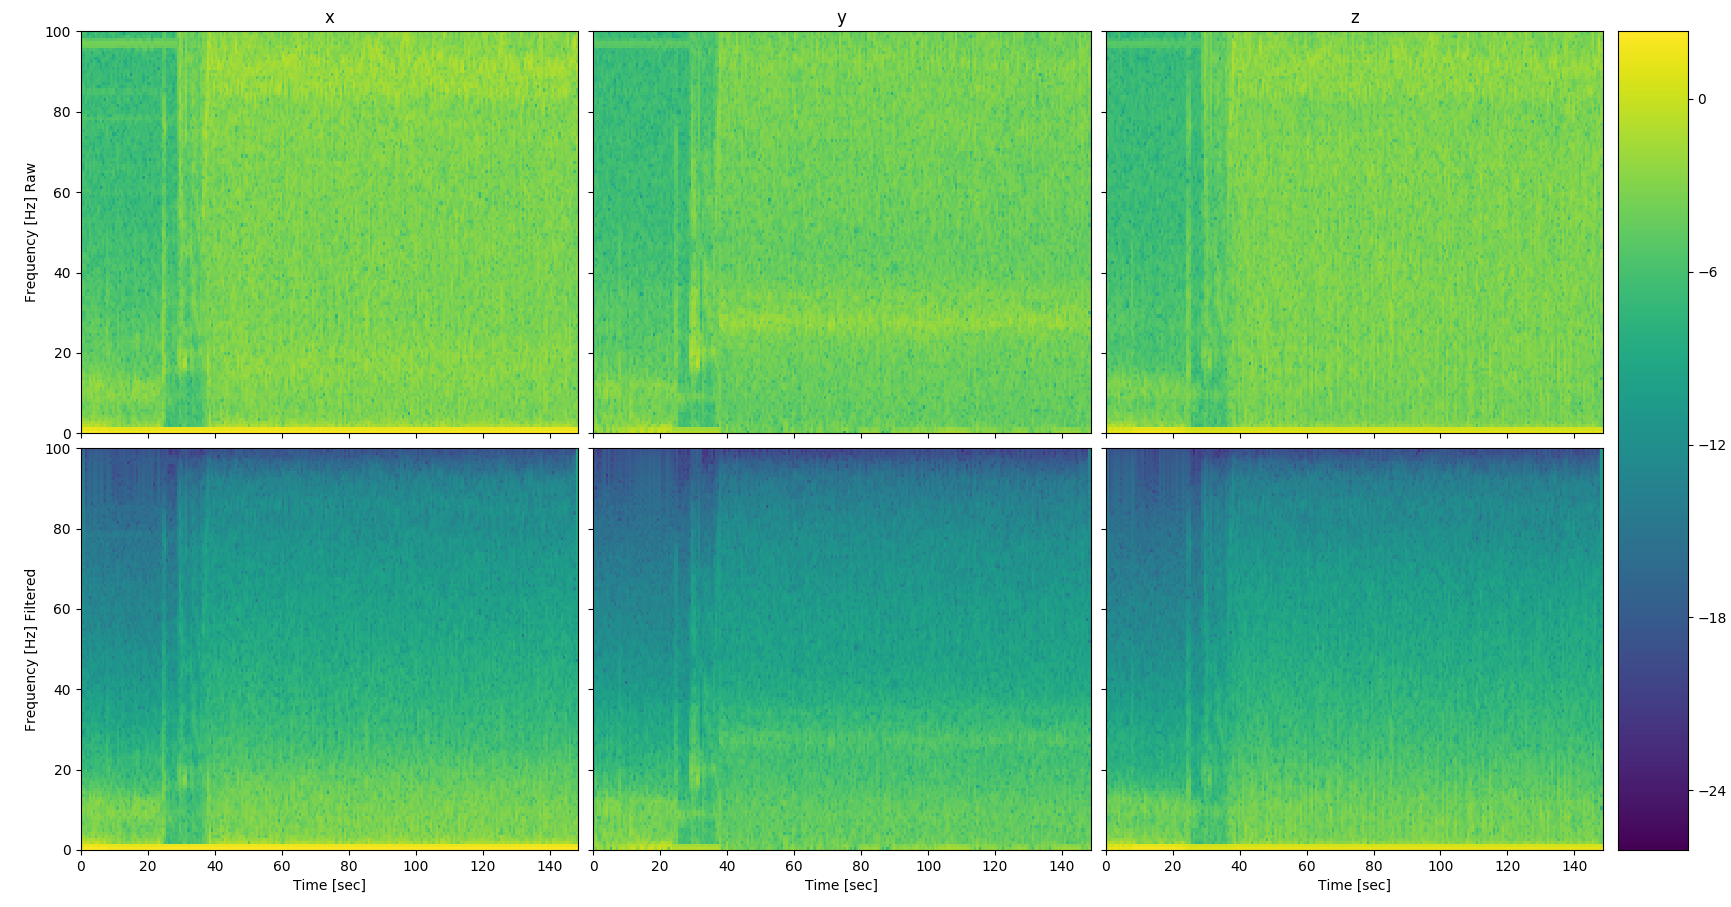
\includegraphics[width=\textwidth,height=\textheight,keepaspectratio]{thesis_template/img/accSTFT.png} 
    \caption{STFT of the accelerometer readings before (top row) and after (bottom row) the application of a low-pass filter (log scale)}
    \label{fig:accSTFT}
\end{figure}
It can also be appreciated in the time domain signal (Figure \ref{fig:filtEuroc} (bottom) that a large portion of the noise has indeed disappeared.
This, more importantly, leads to the model being able to fit with much more precision the training data.
One may also notice in Figure \ref{fig:filtEuroc}, that the \emph{flat} region of the dataset has been expanded. 
We do this because we empirically find that it helped to determine the \emph{resting state} for the model, i.e. when the drone is not moving at all. 
\begin{figure}
    \centering
    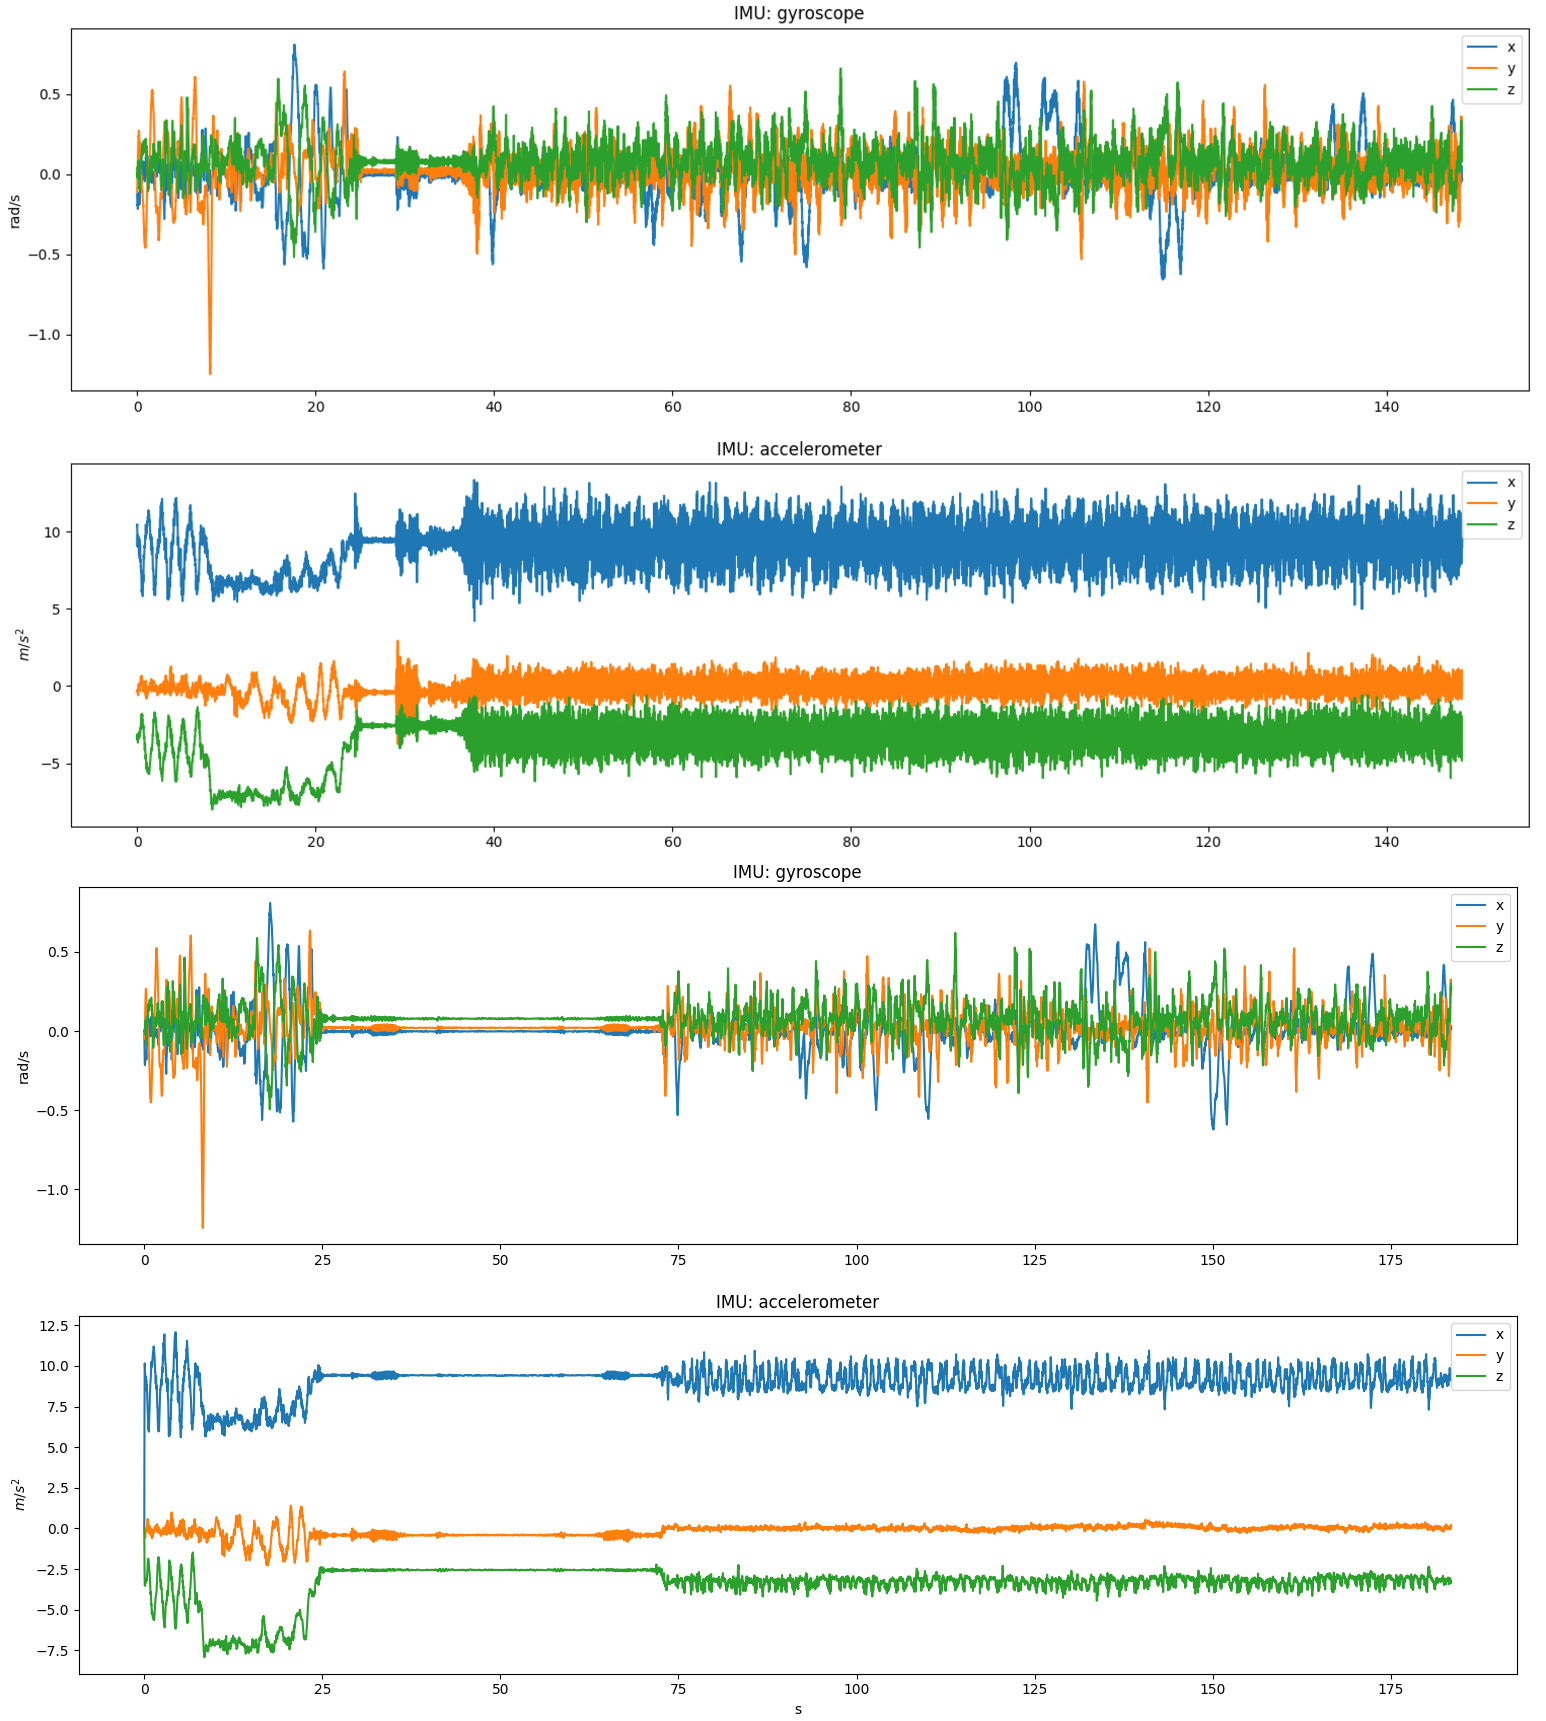
\includegraphics[width=\textwidth,height=\textheight,keepaspectratio]{thesis_template/img/euroc_imu_filtering.jpg} 
    \caption{Unfiltered (top two) and filtered (bottom two) IMU readings of flight "Machine Hall 2" from the Euroc dataset}
    \label{fig:filtEuroc}
\end{figure}

As a last verification step, in Section \ref{sec:speed_regression_model}, we evaluate the performance of the model with the ideal version of the EuRoC dataset with and without noise, and check that its predictions are nearly identical.

For this reason, from we always perform this low-pass filtering for all our inertial data, as it was found to help a lot during training.

\cleardoublepage

% Bibliography__________________________________________________________________

\bibliographystyle{IEEEtran}
\bibliography{bibtex/references.bib}
\bibliographystyle{unsrt}
\end{document}
